%\documentclass[11pt,a4paper,english,twoside]
\usepackage{epsfig}\usepackage[explicit]{titlesec}
%\usepackage{indentfirst}
%\usepackage{verbatim}
%\usepackage{amsmath}
%\usepackage{subcaption}
%\usepackage{amsthm}
%\usepackage{amssymb}
%\usepackage{epstopdf}
%\usepackage{latexsym}
%\usepackage{index}
%\usepackage{datetime}
%\usepackage{textcomp}
%\usepackage{graphicx}
%\usepackage{url}
%\usepackage{array}
%\usepackage{algorithm}
%\usepackage{algorithmic}
%\usepackage{babel}
%\usepackage{afterpage}
%\usepackage{caption}
%\usepackage{makeidx}
%\bibliographystyle{alpha}
%\bibliographystyle{abbrv}

%\newindex{default}{idx}{ind}{Ευρετήριο όρων}
%\newindex{en}{edx}{end}{Ευρετήριο αγγλικών όρων}
%\makeindex


% Page definitions
%\setlength{\textheight}{23cm} \setlength{\textwidth}{15.5cm}
%\setlength{\oddsidemargin}{0.2cm}
%\setlength{\evensidemargin}{0.2cm} \setlength{\topmargin}{-1.2cm}
%\setlength{\headsep}{1.5cm}

% 1.5 spacing
%\renewcommand{\baselinestretch}{1.2}

%\newcommand\blankpage{%
%    \null
%    \thispagestyle{empty}%
%    \addtocounter{page}{-1}%
%    \newpage}
% latin text (and greek text)
%\newcommand{\prg}[1]{\textlatin{\texttt{#1}}}
%\newcommand{\tl}[1]{\textlatin{#1}}
%\newcommand{\tg}[1]{\textgreek{#1}}

% typeset short english phrases
%\newcommand{\en}[1]{\foreignlanguage{english}{#1}}

% typeset source code
%\newcommand{\src}[1]{{\tt\en{#1}}}



% typeset a backslash
%\newcommand{\bkslash}{\en{\symbol{92}}}

%typeset infx(a) supx(a) etc
%\newcommand{\infx}[1]{inf_x({#1})}
%\newcommand{\infy}[1]{inf_y({#1})}
%\newcommand{\supx}[1]{sup_x({#1})}
%\newcommand{\supy}[1]{sup_y({#1})}
%\newcommand{\dlt}{\delta}
%\newcommand{\most}{${\cal M}ost$}
%\newcommand{\br}{${\cal B}r$}
%\newcommand*\Hide{%
%\titleformat{\chapter}[display]
%  {}{}{0pt}{\Huge}
%\titleformat{\part}
%  {}{}{0pt}{}
%}
%\newtheorem{definition}{Ορισμός}
%\newtheorem{proposition}{Πρόταση}
%\newtheorem{theorem}{Θεώρημα}
%\newtheorem{corollary}{Συμπέρασμα}
%\newtheorem{lemma}{Λήμμα}
%\newtheorem{example}{Παράδειγμα}
%\newtheorem{remark}{Σημείωση}
%\newtheorem{notation}{Συμβολισμός}
%\newtheorem{law}{Νόμος}
%\renewcommand{\thedefinition}{\arabic{chapter}.\arabic{definition}}
%\renewcommand{\theproposition}{\arabic{chapter}.\arabic{proposition}}
%\renewcommand{\thetheorem}{\arabic{chapter}.\arabic{theorem}}
%\renewcommand{\thecorollary}{\arabic{chapter}.\arabic{corollary}}
%\renewcommand{\thelemma}{\arabic{chapter}.\arabic{lemma}}
%\renewcommand{\theexample}{\arabic{chapter}.\arabic{example}}
%\newcommand{\set}[1]{\left\{#1\right\}}
%\newcommand{\To}{\Longrightarrow}
%\newcommand{\xml}{\en{XML}}


%\selectlanguage{greek}
%\hyphenation{τμή-μα Επο-μέ-νως}

%\title{Σύγκριση και ανάπτυξη ασαφών μέτρων ομοιότητας και συσχέτισης δεδομένων αισθητήρων σε εφαρμογές υγείας και περιβάλλοντα υποβοηθούμενης διαβίωσης.}
%\author{Νίκος Τερλεμές}
%\supervisor{Δημήτριος Κουτσούρης}
%\TRnumber{ΕΒΤ-ΔΙΠΛ-2017-10}
%\epitropiF{?}
%\epitropiS{?}


 	 	
\begin{document}
%\selectlanguage{greek}
%\maketitle

%\frontmatter
%\pagenumbering{roman}
%\mainmatter
%\begin{acknowledgements}
Θα ήθελα να ευχαριστήσω τον τάδε.
\end{acknowledgements}


\begin{abstract}
Οι ολοένα και αυξανόμενες δυνατότητες της επίστημης υλικών και της ηλεκτρονικής έχουν επιτρέψει την ανάπτυξη και την μαζική παραγωγή κάθε είδους αισθητήρων.
Αυτή η εξέλιξη, δημιούργησε την ανάγκη της διαχείρισης αυτών και της πληροφορίας που παράγουν, καθώς και νέες δυνατότητες αξιοποιήσης τους.
Αυτές τις ανάγκες και προβλήματα λύνει ο τεχνολογικός κλάδος, ο οποίος ονομάζεται διαδίκτυο των πράγματών (\en{Internet of Things}).
Ένας από τους κλάδους που επηρεάστηκαν από την δυνατότητα δημιουργίας και διαχείρησης περιβάλλοντων διάχυτης τηλεπισκόπησης, είναι η Βιοϊατρική, καθώς πλέον είναι εφικτή η απρόσκοπτη ανάλυση δεδομένων από αισθητήρες κάθε είδους.
Ωστόσο, παραμένει μεγάλη πρόκληση για τον τομέα η ανάλυση δεδομένων από μεγάλο πλήθος αισθητήρων, όπως σε ένα Περιβάλλον Υποβοηθούμενης Διαβίωσης (ΠΥΔ).
Oι εξελίξεις σε άλλα ερευνητικά πεδία, όπως ο τομέας της Μηχανικής Μάθησης, έχουν οδηγήσει στην επίλυση παρόμοιων προβλήματων, οπότε είναι συχνή η χρήση τέτοιων τεχνικών στην ανάλυση δεδομένων από ΠΥΔ.
\par
Με βάση τα παραπάνω, η παρούσα διπλωματική εργασία σκοπεύει στη μελέτη, σχεδίαση και ανάπτυξη αλγορίθμων αναζήτησης, σύγκρισης και συσχέτισης δεδομένων αισθητήρων, ανεξάρτητα από το πλαίσιο τους, προκειμένου να επιτρέψει την καλύτερη διαχείριση δεδομένων από ΠΥΔ.
Συγκεκριμένα, συγκρίνει και αναπτύσσει μετρικά ομοιότητας δεδομένων αισθητήρων, δίνοντας ιδιαίτερο βάρος σε μετρικά τα οποία προκύπτουν από την θεωρία ασαφών συνόλων.
\par
Η παρούσα εργασία αποτελείται από 5 ενότητες.
Στην πρώτη ενότητα, παρουσίαζονται οι ιδέες και έννοιες που απαρτίζουν τον τομέα του \en{Internet of Things}, της Βιοϊατρικής, της Μηχανικής Μάθησης καθώς και της τομής τους.
Στη δεύτερη ενότητα, παρουσιάζεται ο κλάδος των ΠΥΔ, οι σύγχρονες προσεγγίσεις και τεχνολογίες που τον απαρτίζουν και περιγράφεται το πρόβλημα της αναζήτησης και σύγκρισης μεγάλου όγκου δεδομένων από μεγάλο πλήθος αισθητήρων, το οποίο αποτελεί το θέμα αυτής της εργασίας.
Στην τρίτη ενότητα μελετάται ο τομέας της Θεωρίας Ασαφών Συνόλων και αναδεικνύεται σαν πιθανή λύση στο πρόβλημα η χρήση μετρικών ομοιότητας, βασισμένα σε ασαφή σύνολα.
Στην τέταρτη ενότητα, παρουσιάζεται το σύνολο δεδομένων \en{Opportunity}, πάνω στο οποίο στηρίχτηκε αυτή η εργασία., το οποίο περιέχει δεδομένα από σενάρια καθημερινών δραστηριοτήτων σε ΠΥΔ, εξοπλισμένο με 44 ετερογενείς αισθητήρες.
Επίσης, παρουσιάζονται αναλυτικά οι τεχνικές για την κατασκευή ασαφών συνόλων από δεδομένα αισθητήρων και τα μετρικά ομοιότητας αισθητήρων τα οποία χρησιμοποιήθηκαν για την εργασία αυτή.
Τέλος, στην πέμπτη ενότητα γίνεται η αξιολόγηση και η σύγκριση των παραπάνω τεχνικών, με την χρήση δεδομένων από ΠΥΔ.
\begin{keywords}
Διαδίκτυο των Πραγμάτων, Βιοϊατρική, Περιβάλλοντα Υποβοηθούμενης Διαβίωσης, Μηχανική Μάθηση, Ασαφής Λογική, Αναζήτηση Αισθητήρων, Μετρικά Ομοιότητας, Σύνολο δεδομένων \en{Opportunity}
\end{keywords}
\end{abstract}

%\tableofcontents
%\listoffigures
%\listoftables
%\chapter{Διαδίκτυο των Πραγμάτων και εφαρμογές στην Βιοϊατρική}
\label{chap1}
\section{Διαδίκτυο των Πραγμάτων}
\subsection{Σκοπός}
Κατά την διάρκεια της δεκαετίας 2010-2020, ο όρος Διαδίκτυο των Πραγμάτων (\en{Internet of Things} ή εν συντομία \en{IoT}) αποτέλεσε άλλον έναν αναδυόμενο τεχνολογικό κλάδο, ο οποίος πέρασε από τα διάφορα στάδια αποδοχής και ωρίμανσης του (\en{Hype Cycle}), όπως αποδίδονται γραφικά στο Σχήμα \ref{hc}.
\begin{figure}[h!]
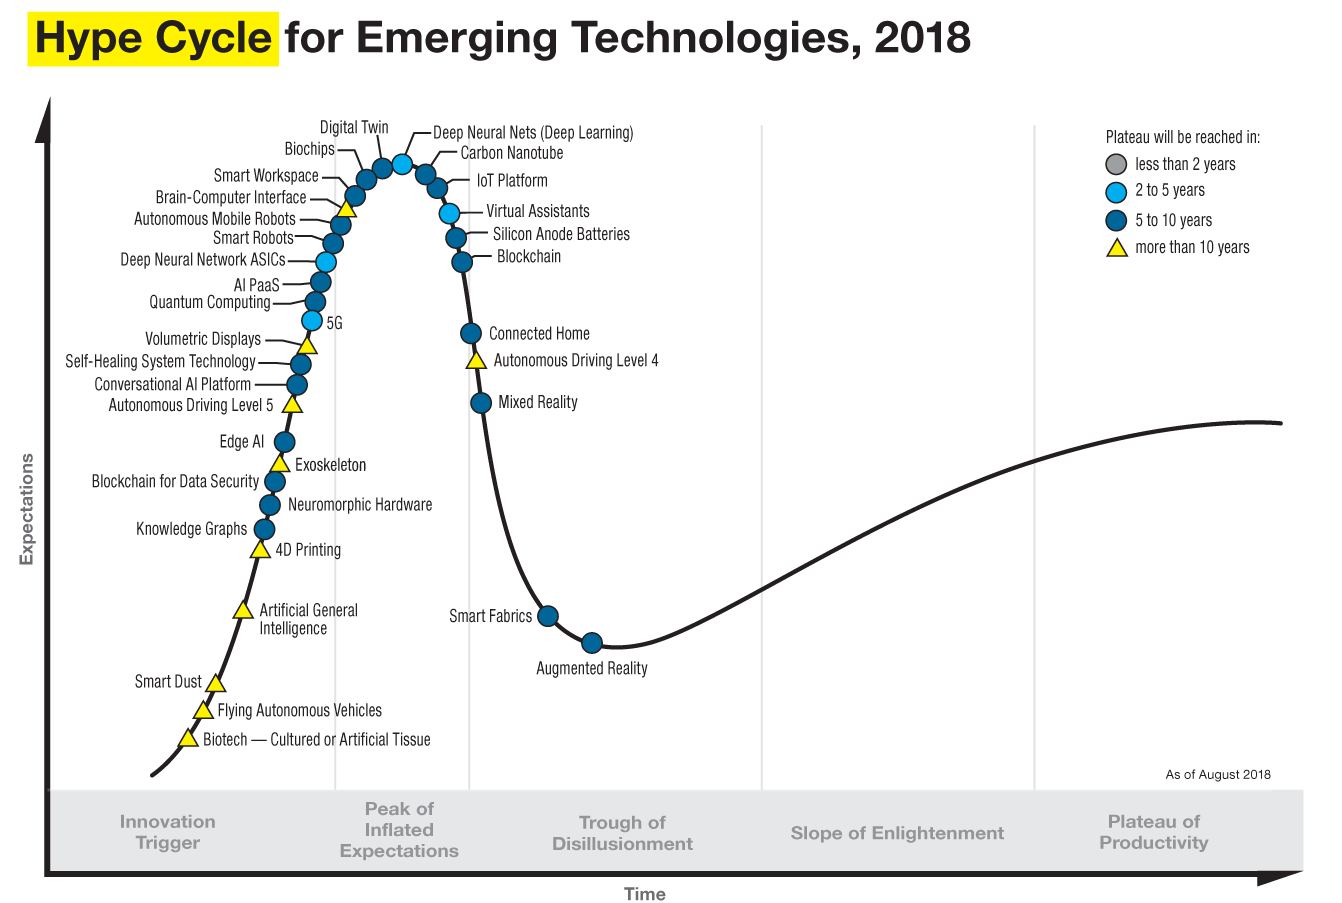
\includegraphics[scale=0.3]{images/hype_cycle.png}
\centering
\caption{Γραφική απεικόνιση της έννοιας του \en{Hype cycle} και απεικόνιση των διάφορων τεχνολογιών το 2018 από την \en{Gartner} \cite{Gartner:HC}}	
\label{hc}
\end{figure}
Λόγω της απόστασης μεταξύ των υψηλών προσδοκιών και των αποτελεσμάτων που έχει αποδώσει ο κλάδος, καθώς και λόγω της ασάφειας που τον περιβάλλει, το Διαδίκτυο των Πραγμάτων αποτελεί πλέον έναν παρεξηγημένο όρο και δεν αναδεικνύεται η ουσία ύπαρξης του.
\par
Το Διαδίκτυο των Πραγμάτων είναι ένας τεχνολογικός κλάδος με αντικείμενο την σχεδίαση και την υλοποίηση της μελλοντικής διεπαφής του φυσικού και του ψηφιακού χώρου.
Ο στόχος είναι ένα περιβάλλον διάχυτης παρουσίας και επισκόπησης, αποτελούμενα από διασυνδεδεμένα αντικείμενα, τα οποία αλληλεπιδρούν με το περιβάλλον τους και συνεργάζονται για την επίτευξη κοινών στόχων. \cite{book:giusto}
\par
Η επίτευξη αυτού του στόχου θα σχηματίσει την καθημερινή ζωή και συμπεριφορά των ανθρώπων της εποχής, όπως, αντίστοιχα, το Διαδίκτυο εξακολουθεί να μετασχηματίζει τις ζωές μας.
Ένα τέτοιο περιβάλλον θα επηρεάσει τομείς όπως η μετακίνηση ανθρώπων και αγαθών, ο αυτοματισμός, η βιομηχανική παραγωγή και τέλος ο τομέας της υγείας.
\par
Προφανώς, οι δυνατότητες αυτές έχουν γίνει αντιληπτές από τον επιχειρηματικό τομέα.
Οι εκτιμήσεις της \en{Cisco} αναφέρουν πως το 2022 θα είναι συνδεδεμένες στο Διαδίκτυο πάνω από 28.5 δισεκατομμύρια συσκευές \cite{cisco2019}, όπως αποδίδεται στο Σχήμα \ref{iotnumb}.
H \en{Gartner, Inc.} εκτιμά πως το 2020 πάνω από τις μισές νέες επιχειρησιακές διαδικασίες και συστήματα θα περιλαμβάνουν κάποιο στοιχείο του \en{IoT} \cite{gartner2016}.
Επίσης, η \en{McKinsey} προβλέπει πως το 2025 η επίδραση του κλάδου στην παγκόσμια οικονομία θα είναι της τάξεως των τρισεκατομμυρίων δολαρίων \cite{mck2016}.

\begin{figure}[h!]
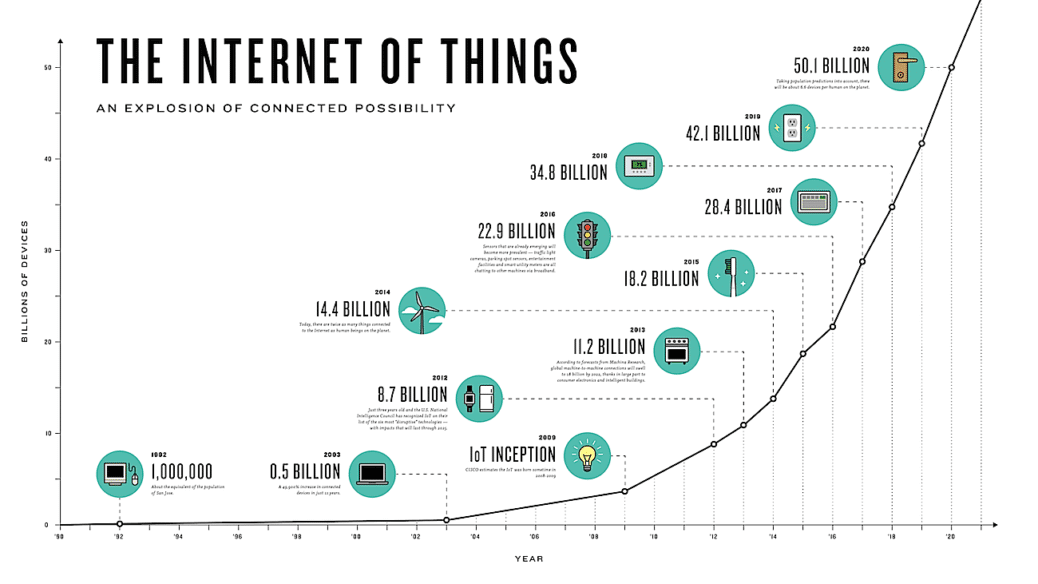
\includegraphics[scale=0.4]{images/IOT_numbes.png}
\centering
\caption{Γραφική απεικόνιση της εξέλιξης του αριθμού των συνδεδεμένων συσκευών στο Διαδίκτυο \cite{iotnumb}}	
\label{iotnumb}
\end{figure}

\subsection{Εισαγωγή}
Το \en{IoT} ορίζεται ως ``ένα παγκόσμιας εμβέλειας δίκτυο από άμεσα προσπελάσιμα, μοναδικά διευθυνσιοδοτημένα, διασυνδεδεμένα αντικείμενα, βασισμένο σε σαφώς ορισμένα πρωτόκολλα επικοινωνίας`` \cite{ATZORI20102787}.
Ουσιαστικά, αποτελεί μια επέκταση του Διαδικτύου, η οποία καθιστά εφικτή την συνδεσιμότητά φυσικών αντικείμενων.
Η επαύξησή των δυνατοτήτων των αντικείμενων ή ``πραγμάτων``, επιτυγχάνεται με την ενσωμάτωση ηλεκτρονικών συστημάτων και αισθητήρων, τα οποία επιτρέπουν την επικοινωνία και αλληλεπίδραση με άλλα αντικείμενα μέσω του Διαδικτύου, καθώς και τον απομακρυσμένο έλεγχο και παρακολούθηση τους.
\par
Οι δυνατότητες αυτές είναι αποτέλεσμα της σύγκλισης πολλαπλών ετερογενών τεχνολογικών τομέων.
Αρχικά, η συνεχιζόμενη επιβεβαίωση του νόμου του \en{Moore} και οι εξελίξεις στην μικροηλεκτρονική, επιτρέπουν την μαζική παραγωγή μικρών, φθηνών, φορητών ηλεκτρονικών συσκευών και αισθητήρων κάθε είδους.
Αντίστοιχα, την τελευταία δεκαετία υπήρξε δραστική αλλαγή στον τρόπο πρόσβασης του διαδικτύου.
Πλέον, οι φορητές συσκευές είναι υπεύθυνες για το μεγαλύτερο μερίδιο διακίνησης δεδομένων μέσω του διαδικτύου, σε αντίθεση με την παραδοσιακή δίοδο των προσωπικών υπολογιστών \cite{cisco2019}.
\par
Ταυτόχρονα, η ανάπτυξη του \en{Cloud Computing} επιτρέπει την εύκολη και αποδοτική διαχείριση πολύπλοκων υπολογιστικών συστημάτων και ετερογενών ροών δεδομένων.
Αυτό καθιστά την κατανεμημένη επεξεργασία και αποθήκευση δεδομένων εφικτή και προτιμότερη, σε σχέση με την συγκεντρωτική παραδοσιακή εκδοχή.
Χαρακτηριστικός είναι ο τεχνολογικός κλάδος του \en{Edge Computing}, ο οποίος σκοπεύει στην ανάλυση και επεξεργασία των δεδομένων στην συσκευή ή στο περιβάλλον, στα οποία αυτά συλλέχθηκαν.
Επίσης, οι εξελίξεις στον τομέα της Μηχανικής Μάθησης επιτρέπουν την αποδοτική και άμεση εξαγωγή πληροφορίας και αξίας από αυτόν τον μεγάλο όγκο δεδομένων.
\par
Τέλος, η προτεραιότητά που δίνεται στον κλάδο του \en{IoT} από τους ακαδημαϊκούς και επιχειρηματικούς κύκλους, οφείλεται στην ανάδειξη του Διαδικτύου ως το νέο πεδίο καινοτομίας.
Την τελευταία δεκαετία, αναδείχθηκαν νέες επιχειρήσεις και εγκαθιδρύθηκαν παλιότερες, οι οποίες αξιοποίησαν τις νέες τεχνολογικές δυνατότητες για να επιλύσουν παραδοσιακά προβλήματα (π.χ. \en{Uber, Airbnb, Amazon}, κτλπ.).
\subsection{Αρχιτεκτονική}
\begin{figure}[h!]
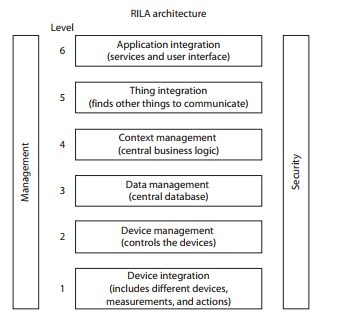
\includegraphics[scale=1.5]{images/iotrm3.png}
\centering
\caption{Γραφική απεικόνιση της πρότυπης αρχιτεκτονικής \en{IoT} εφαρμογών \cite{iotrm}}.
\label{iotrm}
\end{figure}
Έχουν γίνει πολλές προσπάθειες για να δημιουργηθούν πρότυπα μοντέλα και αρχιτεκτονικές για την ανάπτυξη εφαρμογών \en{IoT}.
Μια από τις κυρίαρχες αρχιτεκτονικές, η \en{RILA (Reference IoT Layered Architecture)}, αποδίδεται γραφικά στο Σχήμα \ref{iotrm}.
Η \en{RILA} αποτελείται από 6 οριζόντια και 2 κάθετα επίπεδα, καθώς οι έννοιες της διαχείρισης και της ασφάλειας απασχολούν κάθε στάδιο της εφαρμογής.

Για την καλύτερη κατανόηση της αρχιτεκτονικής, παρατίθεται μια σύντομη περιγραφή κάθε επιπέδου. Να σημειωθεί πως αντικείμενο θεωρείται ένα οποιοδήποτε φυσικό αντικείμενο της καθημερινότητας μας, είτε πρόκειται για ένα ψυγείο, σπίτι ή ολόκληρη πόλη, ενώ συσκευή θεωρείται οποιοσδήποτε αισθητήρας ή ενεργοποιητής.
\begin{enumerate}
    \item \textbf{Ενσωμάτωση συσκευών} --- Αυτό το επίπεδο περιλαμβάνει την επικοινωνία με κάθε είδους συσκευή, αισθητήρα ή ενεργοποιητή, επικοινωνώντας με καθένα με το αντίστοιχο πρωτόκολλο, τον εντοπισμό ή διαγραφή νέων συσκευών, καθώς και την αδιάλειπτη επικοινωνία τους με τα ανώτερα στρώματα.
    \item \textbf{Διαχείριση συσκευών} --- Αυτό το επίπεδο ελέγχει τις συσκευές, καθώς έχει μια συνολική εικόνα του δικτύου. Συγκεκριμένα, περιλαμβάνει την εισαγωγή ή διαγραφή νέων συσκευών, την επικοινωνία των εντολών στους ενεργοποιητές, τον εμπλουτισμό των δεδομένων με \en{metadata} αναφορικά με το είδος του αισθητήρα από τον οποίο συλλέχθηκαν, και τέλος την προώθηση αυτών στα ανώτερα στρώματα.
    \item \textbf{Διαχείριση δεδομένων} --- Αυτό το επίπεδο μπορεί να θεωρηθεί η βάση δεδομένων της εφαρμογής, όπου τα δεδομένα που σχετίζονται με το αντικείμενο αποθηκεύονται.
    \item \textbf{Διαχείριση πλαισίου} --- Αυτό το επίπεδο ορίζει την λογική πίσω από την εφαρμογή και είναι υπεύθυνο για τα εξής:
        \begin{itemize}
            \item Ορίζει τους στόχους του αντικειμένου.
            \item Λαμβάνει και καταναλώνει το πλαίσιο άλλων αντικειμένων.
            \item Παράγει το πλαίσιο του αντικειμένου
            \item Αξιολογεί το πλαίσιο του σε σχέση με τους στόχους του.
            \item Προκαλεί ενέργειες προκειμένου να πετύχει τους στόχους του.
            \item Δημοσιεύει το πλαίσιο του για τα άλλα αντικείμενα
        \end{itemize}
    \item \textbf{Ενσωμάτωση αντικειμένων} --- Αυτό το επίπεδο είναι υπεύθυνο για τον εντοπισμό άλλων αντικειμένων και την επικοινωνία μαζί τους. Αφού 2 αντικείμενα έχουν βρεθεί, πρέπει να περάσουν μια διαδικασία εγγραφής, κατά την οποία συγκρίνονται τα σχήματα επικοινωνίας πλαισίου και ενεργειών. Αυτή η διαδικασία μπορεί να γίνει είτε κατανεμημένα είτε κεντρικά, σε ένα διαχειριστικό συστατικό. 
    \item \textbf{Ενσωμάτωση εφαρμογής} --- Αυτό το επίπεδο περιλαμβάνει την επικοινωνία του αντικειμένου με τον χρήστη, και η μορφή της καθώς και η υλοποίησή της εξαρτάται έντονα από την εφαρμογή.
\end{enumerate}
Όσον αφορά τα κάθετα επίπεδα, ζητήματα διαχείρισης και ασφάλειας δεδομένων προκύπτουν σε όλο τα επίπεδα, από τα πρωτόκολλα επικοινωνίας των συσκευών μέχρι την λήψη αποφάσεων.

\subsection{Τεχνολογίες}
Όπως αναλύθηκε παραπάνω, το \en{IoT} περιλαμβάνει τεχνολογίες και έννοιες από πολλούς άλλους τομείς. Σε αυτό το σημείο, παρουσιάζονται οι ευρέως χρησιμοποιούμενες και σημαντικές τεχνολογίες, οι οποίες αποτελούν την βάση πολλών \en{IoT} εφαρμογών.
\subsubsection{\en{Radio frequency identification (RFID)}}
Η ταυτοποίησή ανθρώπων και αντικείμενων μέσα σε ένα κατανεμημένο δίκτυο αποτελεί βασική προϋπόθεση για οποιαδήποτε εφαρμογή \en{IoT}. Στις περισσότερες εφαρμογές χρησιμοποιούνται ετικέτες \en{RFID (RFID tags)}, οι οποίες επιτρέπουν την απόδοση ενός μοναδικού προσδιοριστικού σε όποιο αντικείμενο είναι ενσωματωμένα. Μια ετικέτα \en{RFID} είναι ένας μικρός επεξεργαστής, ο οποίος εκτελεί την στοιχειώδη λειτουργία του να μεταδίδει δεδομένα σε τυχόν ερωτήσεις από μια συσκευή ανάγνωσης (\en{RFID reader}).
\par
Υπάρχουν 3 ειδών ετικέτες \en{RFID}, ανάλογα με την πηγή ενέργεια τους.
Στην πρώτη κατηγορία ανήκουν οι ``παθητικές`` ετικέτες \en{RFID}, οι οποίες δεν περιέχουν κάποια πηγή ενέργειας, αλλά εκμεταλλεύονται την ενέργεια του λαμβανόμενου σήματος για να αποστείλουν τα απαραίτητα δεδομένα, όπως απεικονίζεται στο Σχήμα \ref{passRFID}.
Για αυτόν τον λόγο, συνήθως έχουν μικρό μέγεθος και χαμηλό κόστος.
\begin{figure}[h!]
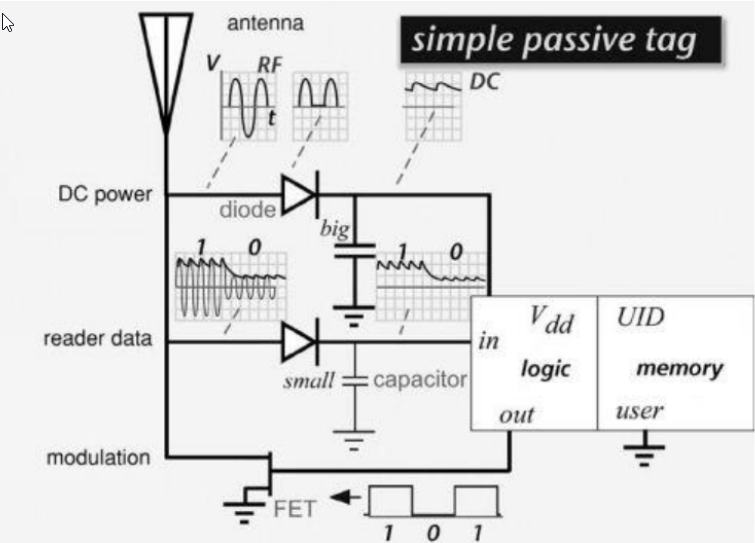
\includegraphics[scale=0.7]{images/pass_RFID.png}
\centering
\caption{Σχηματική απεικόνιση μιας ``παθητικής`` ετικέτας \en{RFID}\cite{rfidpass}.}
\label{passRFID}
\end{figure}
Στην δεύτερη κατηγορία ανήκουν οι ``ήμι-παθητικές`` ετικέτες, οι οποίες έχουν μπαταρία, αλλά την χρησιμοποιούν μόνο για την λειτουργία τους σε περίπτωση ερώτηση από συσκευή ανάγνωσης.
Τέλος, στην τρίτη κατηγορία ανήκουν οι ``ενεργητικές`` ετικέτες, οι οποίες έχουν μπαταρία και περιοδικά μεταδίδουν την πληροφορία τους και έτσι μπορούν να υποκινήσουν την επικοινωνία με μια συσκευή ανάγνωσης.
Προφανώς, οι ετικέτες που περιέχουν πηγή ενέργειας είναι μεγαλύτερες σε μέγεθος και έχουν υψηλότερο κόστος σε σχέση με τις ``παθητικές``.
\par
Οι ιδιότητες των συστημάτων \en{RFID}, που τα καθιστούν θεμέλιο λίθο του \en{IoT} είναι οι εξής:
\begin{itemize}
    \item \textbf{Μικρό μέγεθος} --- Οι μικρότερες ετικέτες \en{RFID} έχουν μέγεθος της τάξεως του 1\(mm^2\) \cite{smalltag}, οπότε υπάρχει η δυνατότητα ενσωμάτωσης σε κάθε είδους φυσικό αντικείμενο.
    Προφανώς, υπάρχει γραμμική σχέση μεταξύ του μεγέθους και της εμβέλειας της ετικέτας, οπότε η επιλογή της ετικέτας εξαρτάται από το είδος της εφαρμογής.
    \item \textbf{Χαμηλό κόστος} --- Οι φθηνότερες ετικέτες \en{RFID} κοστίζουν λιγότερο από 0.10€.
    \item \textbf{Μοναδικός τρόπος ανίχνευσης} --- Οι ετικέτες \en{RFID} εκπέμπουν έναν μοναδικό σειριακό αριθμό, οπότε επιτρέπουν την ταυτοποίηση ενός αντικείμενου από άλλα παρόμοια αντικείμενα.
    \item \textbf{Αυτοματοποίηση} --- Η διαδικασία ταυτοποίησης γίνεται αυτόματα από την συσκευή ανάγνωσης. Ενδεικτικά, μια συσκευή ανάγνωσης μπορεί να διαβάσει μέχρι και 300 ετικέτες το δευτερόλεπτο \cite{rainrfid}.
\end{itemize}

\subsubsection{Πρωτόκολλα επικοινωνίας}
Όπως είναι σαφές από την αρχιτεκτονική της, μια εφαρμογή \en{IoT} στηρίζεται στην επικοινωνία μεταξύ πολλών, ετερογενών οντοτήτων.
Το λογισμικό, το οποίο φροντίζει για την τήρηση αυτών των πρωτοκόλλων, ονομάζεται \en{middleware}.
Η αφαίρεση αυτής της πολύπλοκης διαδικασίας επιτρέπει την γρήγορη ανάπτυξη νέων εφαρμογών και την αντίστοιχα γρήγορη ενσωμάτωση παλαιότερων.
Το \en{RFC 7452} \cite{rfc7452} συνοψίζει 4 πρότυπα επικοινωνίας που χρησιμοποιούνται σε \en{IoT} εφαρμογές.
\begin{itemize}
    \item \textbf{\en{Device-to-device}} --- Πρόκειται για την περίπτωση άμεσης επικοινωνίας 2 συσκευών, συνήθως ασύρματα.
    Ανάλογα με την εφαρμογή και τις συσκευές, χρησιμοποιούνται άλλα πρωτόκολλα.
    Αυτά περιλαμβάνουν το \en{Bluetooth} ή \en{6LoWPAN}, \en{IPv6}, \en{UDP} και \en{CoAP}.
    \item \textbf{\en{Device-to-cloud}} --- Πρόκειται για την περίπτωση μεταφοράς δεδομένων από την συσκευή σε ένα σύστημα επεξεργασίας και αποθήκευσης, συνήθως στο \en{Cloud}. Η επικοινωνία βασίζεται στο \en{IP}.
    \item \textbf{\en{Device-to-gateway}} --- Πρόκειται για την περίπτωση στις οποίες το σύστημα περιλαμβάνει συσκευές που δεν μπορούν να συνδεθούν άμεσα στο Διαδίκτυο. Σε αυτές τις περιπτώσεις χρησιμοποιείται ένας εξυπηρετητής, ο οποίος παρεμβάλλεται μεταξύ των συσκευών και του Διαδικτύου. Ο εξυπηρετητής αυτός θα πρέπει να είναι σε θέση να επικοινωνεί με τις συγκεκριμένες συσκευές.
    \item \textbf{\en{Backend data sharing}} --- Πρόκειται για την περίπτωση μεταφοράς δεδομένων για να γίνει κεντρική ανάλυση. Αυτή η περίπτωση περιλαμβάνει την μεταφορά δεδομένων μεταξύ εφαρμογών \en{IoT}.
\end{itemize}
\par
Στον Πίνακα \ref{iotcomm} αναφέρονται μερικές από τις πιο διαδεδομένες τεχνολογίες επικοινωνίας και τα χαρακτηριστικά τους.
\begin{table}[h!]
    \footnotesize
    \centering
    \begin{tabularx}{\textwidth}{>{\hsize=.4\hsize}X >{\hsize=.75\hsize}X >{\hsize=.7\hsize}X X}
        Όνομα&Συχνότητα&Εμβέλεια&Εφαρμογές
        \\
        \hline
        \en{BLE}&2.4 \en{GHz}&1-100 μ.& Ακουστικά, \en{wearables}, εφαρμογές υγείας, εφαρμογές αυτοβιομηχανίας, αισθητήρες εγγύτητας, κτλπ.
         \\
         \en{EnOcean}&315, 868, 902 \en{MHz}&\(>100\) μ.& Παρακολούθηση και έλεγχος συστημάτων και αυτοματισμών, μεταφορές και \en{logistics}
         \\
         \en{GSM}&900 \en{MHz} και 1.8 \en{GHz}&30 - 300 μ.& Κινητά τηλέφωνα, παρακολούθηση στόχων, M2M
         \\
         \en{LoRa}& \(< 1\) \en{GHz ISM} μπάντα&2-45 χλμ. (ανάλογα με το περιβάλλον)& Εφαρμογές μακριάς εμβέλειας, μητροπολιτικές, M2M
         \\
         \en{NB-IoT}&700-900 \en{MHz}&10-15 χμ.& Βιομηχανική παρακολούθηση, ``έξυπνα`` σπίτια, ``έξυπνες`` πόλεις, ανίχνευση γεγονότων
         \\
         \en{NFC}& 13.56 \en{MHz}& \(< 0.2\) μ. & Διαχείριση πρόσβασης, ``έξυπνες`` κάρτες, ``έξυπνα`` πορτοφόλια
         \\
         \en{NWave}& \(< 1\) \en{GHz ISM} μπάντα&\(< 10\) χλμ.& Γεωργικές και περιβαλλοντικές εφαρμογές, εφοδιαστική αλυσίδα, ``έξυπνες`` πόλεις
         \\
         \en{RFID}& 120-150 \en{kHz (LF)}, 13.56 \en{MHz (HF)}, 865-868 \en{MHz (UHF)}, 2.4-10 \en{GHz} (μικροκύματα) &10 εκ. - 200 μ.& Διόδια, εφοδιαστική αλυσίδα, παρακολούθηση και καταγραφή αγαθών, διαχείριση πρόσβασης
         \\
        \en{SigFox}&900 \en{MHz}&3-50 χλμ. (ανάλογα με το περιβάλλον)& Εφαρμογές ασφαλείας και απομακρυσμένης παρακολούθησης
         \\
        \en{Weightless}&470-790 \en{MHz}&\(< 10\) χλμ.& Βιομηχανική παρακολούθηση, αισθητήρες κίνησης
         \\
        \en{Wi-Fi}&2.4 \en{GHz}, 3.6 \en{GHz}, 4.9/5 \en{GHz}&\(< 100\) μ.& Διακομιστές, κινητά τηλέφωνα, προσωπικοί υπολογιστές
         \\
        \en{Z-Wave}&865-926 \en{MHz}&100 μ.& Παρακολούθηση και έλεγχος ``έξυπνων`` σπιτιών και εμπορικών καταστημάτων
        \\
        \en{ZigBee}&868 \en{MHz}, 2.4 \en{GHz}&10-20 μ.& βιομηχανικός έλεγος, αυτοματισμοί σπιτιών και κατασκευών, \en{WSN}
    \end{tabularx}
    \caption{Δημοφιλή πρωτόκολλα επικοινωνίας}
    \label{iotcomm}
\end{table}

\subsubsection{\en{Cloud Computing}}

Οι \en{IoT} εφαρμογές απαιτούν επεξεργασία και αποθήκευση ετερογενών και μη σταθερών ροών δεδομένων.
Αυτήν, ακριβώς, την ανάγκη καλύπτει ο κλάδος του \en{Cloud computing}, ο οποίος παρέχει πρόσβαση σε υπολογιστικές υποδομές ή λογισμικό, τα οποία προσαρμόζονται ανάλογα με τις ανάγκες και την ζήτηση.
\par
Σύμφωνα με αρκετές οπτικές \cite{iotcloud1}\cite{iotcloud2}, τα 2 πεδία είναι συμπληρωματικά, καθώς οι \en{IoT} εφαρμογές προσφέρουν την κατανεμημένη παρουσία και τα δεδομένα από το φυσικό περιβάλλον, ενώ οι \en{Cloud} εφαρμογές προσφέρουν τους πόρους και τις υπηρεσίες που υπολείπονται οι \en{IoT} συσκευές.
Συγκεκριμένα, οι υπηρεσίες που προσφέρει το \en{Cloud} ομαδοποιούνται σε 3 κατηγορίες.
\begin{itemize}
    \item \textbf{Επικοινωνία} --- Το \en{Cloud} καθιστά δυνατή και φθηνή, την σύνδεση, παρακολούθηση και διαχείριση αντικειμένων εξ αποστάσεως, καθώς και την αυτοματοποίηση αυτών των διαδικασιών.
    \item \textbf{Αποθήκευση} --- Το \en{Cloud} καθιστά δυνατή και φθηνή, την συλλογή, αποθήκευση, συσσωμάτωση, ενσωμάτωση και, τέλος, την ομογενοποίηση των ετερογενών ροών δεδομένων, τα οποία παράγουν τα διάφορα αντικείμενα.
    \item \textbf{Επεξεργασία} --- Το \en{Cloud} καθιστά δυνατή την κεντρική, σύγχρονη και επεκτάσιμη επεξεργασία, η οποία είναι αδύνατη με τους περιορισμούς πόρους των \en{IoT} συσκευών.
\end{itemize}
\par

\subsection{Προκλήσεις}
Το \en{IoT}, ωστόσο, είναι ένας απότομα αναδυόμενος τομέας.
Οι υποδομές και, κυρίως, οι διαδικασίες που το συνθέτουν είναι ακόμα υπό διαμόρφωση.
Η πρώτη δεκαετία ανάπτυξης και εδραίωσης του \en{IoT} ανέδειξε κρίσιμα ερωτήματα και προβληματισμούς για το μέλλον του, μερικοί από τους οποίους αναφέρονται παρακάτω.
\subsubsection{Ασφάλεια}
Σαν δομικό στοιχείο κάθε δικτύου, η ασφάλεια αποτελεί ένα από τα μεγαλύτερα εμπόδια για την πλήρη ανάπτυξη του \en{IoT} \cite{foster}.
Η αλματώδης αύξηση του αριθμού και της ποικιλίας των, συνδεδεμένων στο διαδίκτυο, συσκευών αυξάνει τις πιθανές απειλές στην ασφάλεια των χρηστών.

Λόγω της έμφυτης ετερογένειας του \en{IoT}, δεν υπάρχει μια τυποποιημένη λύση για την ασφάλεια των εφαρμογών του, αλλά ορισμένοι κοινοί στόχοι.
\begin{itemize}
    \item \textbf{Εμπιστευτικότητα} --- Η πρόσβαση σε δεδομένα θα γίνεται μόνο από εξουσιοδοτημένα άτομα. Η εμπιστευτικότητα των δεδομένων είναι ιδιαίτερα σημαντική στις εφαρμογές που διαχειρίζονται ευαίσθητα προσωπικά δεδομένα.
    \item \textbf{Ακεραιότητα} --- Μια \en{IoT} εφαρμογή ή συσκευή πρέπει να διατηρεί την ακρίβεια, την συνέπεια και την αξιοπιστία των δεδομένων που αποθηκεύουν ή διαχειρίζονται. Πολύ συχνά, οι \en{IoT} συσκευές περιέχουν ευαίσθητα δεδομένα, και οποιαδήποτε μη εξουσιοδοτημένη αλλαγή σε αυτά μπορεί να έχει τεράστιες επιπτώσεις στους χρήστες.
    \item \textbf{Διαθεσιμότητα} --- Ένα \en{IoT} σύστημα ή υπηρεσία οφείλει να είναι διαθέσιμη στους εξουσιοδοτημένους χρήστες. Επιπλέον, οι χρήστες αυτοί πρέπει να έχουν πρόσβαση στα δεδομένα που τους αντιστοιχούν. Οι \en{IoT} εφαρμογές, οφείλουν να προστατεύουν τα δεδομένα και τα συστήματα τους είτε από κακόβουλες ενέργειες είτε απο αστοχίες υλικού ή λογισμικού.
\end{itemize}
\subsubsection{Δια-λειτουργικότητα}
Ήδη, έχουμε μιλήσει αρκετά για τα διάφορα προβλήματα που προκαλεί ο υψηλός βαθμός ετερογένειας που εμφανίζει το \en{IoT}.
Η ανάπτυξη μιας εφαρμογής \en{IoT} απαιτεί την διαχείριση ενός έντονα δυναμικού κατανεμημένου συστήματος, το οποίο αποτελείται από πολλές και ποικίλες συσκευές.
Η χρήση και εδραίωση μιας πρότυπης \en{IoT} αρχιτεκτονικής θα επιτρέψει την κανονικοποιήση της διαδικασίας ανάπτυξης εφαρμογών, ενώ ο περαιτέρω έλεγχος και ανάπτυξη των απαραίτητων πρωτοκόλλων επικοινωνίας θα απλοποιήσει τα ζητήματα συνδεσιμότητας των συσκευών.
\subsubsection{Επεκτασιμότητα και αξιοποίηση δεδομένων}
Καθώς το δίκτυο των διασυνδεδεμένων συσκευών θα μεγαλώνει, οι απαιτήσεις από τις υποδομές θα αυξάνονται επίσης.
Ενώ τα ζητήματα επεκτασιμότητας του δικτύου θεωρούνται διαχειρίσιμα \cite{borgia2014}, δεν ισχύει το ίδιο για τις υποδομές που διαχειρίζονται δεδομένα.
Το μέγεθος των παραγόμενων δεδομένων δεν επιτρέπει την αποθήκευση τους σε μια κεντρική βάση δεδομένων, ενώ η μεταφορά τους απαιτεί απαγορευτικές ποσότητες υπολογιστικών πόρων.
Η λύση σε αυτά τα προβλήματα απαιτεί την χρήση και την ανάπτυξη νέων \en{Cloud} εφαρμογών, που θα επιτρέπουν την κατανεμημένη αποθήκευση και επεξεργασία δεδομένων.
Πέρα από την διαχείριση των δεδομένων, προκύπτει και το ζήτημα της αξιοποίησης τους.
Η χρήση και η ανάπτυξη νέων τεχνικών εξόρυξης δεδομένων γίνεται απαραίτητη, λόγω του μεγέθους και της έλλειψης δομής των δεδομένων.
\subsubsection{Αξιοποίηση των δυνατοτήτων του \en{IoT}}
Η εξέλιξη και η ανάπτυξη των προϊόντων και των τεχνολογιών, που απαρτίζουν το \en{IoT}, κινούνται με πολύ γρήγορο ρυθμό, συγκριτικά με άλλους κλάδους. 
Αυτό συμβαίνει καθώς το \en{IoT} αποτελεί ένα προσοδοφόρο έδαφος για την ανάπτυξη νέων προϊόντων μαζικής παραγωγής αλλά και νέων επιχειρηματικών τομέων, με μεγάλο περιθώριο κέρδους. 
Αυτό οδηγεί στην ανάπτυξη μεγάλου πλήθους προϊόντων, τα οποία δεν είναι επαρκώς ελεγμένα, και είναι διάτρητα από την οπτική της ασφάλειας και της ιδωτικότητας. 
Ταυτόχρονα, αναπτύσσονται ανταγωνιστικά μοντέλα και πρότυπα επικοινωνίας και ανάπτυξης εφαρμογών, τα οποία καθιστούν το \en{IoT} ιδιαίτερα κλειστό, με τις εφαρμογές του να είναι ελάχιστα επεκτάσιμες ή επαναχρησιμοποιήσιμες. 
\subsection{Εφαρμογές}
Όπως είναι σαφές από τα παραπάνω, το \en{IoT} μπορεί να εφαρμοστεί σε πολλούς υπάρχοντες κλάδους, με σκοπό την επέκταση των δυνατοτήτων τους και την σύνδεση τους με τον ψηφιακό κόσμο.
Επίσης, επιτρέπει την μείωση του κόστους και την αύξηση της ποιότητας και της αξιοπιστίας των παρεχομένων υπηρεσιών. 
Ωστόσο, η ανάπτυξη του \en{IoT}, κυρίως, θα παράξει νέους τομείς και υπηρεσίες.
\par
Παρακάτω, παρατίθενται οι τομείς και οι εφαρμογές, οι οποίοι θα επηρεαστούν περισσότερο από την ανάπτυξη του \en{IoT}, καθώς και μια σχηματική απεικόνιση της διείσδυσης του \en{IoT} στην καθημερινότητα (Σχήμα \ref{iotapp}).
\begin{figure}[h!]
\centering
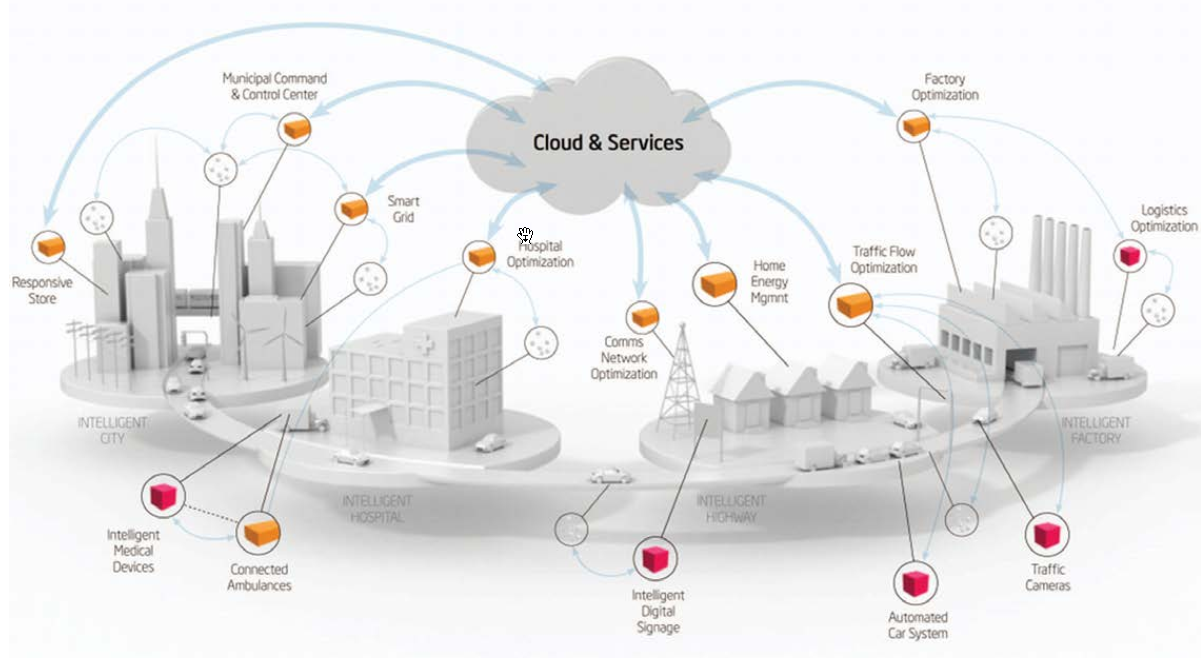
\includegraphics[scale=0.6]{images/iot_applications.png}
\caption{Σχηματική απεικόνιση των εφαρμογών του \en{IoT} \cite{iot_applications}}.
\label{iotapp}
\end{figure}

\subsubsection{Βιοϊατρική}
Οι εφαρμογές του \en{IoT} στον τομέα της Υγείας είναι πολλές και ποικίλες και αποτελούν το κύριο θέμα αυτής της διπλωματικής εργα. Θα αναφερθούμε εκτενέστερα στην ενότητα \ref{biomed} για τις εφαρμογές του \en{IoT} στον συγκεκριμένο τομέα.
\subsubsection{Μεταφορές και εφοδιαστική αλυσίδα}
Η χρήση αισθητήρων, ενεργοποιητών και επεξεργαστών επιτρέπει τον πιο ακριβή έλεγχο και χειρισμό των μεταφορικών μέσων, των μεταφερόμενων αγαθών, αλλά και της αντίστοιχης υποδομής, όπως οι δρόμοι, οι σταθερές τροχιές και οι αποθήκες διαχείρισης αγαθών.
Παρακάτω, αναφέρονται συγκεκριμένες εφαρμογές του \en{IoT} στον τομέα.
\begin{itemize}
    \item \textbf{Εφοδιαστική αλυσίδα} --- Η χρήση τεχνολογιών \en{RFID} και \en{NFC} επιτρέπουν την παρακολούθηση σε πραγματικό χρόνο κάθε κρίκου της εφοδιαστικής αλυσίδας, από τον σχεδιασμό των εμπορευμάτων και την παραγωγή μέχρι την διανομή και πώληση των προϊόντων.
    Αυτό, οδηγεί, στην ευελιξία της εφοδιαστικής αλυσίδας και την δυνατότητα προσαρμογής της σε πολύπλοκες και δυναμικές αγορές.
    \item \textbf{Υποβοηθούμενη οδήγηση} --- Εφαρμογές \en{IoT} μπορούν να παρέχουν πληροφορίες στους οδηγούς και επιβάτες των οχημάτων για καλύτερη πλοήγηση και ασφάλεια. Χαρακτηριστικές εφαρμογές είναι η διαχείριση της κυκλοφορίας των οχημάτων στους δρόμους, είτε αφορά σχεδιαστικούς σκοπούς είτε αφορά την πιο ασφαλή και γρήγορη πλοήγηση εμπορευμάτων.
    \item \textbf{Παρακολούθηση περιβαλλοντολογικών δεικτών} --- Η ασφαλής μεταφορά τροφίμων απαιτεί την τήρηση αυστηρών κανονισμών για την διατήρηση της ποιότητας τους.
    Συνήθως, αυτοί απαιτούν τις συνθήκες συντήρησης των τροφίμων να είναι συγκεκριμένες, με αυστηρά όρια στην θερμοκρασία και στην υγρασία του χώρου μεταφοράς. Η χρήση αισθητήρων επιτρέπουν την απρόσκοπτη παρακολούθηση των συνθηκών μεταφοράς τροφίμων.
\end{itemize}

\subsubsection{Έξυπνα περιβάλλοντα}
Ένα "έξυπνο περιβάλλον" είναι σε θέση να λαμβάνει πληροφορίες και να ενεργεί ανάλογα με αυτές, μέσω των αντικειμένων που το αποτελούν, διευκολύνοντας τους χρήστες του να επιτύχουν τους σκοπούς τους. Αυτός ο ορισμός περιλαμβάνει πολλές και ποικίλες χρήσεις, κάποιες από τις οποίες αναφέρονται παρακάτω. 
\begin{itemize}
    \item \textbf{Κατοικία και εργασιακοί χώροι} --- Η χρήση των δυνατοτήτων του \en{IoT} είναι σε θέση να μειώσει το κόστος και το περιβαλλοντολογικό αντίκτυπο της οικιστικής και επαγγελματικής χρήσης των κτηρίων\cite{iothome}. Ταυτόχρονα, η αυτοματοποίηση των διαδικασιών ελέγχου και παρακολούθησης, οδηγεί στην βελτίωση των συνθηκών ασφαλείας καθώς και την πιο άνετη διαβίωση των κατοίκων/υπαλλήλων.
    \item \textbf{Βιομηχανική και αγροτική παραγωγή} --- Οι εφαρμογές \en{IoT}, ήδη, διαδραματίζουν μεγάλο ρόλο στην βιομηχανία \cite{iotmanuf} και στην γεωργία \cite{iotagric}, καθώς καθιστούν δυνατή την περαιτέρω αυτοματοποίηση της παραγωγής.
    Συγκεκριμένα, στην βιομηχανική παραγωγή, οι δυνατότητες του \en{IoT} επιτρέπουν την βελτιστοποίηση της παραγωγής, τον άμεσο εντοπισμό και διόρθωση σφαλμάτων καθώς και την διαχείριση του εργασιακού περιβάλλοντος.
    Ταυτόχρονα, στην αγροτική παραγωγή, επιτρέπουν τον έλεγχο της άρδευσης, την παρακολούθηση των περιβαλλοντικών συνθηκών, των εντόμων και των άλλων ζώων που επηρεάζουν την παραγωγή.
    \item \textbf{Πόλεις} --- Η χρήση των δυνατοτήτων του \en{IoT} επιτρέπει, πλέον, την παρακολούθηση των υπηρεσιών και των συνθηκών μιας πόλης σε πραγματικό χρόνο.
    Αυτές ποικίλουν από την διαχείριση της κυκλοφορίας των οχημάτων μέχρι την διαχείριση κοινωφελών αγαθών, όπως η συγκομιδή απορριμάτων και η ύδρευση.
    Ιδιαίτερο ενδιαφέρον, παρουσιάζουν οι εφαρμογές που σχετίζονται με το \en{CIM (City Information Model)} \cite{iotcity}.
    Πρόκειται για την ιδέα ενός αστικού ιστού, πλήρως διασυνδεδεμένου, που επιτρέπει την παρακολούθηση και έλεγχο κάθε συστατικού του στοιχείου, είτε αυτό πρόκειται για κτήρια είτε πρόκειται για υποδομές, όπως το ηλεκτρικό δίκτυο.
\end{itemize}
\begin{comment}{}
\section{Μηχανική Μάθηση}
\subsection{Εισαγωγή}
Την τελευταία δεκαετία, η Μηχανική Μάθηση, όπως το \en{Internet of Things}, αποτέλεσε έναν τεχνολογικό κλάδο με εκρηκτική ανάπτυξη και δυσανάλογα υψηλές προσδοκίες.
Η Μηχανική Μάθηση είναι ένα υπολογιστικό πεδίο της Τεχνητής Νοημοσύνης. 
Αντικείμενο του είναι η κατασκευή συστημάτων αυτόματης μάθησης και βελτιστοποίησης, χωρίς σαφείς κανόνες για τον υπολογισμό ή την λύση προβλημάτων.
Στην βάση της μηχανικής μάθησης υπάρχει η υπόθεση ότι \textit{η γνώση μπορεί να προκύψει από τα δεδομένα.}
\par
Οι αλγόριθμοι μηχανικής μάθησης βασίζονται σε ένα σύνολο δεδομένων εισόδου, το οποίο ονομάζεται σύνολο εκπαίδευσης.
Αυτό αποτελείται από παραδείγματα της εισόδου του τελικού συστήματος ή εμπειρικά αποτελέσματα του συστήματος προς προσομοίωση.
Το σύνολο εκπαίδευσης χρησιμοποιείται για την αναγνώριση επαναλαμβανόμενων προτύπων στα δεδομένα και να οδηγήσει σε καλύτερες αποφάσεις στο μέλλον.
\par
Οι αλγόριθμοι μηχανικής μάθησης διακρίνονται σε 2 κατηγορίες, με κριτήριο τον τρόπο μάθησης, δηλαδή το πως δίνεται ανάδραση στο αναπτυσσόμενο σύστημα.
Δύο από τις ευρέως υιοθετούμενες μεθόδους μηχανικής μάθησης είναι η \textit{επιβλεπόμενη μάθηση} και η \textit{μη επιβλεπόμενη μάθηση}.
Η πρώτη απαιτεί την επισήμανση των παρατηρήσεων του συνόλου εκπαίδευσης με το επιθυμητό αποτέλεσμα του τελικού συστήματος, ενώ η δεύτερη δεν χρειάζεται την πληροφορία αυτή.
\subsection{Επιβλεπόμενη μάθηση}
Η επιβλεπόμενη μάθηση χρησιμοποιείται για την εκμάθηση της συνάρτησης απεικόνισης \(f\) από μερικές μεταβλητές εισόδου \(X\) σε μια μεταβλητή εξόδου \(Y\).
\begin{equation}
  Y = f(X)  
\end{equation}
Ο σκοπός της επιβλεπόμενης μάθησης είναι να προσεγγίσει την δομή της συνάρτησης απεικόνισης, έτσι ώστε να μπορεί να γενικεύσει και να προβλέπει σωστά το αποτέλεσμα καινούργιων παρατηρήσεων. 
Η διαδικασία μάθησης περιλαμβάνει την επαναλαμβανόμενη πρόβλεψη των αποτελεσμάτων των δεδομένων εισόδου, την σύγκριση με τις γνωστές, σωστές απαντήσεις και την διόρθωση των παραμέτρων του εκάστοτε μοντέλου.
Η διαδικασία αυτή σταματά όταν επιτευχθεί κάποιο κριτήριο, το οποίο συνήθως είναι αριθμός επαναλήψεων ή κάποιο κριτήριο απόδοσης.
Η χρήση επιβλεπόμενης μάθησης χρησιμοποιείται συνήθως σε προβλήματα \textit{παλινδρόμησης \en{(regression)}} και σε προβλήματα  \textit{ταξινόμησης \en{(classification)}}.
Η μεταβλητή εξόδου στα προβλήματα παλινδρόμησης είναι συνεχής, ενώ, αντίθετα, στα προβλήματα ταξινόμησης είναι διακριτή.
\subsection{Μη επιβλεπόμενη μάθηση}
Αντίθετα, η μη επιβλεπόμενη μάθηση, λόγω της έλλειψης επισήμανσης των παραδειγμάτων εισόδου, βασίζεται στον εντοπισμό μοτίβων.
Μια βασική κατηγορία προβλημάτων, στα οποία εφαρμόζεται η μη επιβλεπόμενη μάθηση, είναι η \textit{ομαδοποίηση \en{(clustering)}}.
Σκοπός αυτών των προβλημάτων, είναι η ομαδοποίηση παρατηρήσεων, έτσι ώστε τα μέλη μιας ομάδας να είναι παρόμοια μεταξύ τους, και να διαφέρουν σημαντικά από τα μέλη των άλλων ομάδων.
Άλλη κατηγορία προβλημάτων, που βρίσκει εφαρμογή η μη επιβλεπόμενη μάθηση, είναι τα \textit{γεννητικά μοντέλα \en{(generative models)}}.
Τα μοντέλα αυτά μιμούνται την διαδικασία δημιουργίας των δεδομένων εκπαίδευσης.
Σκοπός τους είναι η δημιουργία νέων τεχνητών δεδομένων, τα οποία να είναι παρόμοια με τα αυθεντικά.
\subsection{Δημοφιλή μοντέλα μηχανικής μάθησης}
Στα πλαίσια αυτής της διπλωματικής εργασίας, παρουσιάζονται ορισμένες βασικές έννοιες και μερικά δημοφιλή μοντέλα, τα οποία χρησιμοποιήθηκαν.
\subsubsection{Συνάρτηση κόστους}
Ο στόχος κάθε αλγορίθμου επιβλεπόμενης μάθησης είναι να προσεγγίσει 

\end{comment}
\newpage
\section{\en{Internet of Things} και Βιοϊατρική}\label{biomed}
\subsection{Εισαγωγή}
Η εξέλιξη της ιατρικής τεχνολογίας, καθώς και η αύξηση της αγροτικής παραγωγής έχει προκαλέσει την αύξηση του πληθυσμού, καθώς και την αύξηση του προσδόκιμου ζωής, όπως φαίνεται στο σχήμα \ref{human_population}.
Αντίθετα σε αυτήν την κατάκτηση της ανθρωπότητας, πολλά εκατομμύρια ανθρώπων ζουν σε δριμέα περιβάλλοντα, τα οποία χαρακτηρίζονται από την έλλειψη πόσιμου νερού και άλλων απαραίτητων υποδομών.
Ταυτόχρονα, συχνές είναι οι εξάρσεις επιδημιών, ενώ η κλιματική αλλαγή ήδη επηρεάζει το περιβάλλον και την υγεία των κατοίκων των παθόντων περιοχών.
Τέλος, η αύξηση του προσδόκιμου ζωής έρχεται σε αντίθεση με τις συνθήκες κατά τις οποίες σχεδιάστηκαν τα προϋπάρχοντα συστήματα κοινωνικής ασφάλισης στον δυτικό κόσμο, οδηγώντας συχνά σε υποβαθμισμένη διαβίωση για τους ηλικιωμένους ή για άτομα με ειδικές ανάγκες.
\begin{figure}[h!]
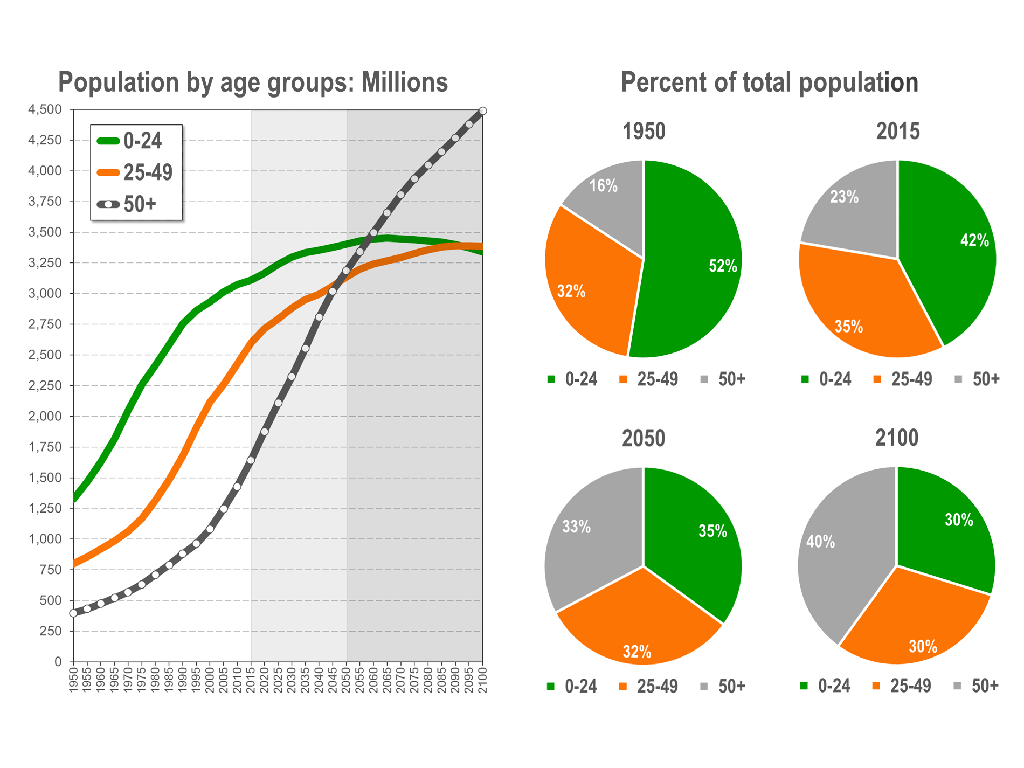
\includegraphics[scale=0.4]{images/human_population.png}
\centering
\caption{Σχηματική απεικόνιση της εξέλιξης του ανθρώπινου πληθυσμού και της ηλικιακής σύνθεσης του. \cite{human_population}}
\label{human_population}
\end{figure}
Είναι σαφές πως η ζήτηση για ποιοτικές υπηρεσίες υγείας έχει αυξηθεί και θα συνεχίσει να αυξάνεται, κυρίως λόγω της αύξησης του πληθυσμού. \cite{Lubitz2003} 
Εξίσου σαφές είναι το γεγονός ότι τα υπάρχοντα συστήματα και μοντέλα παροχής υπηρεσιών υγείας συχνά κρίνονται ανεπαρκή για την κάλυψη αυτής της ζήτησης, εξαιτίας της ανισότητας πρόσβασης σε αυτά, όπως φαίνεται στο γράφημα \ref{insufficient}. 
\begin{figure}[h!]
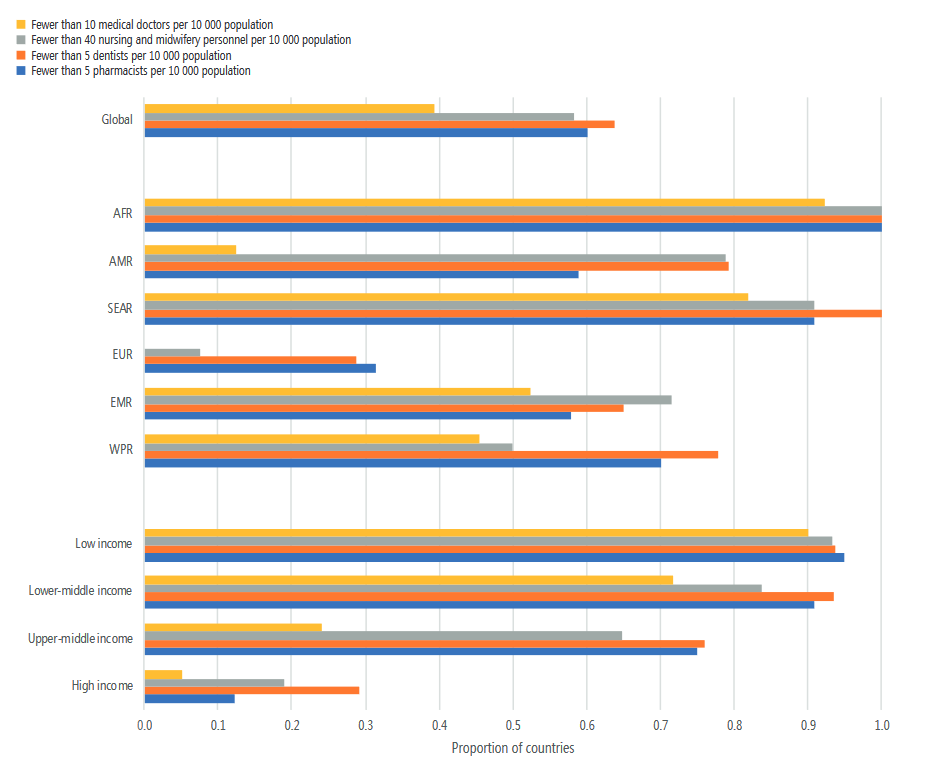
\includegraphics[scale=0.6]{images/who_insufficient.png}
\centering
\caption{Έλλειψη ιατρικού προσωπικού ανάλογα με την ήπειρο και το σχετικό μέσο εισόδημα κάθε χώρας. \cite{WHO}}
\label{insufficient}
\end{figure}
\par

Παρακάτω, αναφέρονται σύντομα ορισμένες από τις μεγαλύτερες προκλήσεις του υπάρχοντος συστήματος υγειονομικής περίθαλψης.
\begin{itemize}
    \item \textbf{Υπηρεσίες υγείας σαν εμπόρευμα} --- Η αντιμετώπιση της παροχής υπηρεσιών υγείας ως εμπόρευμα οδηγεί στην περιθωριοποίηση δαπανηρών αλλά αναγκαίων θεραπειών ή ερευνών.
    \item \textbf{Μειούμενη αναλογία ιατρικού προσωπικού ανά ασθενή} --- Ως συνέχεια του παραπάνω, η μείωση του εξειδικευμένου ιατρικού προσωπικού σε συνδυασμό με την αύξηση του πληθυσμού, οδηγεί σε χαμηλής ποιότητας υπηρεσίες υγείας.
    \item \textbf{Αστικοποίηση} --- Οι σημερινές μητροπόλεις με τα εκατομμύρια πολιτών απαιτούν συνεχείς και μεγάλες επενδύσεις στις υποδομές υγείας, κάτι το οποίο δεν είναι εφικτό ή δεν προτιμάται.
    \item \textbf{Αύξηση του προσδόκιμου ζωής} --- Τέλος, η αύξηση του προσδόκιμου ζωής αυξάνει τον αριθμό των ατόμων που επιζητούν υπηρεσίες υγείας και καθιστά αναγκαία την θεραπεία και διαχείριση χρόνιων παθήσεων.
\end{itemize}
Για την κάλυψη των συγχρόνων κοινωνικών αναγκών υγείας, απαιτείται η επιστράτευση της τεχνολογίας, καθώς και η αλλαγή του μοντέλου υγειονομικής περίθαλψης.
Συγκεκριμένα, απαιτείται να αξιοποιηθούν επικουρικά οι δυνατότητες των νέων τεχνολογιών, όπως και του \en{IoT}, δίχως την περιθωριοποίηση των αναγκών σε ιατρικό προσωπικό και υλικό.
Ταυτόχρονα, και με χρήση των παραπάνω τεχνολογιών, πρέπει να αναδειχθεί η πρόληψη σαν κύριος άξονας της δημόσιας υγείας, δίνοντας ενεργό ρόλο στον πολίτη για την διαχείριση της υγείας του.
\begin{figure}[h!]
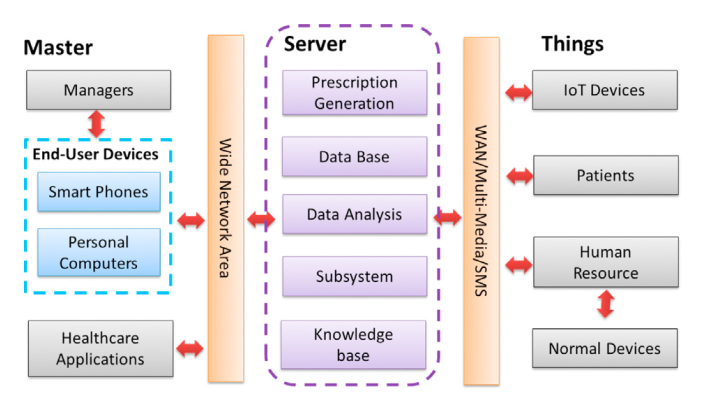
\includegraphics[scale=1]{images/iot_h_example.png}
\centering
\caption{Σχηματική απεικόνιση της αρχιτεκτονικής ενός \en{IoT} συστήματος αποκατάστασης \cite{iot_h_example}}.
\label{iot_h_example}
\end{figure}
\subsection{Λόγοι σύγκλισης}
Οι δυνατότητες των εφαρμογών \en{IoT} μπορούν να καλύψουν ορισμένα από τα προβλήματα που αναφέρθηκαν προηγουμένως. Η δομή των εφαρμογών \en{IoT} μοιάζει με την ιεραρχική δομή ενός συστήματος παροχής υπηρεσιών υγείας, όπως φαίνεται στο Σχήμα \ref{iot_h_example}, όπου βλέπουμε σχηματικά την αρχιτεκτονική ενός συστήματος αποκατάστασης, βασισμένο σε τεχνολογίες \en{IoT}.

Παρακάτω, αναφέρονται ορισμένα από τα πλεονεκτήματα που προσφέρει η χρήση \en{IoT} εφαρμογών στον τομέα της υγείας.
\begin{itemize}
    \item \textbf{Συνεχής και διακριτική καταγραφή των ζωτικών σημείων του ασθενή} ---
    Οι εξελίξεις στην τεχνολογία των βιοαισθητήρων, επιτρέπει την απρόσκοπτη καταγραφή και αποστολή βιοσημάτων από τους ασθενείς, χωρίς να χρειαστεί να αλλάξουν τις καθημερινές τους συνήθειες. Αυτό επιτρέπει την πιο ακριβή και γρήγορη διάγνωση ασθενειών, καθώς και την συλλογή μεγάλου όγκου ιατρικών δεδομένων.
    \item \textbf{Απρόσκοπτη χρήση διάφορων τεχνολογιών} ---
    Η χρήση εφαρμογών \en{IoT} επιτρέπει την χρήση πολλών τεχνολογιών, οι οποίες δεν είχαν εφαρμοστεί πρότερα στον τομέα της υγείας, εξαιτίας της δυσκολίας ενσωμάτωσης τους στις ιατρικές διαδικασίες.
    \item \textbf{Απομακρυσμένη διεπαφή ασθενή και ιατρικού προσωπικού} ---
    Οι εφαρμογές \en{IoT} επιτρέπουν την άμεση, απομακρυσμένη επικοινωνία του ασθενή με κατάλληλο ιατρικό προσωπικό, σε πραγματικό χρόνο. Το προσωπικό αυτό θα έχει άμεση πρόσβαση στα ιατρικό ιστορικό και τα δεδομένα πραγματικού χρόνου του ασθενή.
    \item \textbf{Εξατομικευμένες υπηρεσίες} ---
    Πολλές ασθένειες και παθήσεις δεν εκφράζονται με τον ίδιο τρόπο σε όλους τους ανθρώπους. Η μακρόχρονη συλλογή δεδομένων από έναν ασθενή επιτρέπει την δημιουργία ενός εκτενούς και ακριβούς ιατρικού ιστορικού. Με βάση αυτά τα δεδομένα και την χρήση τεχνικών μηχανικής μάθησης, είναι δυνατή η πρόβλεψη της κατάστασης της υγείας του ασθενή. 
    \item \textbf{Μείωση κόστους} ---
    Η βελτίωση της δυνατότητας πρόβλεψης της υγείας του πολίτη βοηθά την αποτελεσματικότερη διαχείριση του χρόνου του ιατρικού προσωπικού, αλλά και του ιατρικού υλικού.
    \item \textbf{Εύκολη χρήση} ---
    Οι εφαρμογές \en{IoT} στον τομέα της υγείας απευθύνονται και σε άτομα με ειδικές ανάγκες, καθώς και ηλικιωμένους. Οπότε, είναι σχεδιασμένες να χρησιμοποιούνται εύκολα και άμεσα από τους χρήστες τους.
    \item \textbf{Συσσώρευση ιατρικών δεδομένων} ---
    Η συλλογή, επεξεργασία και ανάλυση του τεράστιου πλήθους δεδομένων, που παράγουν οι \en{IoT} εφαρμογές, δίνει νέες δυνατότητες στην ιατρική έρευνα.
\end{itemize}
\subsection{Εφαρμογές}
Η Βιοϊατρική είναι ένας τεράστιος κλάδος, ώστε οι δυνατότητες εφαρμογής των τεχνολογιών του \en{IoT} να μοιάζουν ατέλειωτες, από την απομακρυσμένη παρακολούθηση των ασθενών μέχρι την αντιμετώπιση ασθενειών.
Η χρήση του \en{IoT} περιορίζεται, προς το παρόν, στην τηλεϊατρική και στην καταγραφή και παρακολούθηση κεφαλαίων.
\par
Παρακάτω αναφέρονται οι βασικές εφαρμογές του \en{IoT} στον τομέα της Βιοϊατρικής.
\subsubsection{Περιβάλλοντα Υποβοηθούμενης Διαβίωσης (ΠΥΔ)}
Μια από τις βασικές εφαρμοηές του \en{IoT} είναι η κατασκευή και διαχείριση έξυπνων περιβαλλόντων, τα οποία καθιστούν πιο εύκολη την ζωή των ατόμων που κινούνται μέσα σε αυτά.
Στον τομέα της Βιοϊατρικής, τα άτομα αυτά είναι ασθενείς ή ηλικιωμένοι άνθρωποι, οι οποίοι δεν μπορούν να καλύψουν τις ανάγκες τους χωρίς βοήθεια.
Τα ΠΥΔ αποτελούν βασικό αντικείμενο της διπλωματικής και για αυτό αναλύονται στο κεφάλαιο 2.
\subsubsection{\en{mHealth (mobile Health)}}
Η χρήση του \en{Cloud Computing}, μέσω \en{mobile} και \en{web} εφαρμογών, επιτρέπει την απομακρυσμένη πρόσβαση σε ιατρική πληροφορία.
Ταυτόχρονα, οι ίδιες εφαρμογές επιτρέπουν στο ιατρικό προσωπικό την παροχή οδηγιών και βοήθειας, επικοινωνώντας μέσω \en{video} με τον ασθενή.
Η συγκεντρωμένη ιατρική πληροφορία των ασθενών επιτρέπει στο ιατρικό προσωπικό να παρέχουν πιο άμεση και κατάλληλη θεραπεία για κάθε ασθενή.
\subsubsection{Διαχείριση ιατρικού υλικού}
Η χρήση ετικετών \en{RFID} επιτρέπει την πλήρη διαχείριση του ιατρικού υλικού.
Αρχικά, καθιστά πολύ δυσκολότερη την χάλκευση των ιατρικών προϊόντων, μέσω της μοναδικής ταυτότητας που παρέχει η \en{RFID} ετικέτα.
Στη συνέχεια, κάθε στάδιο της εφοδιαστικής αλυσίδας του προϊόντος καταγράφεται και η πληροφορία αυτή γίνεται διαθέσιμη στον καταναλωτή.
\par
Επίσης, η χρήση εφαρμογών \en{IoT} επιτρέπει την παρακολούθηση της σωστής λειτουργίας κρίσιμων ιατρικών συσκευών, όπως βηματοδότες ή άλλες έμφυτες συσκευές, και ενημερώνει σε πιθανή δυσλειτουργία.
Τέλος, η χρήση ετικετών \en{RFID} επιτρέπει την δημιουργία ενός διαφανούς συστήματος καταγραφής και παρακολούθησης ιατρικών αποβλήτων, σε συνεργασία με τα νοσοκομεία και μεταφορικές εταιρείες. 
\subsubsection{Ψηφιακά νοσοκομεία}
Οι τεχνολογίες που απαρτίζουν το \en{IoT} καθιστούν δυνατή την ψηφιοποίηση και αυτοματοποίηση των διοικητικών διαδικασιών ενός νοσοκομείου, καθώς και την παροχή επαυξημένων δυνατοτήτων στο ιατρικό προσωπικό.
Η σταδιακή εγκαθίδρυση των ηλεκτρονικών μητρώων υγείας, σε συνδυασμό με την χρήση ετικετών \en{RFID} επιτρέπει την άμεση ταυτοποίηση των ασθενών, καθώς και την πρόσβαση στο ιατρικό τους ιστορικό.
Για τον ίδιο λόγο, η διαχείριση ιατρικών επειγόντων περιστατικών γίνεται ευκολότερη, ενώ περαιτέρω βοηθά η διασύνδεση των οργάνων των ασθενοφόρων με το νοσοκομείο.
\par
Η καταγραφή, παρακολούθηση και αξιοποίηση του νοσοκομειακού εξοπλισμού, καθώς και του ιατρικού υλικού, γίνεται ευκολότερη και πιο ακριβής.
Για παράδειγμα, η διαχείριση της αποθήκης φαρμάκων, καθώς και η διανομή τους, μπορεί να γίνει ηλεκτρονικά, αλλά και να αυτοματοποιηθεί.
\par
Επίσης, σημαντικές αλλαγές μπορούν να συμβούν στην διαχείριση των ασθενών και της εμπειρίας τους στο νοσοκομείο.
Αρχικά, η χρήση ετικετών \en{RFID} επιτρέπει στο ιατρικό προσωπικό να έχει περισσότερο έλεγχο στην ροή των ανθρώπων.
Η συνεχής παρακολούθηση των ζωτικών σημείων των ασθενών αποτελεί την βάση ενός έξυπνου συστήματος ειδοποίησης σε περίπτωση ανάγκης.
Ταυτόχρονα, ο ασθενής είναι σε θέση να χειρίζεται το περιβάλλον νοσηλείας του, μέσω τεχνολογιών αναγνώρισης φωνής και \en{mobile} εφαρμογές.
\par
Τέλος, είναι εφικτή η βελτίωση της απόδοσης του ιατρικού προσωπικού, ιδιαίτερα στους τομείς των επειγόντων, της χειρουργικής και της ραδιολογικής.
Η παροχή των απαραίτητων πληροφοριών τους επιτρέπει να πάρουν κρίσιμες αποφάσεις γρηγορότερα και με μεγαλύτερη ακρίβεια.
\subsubsection{Απομακρυσμένη παρακολούθηση ασθενών}
Οι εξελίξεις στον τομέα των βιοαισθητήρων και η καθιέρωση του κλάδου των \en{wearables} καθιστούν δυνατή την απομακρυσμένη παρακολούθηση των ασθενών σε μη κλινικά περιβάλλοντα.
Αυτή περιλαμβάνει την συλλογή σημάτων (βιολογικών και μη) από αισθητήρες, την πιθανή καταγραφή εικόνας και ήχου και την αποστολή τους στο κατάλληλο ιατρικό προσωπικό.
Η πορεία της θεραπείας, οι προτάσεις του ιατρικού προσωπικού και το σύστημα ειδοποιήσεων παρέχονται στον ασθενή, μέσω \en{mobile} εφαρμογών.
\par
Η ένταξη της απομακρυσμένης παρακολούθησης ασθενών στην διαχείριση χρόνιων παθήσεων οδηγεί στην βελτίωση της ποιότητας ζωής των ασθενών.
Τους επιτρέπει να διατηρήσουν την ανεξαρτησία τους και να επιλύουν ευκολότερα επιπλοκές.
%\chapter{Περιβάλλοντα Υποβοηθούμενης Διαβίωσης}
\label{chap2}
\section{Εισαγωγή}
Τα Περιβάλλοντα Υποβοηθούμενης Διαβίωσης (ΠΥΔ) αποτελούν έναν αναδυόμενο διεπιστημονικό κλάδο, ο οποίος στοχεύει στην ανάπτυξη εννοιών, προϊόντων και υπηρεσιών που συνδυάζουν τεχνολογίες πληροφορικής και επικοινωνιών με κοινωνικές ανάγκες, προσφέροντας βελτιωμένη ποιότητα ζωής σε άτομα που χρήζουν υποστήριξης, ιδίως στους ηλικιωμένους.

Οι ΠΥΔ ενσωματώνουν γνώση από τους τομείς της Βιοϊατρικής, του \en{Internet of Things}, του \en{Cloud Computing}, της Μηχανικής Μάθησης και άλλων συναφών επιστημονικών περιοχών.
\par
Η συνεχής αύξηση του προσδόκιμου ζωής στη Δύση αποτελεί έναν από τους κύριους κινητήριους μοχλούς ανάπτυξης του κλάδου.
Πλέον, απαιτούνται καινοτόμες και αποδοτικές λύσεις, με ιδιαίτερη έμφαση στη πρόληψη, για την υποστήριξη αυτών των ευαίσθητων κοινωνικών ομάδων.
Συγκεκριμένα, ο σκοπός των ΠΥΔ είναι να δημιουργήσουν οφέλη σε τρεις επιπέδους: για τα \textit{άτομα}, μέσω αυξημένων δυνατοτήτων και ασφάλειας, για την \textit{οικονομία}, μέσω του περιορισμού του κόστους των υπηρεσιών υγείας, και τέλος για την \textit{κοινωνία}, μέσω της βελτίωσης της συνολικής ποιότητας ζωής. Μια σχηματική απεικόνιση των πλεονεκτημάτων αυτών φαίνεται στο Σχήμα \ref{aalpro}. 

\section{Χαρακτηριστικά}
Παρότι δεν υπάρχει ακριβής και καθολικά αποδεκτός ορισμός για τα ΠΥΔ στη διεθνή βιβλιογραφία, μελετώντας τις διάφορες προσπάθειες εννοιολογικής οριοθέτησης, μπορούμε να διατυπώσουμε τον ακόλουθο ορισμό:
\begin{quote}
    Τα Περιβάλλοντα Υποβοηθούμενης Διαβίωσης αποτελούν σύγχρονες τεχνολογικές λύσεις Πληροφορικής και Επικοινωνιών, βασισμένα στις αρχές του νοήμονος περιβάλλοντος, για την παροχή καθολικής, μη επεμβατικής και προληπτικής φροντίδας σε ηλικωμένους και σε άλλα άτομα που χρήζουν φροντίδα, με τελικό σκοπό τη διατήρηση της ανεξαρτησίας και τη βελτίωση της ποιότητας ζωής τους, καθώς και την υποστήριξη των ατόμων που τους φροντίζουν. 
\end{quote}

\begin{figure}[h!]
\centering
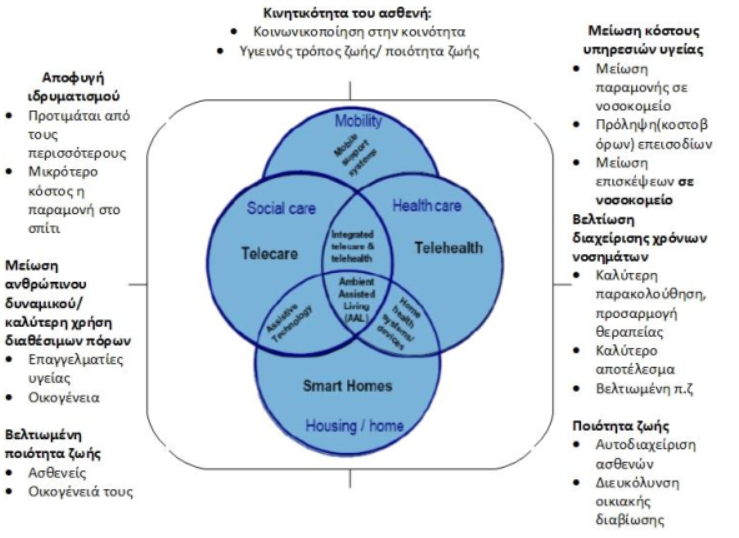
\includegraphics[scale=0.9]{images/aal.png}
\caption{Σχηματική απεικόνιση των πλεονεκτήματων των ΠΥΔ}.
\label{aalpro}
\end{figure}

Παρακάτω, θα επεξηγηθούν οι έννοιες που απαρτίζουν αυτόν τον ορισμό.

\subsection{Νοήμων περιβάλλον}
Το νοήμων περιβάλλον αποτελεί ένα ερευνητικό παράδειγμα που ενσωματώνει υπολογιστική ευφυΐα στα καθημερινά περιβάλλοντα μέσω τεχνολογιών \en{IoT}, διάχυτης υπολογιστικής και τεχνητής νοημοσύνης. Στόχος είναι η δημιουργία περιβαλλόντων ικανών να αντιλαμβάνονται, να προσαρμόζονται και να αντιδρούν στις ανθρώπινες ανάγκες \cite{Aarts2003}.

Τα ΠΥΔ εφαρμόζουν αυτό το παράδειγμα ειδικά για την υποστήριξη ηλικιωμένων, δημιουργώντας υποβοηθητικές τεχνολογίες με τα εξής χαρακτηριστικά \cite{Acampora2013}\cite{Blackman2016}:
\begin{itemize}
    \item Μη επεμβατική και απρόσκοπτη ενσωμάτωση στο περιβάλλον του χρήστη.
    \item Δράση ανάλογα με το εκάστοτε πλαίσιο και την κατάσταση του χρήστη. 
    \item Προσωποποιημένη φροντίδα για τις ανάγκες κάθε χρήστη. 
    \item Προσαρμογή στον χρήστη μέσω συνεχούς μάθησης.
    \item Προνόηση και πρόβλεψη των αναγκών και επιθυμιών του χρήστή.
\end{itemize}

Συνολικά, τα ΠΥΔ μπορούν να ειδωθούν ως το αποτέλεσμα της προόδου από τις διάφορες μεμονωμένες συσκευές, οι οποίες εξυπηρετούσαν ένα συγκεκριμένο έργο, σε ένα νοήμων περιβάλλον το οποίο θα βοηθά και υποστηρίζει τον χρήστη και τον ζωτικό του χώρο \cite{Blackman2016}.

\subsection{Σύγχρονες υπολογιστικές και επικοινωνιακές τεχνολογίες}
Τα ΠΥΔ περιλαμβάνουν ένα ευρύ φάσμα εξελιγμένων τεχνολογιών με ιδιαίτερη έμφαση στα 'έξυπνα' σπίτια, τα κινητά και ένδυτα συστήματα και την υποβοηθητική ρομποτική.\cite{rashidi2012survey}
Οι τεχνολογίες αυτές συνδυάζονται με εξελιγμένες υπολογιστικές τεχνικές, όπως η αναγνώριση ανθρώπινης δραστηριότητας, η ανακάλυψη συμπεριφορικών μοτίβων, η ανίχνευση μη ομαλών δεδομένων, η μοντελοποίηση πλαισίου, η αναγνώριση τοποθεσίας και ταυτότητας, κλπ. \cite{rashidi2012survey} \cite{Acampora2013}.
\par
Όλα τα συστατικά των ΠΥΔ είναι διασυνδεδεμένα και επικοινωνούν μεταξύ τους.
Οι ενσωματωμένοι αισθητήρες συλλέγουν πληροφορίες σχετικά με το περιβάλλον και τον χρήστη.
Οι υπολογιστικές τεχνικές συναθροίζουν την πληροφορία από τους επιμέρους αισθητήρες, την αναλύουν, την ερμηνεύουν και αποφασίζουν για την κατάλληλη δράση.
Τέλος, οι διάφοροι ενεργοποιητές, έξυπνες διεπαφές και υποβοηθητικές συσκευές δρουν αναλόγως και επιτρέπουν τη διάδραση με τον χρήστη \cite{broek}.
\subsection{Η ανεξαρτησία και η βελτίωση της ποιότητας ζωής των ηλικιωμένων ως σκοπός}
Το όραμα των ΠΥΔ είναι να παρέχει στους ηλικιωμένους ασφαλή και υποστηρικτικά περιβάλλοντα, να διατηρούν και να βελτιώνουν τη φυσική, πνευματική και ψυχική τους υγεία και να ενισχύουν την κοινωνική ενασχόληση και την ενεργή συμμετοχή στη κοινωνία \cite{Queiros2013}\cite{Blackman2016}\cite{broek}\cite{Peek2014}\cite{cardinaux}.
Ο απώτερος σκοπός των ΠΥΔ είναι η διασφάλιση της ανεξαρτησίας των ηλικιωμένων και η βελτίωση της ποιότητας ζωής τους.
\par
Ταυτόχρονα, η τεχνολογία των ΠΥΔ απευθύνεται και στους παρόχους φροντίδας, είτε πρόκειται για ιατρικό προσωπικό είτε για τον κοινωνικό κύκλο των ηλικιωμένων ατόμων.
Η τεχνολογία των ΠΥΔ σκοπεύει να μειώσει το βάρος των ευθυνών των παρόχων φροντίδας, να ενισχύσει το αίσθημα της σιγουριάς, να βοηθήσει στη διαχείριση και τον συντονισμό των καθηκόντων φροντίδας και, τέλος, να διευκολύνει την απομακρυσμένη επικοινωνία και την κοινωνική διασύνδεση μεταξύ των παρόχων φροντίδας και των ηλικιωμένων \cite{rashidi2012survey}\cite{Bossen2013}\cite{Cornejo2012}.
\section{Τομείς εφαρμογής}
Το όραμα της τεχνολογίας των ΠΥΔ στοχεύει στην παροχή ολιστικής υποστήριξης των χρηστών. Κατά συνέπεια, τα ΠΥΔ βρίσκουν εφαρμογή σε κάθε πτυχή της καθημερινής ζωής.
Συγκεκριμένα, έχουν εντοπιστεί 3 βασικοί τομείς εφαρμογής, όπως παρουσιάζονται παρακάτω \cite{broek}.

\subsection{Ευγηρία στο σπίτι}
Ο πρώτος τομέας περιγράφεται ως \textit{``η δυνατότητα ποιοτικότερης καθημερινότητας, για περισσότερο χρόνο, διατηρώντας υψηλό βαθμό ανεξαρτησίας, αυτονομίας και αξιοπρέπεια''} \cite{broek}.
Η πλειοψηφία των ηλικιωμένων προτιμά την παραμονή στο γνωστό οικιακό τους περιβάλλον για το μεγαλύτερο δυνατό διάστημα \cite{Mosca2016}.
Ωστόσο, η μείωση των πνευματικών και σωματικών ικανοτήτων τους, λόγω της γήρανσης του οργανισμού, καθιστά την αυτόνομη διαμονή τους περίπλοκη και απαιτητική.
Ακόμα και ηλικιωμένοι, οι οποίοι είναι υγιείς και ενεργοί, είναι πιθανό να χρειαστούν κάποια μορφή φροντίδας στο άμεσο μέλλον.
Η δημιουργία ενός ασφαλούς και υποβοηθητικού οικιακού περιβάλλοντος είναι, επομένως, ένας σημαντικός τομέας ενδιαφέροντος των ΠΥΔ.
Παραδείγματα εφαρμογών σε αυτόν τον τομέα περιλαμβάνουν:
\begin{itemize}
    \item Οικιακά συστήματα ασφαλείας
    \item Συστήματα ελέγχου περιβαλλοντικών συνθηκών
    \item Συστήματα οικιακού αυτοματισμού
    \item Συστήματα απομακρυσμένης παρακολούθησης βιομετρικών στοιχείων
    \item Συστήματα διαχείρισης φαρμακευτικών αγωγών
    \item Συστήματα απομακρυσμένης παρακολούθησης δραστηριότητας (μοτίβα ύπνου, δίαιτας, κίνησης)
    \item Συστήματα για την αναγνώριση πτώσεων και άλλων επειγόντων περιστατικών
    \item Συστήματα υπενθύμισης και υποβοήθησης σχεδιασμού
    \item Συστήματα υποβοήθησης ατόμων με αισθητήριες αδυναμίες
    \item Ηλεκτρονικά παιχνίδια μάθησης και επικοινωνίας για ενίσχυση των πνευματικών και φυσικών ικανοτήτων
    \item Συστήματα διαχείρισης φροντίδας για την υποστήριξη των παροχέων φροντίδας
\end{itemize}{}

\subsection{Ευγηρία στη κοινότητα}

Ο δεύτερος τομέας περιγράφεται ως \textit{``η δυνατότητα κοινωνικής ενεργοποίησής και δημιουργικότητας καθημερινότητας, μέσω τεχνολογιών πληροφορικής και επικοινωνιών, προσανατολισμένες στην κοινωνική διασύνδεση και την εύκολη πρόσβαση σε δημόσιες και εμπορικές υπηρεσίες, με σκοπό την βελτίωση της ποιότητας ζωής του ατόμου και τη μείωση της κοινωνικής απομόνωσης''} \cite{broek}.
Υπάρχουν αρκετοί παράγοντες που οδηγούν στην κοινωνική απομόνωση και την μοναξιά στην τρίτη ηλικία, όπως η επιδείνωση της σωματικής και ψυχικής υγείας, η αλλαγή του κοινωνικού περιβάλλοντος λόγω συνταξιοδότησης, μετακόμισης ή απώλειας συντρόφου, η ανάγκη παροχή φροντίδας σε έναν σύντροφο με προβλήματα υγείας, η έλλειψη μεταφορικού μέσου, κλπ. \cite{Wherton2009}.
\par
Η διατήρηση των κοινωνικών δεσμών και η ενεργή συμμετοχή στη κοινότητα αποτελούν κομβικά μέρη του σχεδιασμού για την \textit{ενεργή γήρανση} του Παγκόσμιου Οργανισμού Υγείας \cite{WHO2015}.
Όντως, έρευνες έχουν δείξει ότι οι κοινωνικές σχέσεις και η ενεργή κοινωνική συμμετοχή είναι σημαντικές στην ποιότητα ζωής των ηλικιωμένων ατόμων \cite{Bowling2003}\cite{GABRIEL2004}.
Η κοινωνική δικτύωση είναι συσχετισμένη με καλή φυσική, πνευματική και ψυχική υγεία \cite{Luanaigh2008}\cite{Shankar2011}\cite{Thurston2009}.
Πολλές εφαρμογές των ΠΥΔ αποσκοπούν στη μείωση της κοινωνικής απομόνωσης και στην διευκόλυνση των κοινωνικών σχέσεων και της ενεργής συμμετοχής στη κοινότητα.
Παραδείγματα εφαρμογών σε αυτόν τον τομέα περιλαμβάνουν:
\begin{itemize}
    \item Συστήματα υποβοήθησης κινητικότητας και πλοήγησης
    \item Ρομποτικά συστήματα κοινωνικής συντροφιάς
    \item Πλατφόρμες κοινωνικής δικτύωσης, επικοινωνίας και παροχής υπηρεσιών
    \item Διαδραστικά παιχνίδια και αφηγηματικά μέσα
    \item Συστήματα που διευκολύνουν την κοινωνική διάδραση και τις δράσεις αναψυχής
\end{itemize}{}

\subsection{Ευγηρία στην εργασία}
Ο τρίτος τομέας περιγράφεται ως \textit{``η δυνατότητα διατήρησης της ενεργητικότητας και της παραγωγικότητας, για ένα μεγαλύτερο χρονικό διάστημα, μέσω εύκολα προσβάσιμων και προσαρμόσιμων τεχνολογιών πληροφορικής, οι οποίες θα διευκολύνουν την δια βίου μάθηση, με σκοπό καλύτερη ποιότητα εργασίας και ισορροπία μεταξύ του χρόνου εργασίας και ιδιωτικής ζωής''} \cite{broek}.
Πάγια στρατηγική θέση της Ευρωπαϊκής Ένωσης είναι η προώθηση της παραμονής στην εργασία για μεγαλύτερο χρονικό διάστημα, για την ελάττωση του κόστους ασφάλισης και συνταξιοδότησης του εργατικού προσωπικού \cite{morschhauser2006healthy}\cite{dubois2019extending}.
Επομένως, προκύπτει η ανάγκη για ασφαλή και υποβοηθητικά περιβάλλοντα εργασίας, τα οποία θα προωθούν την ισότητα, την υγεία και την ευημερία των γηραιότερων εργαζόμενων.
Παραδείγματα εφαρμογών σε αυτόν τον τομέα περιλαμβάνουν:
\begin{itemize}
    \item Έξυπνοι και προσαρμόσιμοι σταθμοί εργασίας
    \item Πολυτροπικές διεπαφές
    \item Συστήματα παρακολούθησης της υγείας στην εργασία
    \item Ρομποτικά συστήματα υποβοήθησης
\end{itemize}{}
\section{Εργαλεία και Τεχνικές}
Τα ΠΥΔ εκμεταλλεύονται τις εξελίξεις σε διάφορες σύγχρονες τεχνολογίες, με ιδιαίτερη έμφαση στη τεχνολογία ``έξυπνων'' σπιτιών, στη κινητή και ένδυτη τεχνολογία και στη υποβοηθητική ρομποτική. Άλλες συχνά χρησιμοποιήσιμες τεχνολογίες είναι τα συστήματα διαχείρισης φροντίδας, τα συστήματα σχεδιασμού, εφαρμογές κοινωνικής δικτύωσης και επικοινωνίας, συστήματα επίγνωσης περιβάλλοντος και πλαισίου καθώς και παιχνίδια εκμάθησης και επικοινωνίας \cite{rashidi2012survey}.
Η αξιοποίησή και κατανόηση των δεδομένων, που λαμβάνονται από το περιβάλλον και τον χρήστη, απαιτεί τη χρήση διάφορων εξειδικευμένων αλγορίθμων, λόγω του μεγάλου όγκου τους.
\subsection{Τεχνολογία ``εξυπνων'' σπιτιών}
``Έξυπνο'' σπίτι ονομάζεται ένα σπίτι το οποίο είναι εξοπλισμένο με ένα δίκτυο από διάφορους αισθητήρες και ενεργοποιητές, το οποίο συλλέγει συνεχής και συγκυριακή πληροφορία σχετικά με το οικιακό περιβάλλον και τον κάτοικο.
Στο πλαίσιο των ΠΥΔ, αυτή η πληροφορία συσσωρεύεται και χρησιμοποιείται για την παροχή ενός ασφαλούς και υποβοηθητικού οικιακού περιβάλλοντος \cite{rashidi2012survey}\cite{Liu2016}\cite{Demiris2008}.
Στον Πίνακα \ref{tab:sens} παρατίθενται διάφορα είδη αισθητήρων, τα οποία χρησιμοποιούνται συχνά στα οικιακά ΠΥΔ.

\begin{table}[h!]
    \small
    \centering
    \begin{tabularx}{\textwidth}{X X}
        Είδος Αισθητήρα&Χρήση
        \\
        \hline
         \rule{0pt}{5ex}Περιβαλλοντικοί αισθητήρες(φώς, θερμοκρασία, υγρασία, ποιότητα αέρα, κλπ) &\rule{0pt}{5ex}Άνεση, Υγιεινό περιβάλλον, Παρακολούθηση δραστηριότητας
         \\
         \rule{0pt}{5ex}Αισθητήρες καπνού και φυσικού αερίου &\rule{0pt}{5ex}Ασφάλεια
         \\
         \rule{0pt}{5ex}Αισθητήρες νερού &\rule{0pt}{5ex}Παρακολούθηση υγείας και δραστηριότητας
         \\
         \rule{0pt}{5ex}Αισθητήρες σε οικιακές συσκευές&\rule{0pt}{5ex}Άνεση, Ασφάλεια, Υποβοήθηση καθημερινών λειτουργιών, Παρακολούθηση δραστηριότητας
         \\
         \rule{0pt}{5ex}Αισθητήρες κίνησης(ενεργού και παθητικοί αισθητήρες υπερύθρων, κλπ)&\rule{0pt}{5ex}Άνεση, Ασφάλεια, Παρακολούθηση δραστηριότητας, Αναγνώριση πτώσεων και επειγόντων περιστατικών
         \\
         \rule{0pt}{5ex}Μαγνητικοί αισθητήρες σε πόρτες και παράθυρα&\rule{0pt}{5ex}Ασφάλεια, Παρακολούθηση δραστηριότητας
         \\
         \rule{0pt}{5ex}Αισθητήρες πίεσης (ενσωματωμένοι στο πάτωμα και στα έπιπλα&\rule{0pt}{5ex}Αναγνώριση πτώσεων και επειγόντων περιστατικών, Παρακολούθηση δραστηριότητας
         \\
         \rule{0pt}{5ex}\en{RFID}&\rule{0pt}{5ex}Ασφάλεια, Παρακολούθηση δραστηριότητας, Διαχείριση φαρμακευτικής αγωγής
         \\
         \rule{0pt}{5ex}Μικρόφωνο&\rule{0pt}{5ex}Αναγνώριση πτώσεων και επειγόντων περιστατικών, Παρακολούθηση δραστηριότητας
         \\
         \rule{0pt}{5ex}Κάμερα&\rule{0pt}{5ex}Ασφάλεια, Αναγνώριση πτώσεων και επειγόντων περιστατικών, Παρακολούθηση δραστηριότητας και υγείας
    \end{tabularx}
    \caption{Αισθητήρες που χρησιμοποιούνται συχνά στα οικιακά ΠΥΔ \cite{cardinaux}\cite{rashidi2012survey}}
    \label{tab:sens}
\end{table}

\par
Στη διάρκεια των τελευταίων 2 δεκαετιών, έχουν αναπτυχθεί διάφορα προγράμματα ``έξυπνων'' σπιτιών.
Ένα από αυτά είναι το πρόγραμμα "\en{Aware Home}" στις ΗΠΑ. Πρόκειται για ένα τριώροφο σπίτι, το οποίο είναι εξοπλισμένο με μια ποικιλία από αισθητήρες (κάμερες, μικρόφωνα, \en{RFID}, αισθητήρες πίεσης,  κλπ.) \cite{aware_home}.
Οι αισθητήρες διακριτικά παρακολουθούν και υποστηρίζουν τους κατοίκους.
Οι εφαρμογές τους περιλαμβάνουν ένα δίκτυο αισθητήρων πίεσης ενσωματωμένο στο πάτωμα, το οποίο είναι σε θέση να εντοπίσει και να αναγνωρίσει τους κατοίκους, ένα μνημονικό βοήθημα βασισμένο σε αισθητήρες \en{RFID}, το οποίο βοηθάει τους κατοίκους να βρίσκουν χαμένα αντικείμενα και ένα σύστημα συνολικής παρακολούθησης και επικοινωνίας, το οποίο παρέχει πληροφορίες για τις καθημερινές δραστηριότητες των κατοίκων σε απομακρυσμένους συγγενείς.
\par
Στην Ευρώπη, το ερευνητικό πρόγραμμα \en{ENABLE} ανέπτυξε και δοκίμασε αρκετές τεχνολογίες για την υποστήριξη ατόμων με ήπια έως μέτρια άνοια στο Ηνωμένο Βασίλειο, την Ιρλανδία, την Νορβηγία, την Φινλανδία και την Λιθουανία \cite{Adlam2004}\cite{Cahill2007}.
Οι τεχνολογικές λύσεις που αναπτύχθηκαν περιλαμβάνουν ένα δίκτυο αισθητήρων στις οικιακές συσκευές της κουζίνας, το οποίο φρόντιζε για την ασφαλή χρήση τους (π.χ. κλείσιμο φούρνου ύστερα από ορισμένη ώρα), καθώς και ένα σύστημα εντοπισμού της νυχτερινής δραστηριότητας και την αυτόματη ενεργοποίηση του απαραίτητου φωτισμού. 
\par
Άλλα γνωστά παραδείγματα εφαρμογών ``έξυπνων'' σπιτιών περιλαμβάνουν τα προγράμματα: \en{Casas} \cite{Cook2013}, \en{MavHome} \cite{Das2004}, \en{Ubiquitous Home} \cite{yamazaki2007}, \en{Glouchester Smart House} \cite{Orpwood2004} και το \en{Future Care Lab} \cite{Klack2011}.

\subsection{Κινητή και ένδυτη τεχνολογία}
Η πρόοδος στην επιστήμη υλικών και την μικροηλεκτρονική έχει επιτρέψει την ανάπτυξη ολοένα και μικρότερων, πιο εύκαμπτων και φθηνότερων αισθητήρων.
Αυτή η συνεχιζόμενη αλλαγή στους διαθέσιμους αισθητήρες, έχει εφοδιάσει με ισχυρά εργαλεία τους τομείς της απομακρυσμένης παρακολούθησης της υγείας και της δραστηριότητας των ηλικιωμένων ατόμων, όπως φαίνεται και στο Σχήμα \ref{wearable}.
Οι τομείς αυτοί, έχουν σκοπό την υποστήριξη της διαχείρισης της υγείας και της αποκατάστασης της στο οικιακό περιβάλλον των ασθενών, μέσω της συνεχής παρακολούθησης των φυσιολογικών δεικτών, της καταγραφής της τοποθεσίας και της κίνησης και της αναγνώρισης και ανάλυσης των μοτίβων δραστηριότητας.
\begin{figure}[h!]
\centering
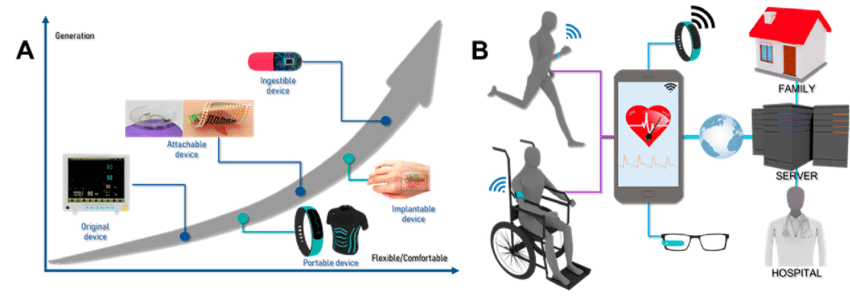
\includegraphics[scale=0.5]{images/wearable.png}
\caption{Σχηματική απεικόνιση των διάφορων εργαλείων της ένδυτης τεχνολογίας}.
\label{wearable}
\end{figure}

\subsubsection{``Έξυπνα'' κινητά και ρολόγια}
Τα ``έξυπνα'' κινητά (\en{smartphones}) είναι εξοπλισμένα με διάφορους αισθητήρες, όπως επιταχυνσιόμετρο, γυροσκόπιο, αισθητήρες εγγύτητας, \en{GPS}, \en{Bluetooth}, φωτογραφική μηχανή, μικρόφωνο και αισθητήρες περιβαλλοντικών συνθηκών, οι οποίοι μπορούν να αξιοποιηθούν για παρακολούθηση δραστηριότητας σε εσωτερικούς και εξωτερικούς χώρους \cite{Incel2013}.
Τα ``έξυπνα'' ρολόγια (\en{smartwatches}) έχουν επίσης χρησιμοποιηθεί για παρακολούθηση δραστηριότητας, καθώς είναι εξοπλισμένα με παρόμοιους αισθητήρες \cite{Chernbumroong2011}\cite{Sen2015}.
\par
Σε αντίθεση με τα \en{smartphones}, οι περιβραχιόνιες συσκευές είναι πιο αξιόπιστες στην αναγνώριση δραστηριοτήτων που περιλαμβάνουν κινήσεις χεριών, όπως η κατανάλωση φαγητού, ποτού ή το κάπνισμα \cite{Shoaib2016}.
Επίσης, παρέχουν συνεχή δεδομένα για την παρακολούθηση σε εσωτερικούς χώρους, καθώς μπορούν να φορεθούν άνετα 24 ώρες την ημέρα \cite{Bieber2013}\cite{Rawassizadeh2014}.
Τα \en{smartphones} έχουν καλύτερες επιδόσεις στην αναγνώριση των υπόλοιπων δραστηριοτήτων, διότι το μεγαλύτερο χρονικό διάστημα βρίσκονται κοντά στην λεκάνη, οπότε και είναι κατάλληλα για την αναγνώρισή δραστηριοτήτων, όπως η ποδηλασία ή το τρέξιμο \cite{Shoaib2016}\cite{Bieber2013}.
Πρόσφατες μελέτες προσπάθησαν να συνδυάσουν τα δεδομένα των αισθητήρων και από τις 2 συσκευές για προχωρημένη αναγνώριση δραστηριότητας \cite{Shoaib2016}\cite{Casilari2015}.
\par
Τα \en{smartwatches} και, συνολικά, οι περιβραχιόνιες συσκευές, λόγω της τοποθέτησης τους και της συνεχής επαφής τους με το δέρμα, είναι κατάλληλες για την παρακολούθηση φυσιολογικών δεικτών, όπως ο καρδιακός ρυθμός (μέσω του ηλεκτροκαρδιογραφήματος (\en{ECG}) ή του φωτοπληθυσμιογραφήματος (\en{PPG})), την θερμοκρασία του σώματος, την εφίδρωση (μέσω της ηλεκτροδερματικής δραστηριότητας \en{GSR}) και της μυϊκής δραστηριότητας (μέσω της ηλεκτρομυογραφήματος (\en{EMG})) \cite{Rawassizadeh2014}\cite{Klonovs2016}.
\par
Αρκετές έρευνες έχουν χρησιμοποιήσει \en{smartphones}, \en{smartwatches} και άλλες περιβραχιόνιες 
συσκευές στον τομέα των ΠΥΔ.
Συγκεκριμένα, έχουν χρησιμοποιηθεί διαθέσιμα στην αγορά \en{smartphones} και \en{smartwatches} για την αναγνώριση πτώσεων ηλικιωμένων ατόμων.
Η χρήση αυτών των συσκευών μείωσε τον αριθμό των λανθασμένων συναγερμών, ενώ ταυτόχρονα βελτίωσε την ικανότητα ανίχνευσης πραγματικών πτώσεων \cite{Casilari2015}.
Σε άλλες έρευνες, η αξιοποίηση των δεδομένων από τις συγκεκριμένες συσκευές απέτρεψε την αφυδάτωση ηλικιωμένων ατόμων μέσω της παρακολούθησης των κινήσεων των χεριών τους \cite{Lutze2015}.

\subsubsection{``Έξυπνα'' ρούχα και υφάσματα}
Τα ``έξυπνα'' ρούχα και υφάσματα προσφέρουν άλλο ένα εργαλείο για μη επεμβατική παρακολούθηση της υγείας και της δραστηριότητας των ατόμων.
Έχουν αναπτυχθεί αισθητήρες που μπορούν να ενσωματωθούν στα ρούχα, στο ύφασμα και στις ίνες του υφάσματος \cite{rashidi2012survey}.
Ένα παράδειγμα ενός ``έξυπνου'' ρούχου είναι το γιλέκο \en{MagIC}.
Το συγκεκριμένο γιλέκο διαθέτει πλεκτά ηλεκτρόδια για καταγραφή ηλεκτροκαρδιογραφήματος (\en{ECG}), έναν υφασμάτινο αισθητήρα πληθυσμιογραφήματος για την παρακολούθηση του αναπνευστικού ρυθμού και ένα επιταχυνσιόμετρο.
Χρησιμοποιήθηκε για την απομακρυσμένη παρακολούθηση καρδιοπαθών \cite{Rienzo2010}.
\par
Ένα παρόμοιο ρούχο είναι το \en{t-shirt} \en{Smart Vest}.\cite{Pandian2008}
Περιέχει αισθητήρες ενσωματωμένους στο ύφασμα, οι οποίοι συλλέγουν διάφορους φυσιολογικούς δείκτες, όπως το ηλεκτροκαρδιογράφημα (\en{ECG}), το φωτοπληθυσμιογράφημα για την μέτρηση της ροής και πιέσης του αίματος (\en{PPG}), την θερμοκρασία του σώματος, την εφίδρωση μέσω του \en{GSR}, αλλά και την τοποθεσία μέσω \en{GPS}.
Ταυτόχρονα, γίνονται έρευνες \cite{Chang2013} για να αναπτυχθούν υφασμάτινοι χωρητικοί αισθητήρες σε διάφορα σημεία του σώματος, με σκοπό την καταγραφή διάφορων φυσιολογικών δεικτών, όπως το ηλεκτροκαρδιογράφημα και ο ρυθμός αναπνοής, οι κινήσεις του καρπού και του χεριού, η κατανάλωση φαγητού και ποτού καθώς και πληροφορίες για το βάδισμα του ατόμου.
\par
Υπάρχουν και άλλες δημοφιλείς ένδυτες συσκευές, οι οποίες, συνήθως, επισυνάπτονται στα παπούτσια, στη ζώνη ή στα κοσμήματα του χρήστη \cite{Brodie2016}\cite{Achkar2016}\cite{Sardini2010}\cite{Sim2011}.
\subsubsection{Επιδερμικά ηλεκτρονικά συστήματα}
Ένα ακόμη αισθητηριακό εργαλείο για την καταγραφή της υγείας είναι αισθητήρες ενσωματωμένοι σε επιφάνειες, οι οποίες είναι συνημμένες στο δέρμα. 
Ωστόσο, η συγκεκριμένη λύση έχει περιορισμένη περιθώρια αξιοποίησης στην καθημερινή ζωή, καθώς δεν είναι εύχρηστη και οι αισθητήρες μπορούν εύκολα να αποσπαστούν από το δέρμα \cite{Yeo2013}.
Πρόσφατα, αναπτύχθηκαν εύκαμπτες και λεπτές μεμβράνες, οι οποίες ονομάζονται επιδερμικά ηλεκτρονικά συστήματα.
Οι ιδιότητες τους επιτρέπουν μια πιο σταθερή και στενή διεπαφή της μεμβράνης με το δέρμα, επιτρέποντας την συνεχή και σταθερή καταγραφή φυσιολογικών μετρήσεων \cite{Imani2016}.
Αν και τα περισσότερα παρόμοια συστήματα συλλέγουν φυσικές ή ηλεκτροφυσιολογικές παραμέτρους, όπως το ηλεκτροκαρδιογράφημα ή η θερμοκρασία του δέρματος \cite{Bian2014}\cite{Webb2013}\cite{Yeo2013}, υπάρχουν ορισμένα τα οποία συλλέγουν και βιοχημικές παραμέτρους, όπως η συγκέντρωση γαλακτικού οξέος στον ιδρώτα \cite{Imani2016}.
\subsubsection{Ενδοσωματικά συστήματα}
Μια πιο επεμβατική λύση για την παρακολούθηση της υγείας ενός χρήστη είναι τα συστήματα που εισέρχονται στο σώμα του.
Παραδείγματα τέτοιων λύσεων είναι αισθητήρες γλυκόζης, οι οποίοι εισέρχονται υποδόρια για την ανίχνευση υπογλυκαιμίας στο αίμα \cite{Juhl2010}.
και κάψουλες, οι οποίες χορηγούνται από το στόμα, και καταγράφουν την θερμοκρασία, την πίεση, εικόνες και το \en{pH} στο εσωτερικό του σώματος \cite{McCaffrey2008}.
\subsection{Υποβοηθητική ρομποτική}
Η υποβοηθητική ρομποτική στα ΠΥΔ χωρίζεται στις εξής 3 ευρείς κατηγορίες, τα ρομπότ ανάρρωσης και παροχής φροντίδας, τα κοινωνικά ρομπότ παροχής υπηρεσιών και τα ρομπότ συντροφιάς, όπως φαίνεται και στο Σχήμα \ref{robot_start} \cite{Broekens2009}\cite{Robinson2014}.
\begin{figure}[h!]
\centering
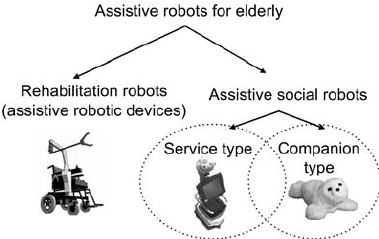
\includegraphics[scale=0.6]{images/robotics_start.png}
\caption{Σχηματική απεικόνιση των κατηγοριών της υποβοηθητικής ρομποτικής}.
\label{robot_start}
\end{figure}
Η πρώτη κατηγορία περιγράφεται ως ``συσκευές οι οποίες βοηθάνε φυσικά τον χρήστη χωρίς να έχουν κύριο σκοπό την επικοινωνία ή να μπορούν να θεωρηθούν κοινωνικές οντότητες'' \cite{Robinson2014}.
Τα ρομπότ ανάρρωσης βοηθούν στην φυσική εξάσκηση, συνεισφέρουν στην διαχείριση μειωμένων φυσικών
ικανοτήτων και βοηθούν τους ηλικιωμένους στις καθημερινές δραστηριότητες τους.
Παραδείγματα που ανήκουν σε αυτήν την κατηγορία είναι ρομπότ υποβοήθησης κίνησης \cite{Spenko2006}, εξωσκελετοί \cite{OSullivan2015} και ρομπότ που βοηθούν με την φυσική εξάσκηση και αποκατάσταση \cite{Johnson2006}.
\par
Η δεύτερη κατηγορία είναι τα κοινωνικά ρομπότ παροχής υπηρεσιών.
Ο σκοπός τους είναι να βοηθούν τους ηλικιωμένους στις διάφορες δραστηριότητες της καθημερινότητας, να βοηθούν στις μετακινήσεις τους και να παρακολουθούν την υγεία και ασφάλεια τους.
Τα συγκεκριμένα ρομπότ χαρακτηρίζονται ως κοινωνικά διότι μπορούν να αλληλεπιδράσουν άμεσα με τους ηλικιωμένους \cite{Robinson2014}.
Το ρομπότ \en{Pearl} είναι ένα ανθρωποειδές κοινωνικό ρομπότ παροχής υπηρεσιών, το οποίο έχει ύψος 1 μέτρο, και αλληλεπιδρά με τον χρήστη μέσω ομιλίας, οθονών, εκφράσεις του προσώπου και φυσική κίνηση \cite{Pineau2003}\cite{Pollack2002}.
Σχεδιάστηκε για να βοηθά ηλικιωμένους, μέσω της υπενθύμισης και της οργάνωσης διάφορων καθημερινών εργασιών και δραστηριοτήτων, όπως τα γεύματα, η φαρμακευτική αγωγή και η πλοήγηση στο περιβάλλον τους.
\par
Το ρομπότ \en{Care-o-bot} ανήκει στην ίδια κατηγορία \cite{Hans2002}\cite{Kittman2015}\cite{Reiser2013}.
Η τελευταία εκδοχή του είναι ανθρωπόμορφη και έχει ύψος 1.5 μέτρο.
Σε σχέση με τις προηγούμενες εκδοχές του, έχει δοθεί προσοχή στα μέσα αλληλεπίδρασης και στην φυσικότητα του σώματος του, για την βελτίωση της κοινωνικότητας του.
Ο χρήστης μπορεί να αλληλεπιδράσει μαζί του μέσω χειρονομιών, ομιλίας, οθόνης αφής και εφαρμογής σε κινητό.
Το \en{Care-o-bot} μπορεί να αντιδράσει με εκφράσεις του προσώπου, κινήσεις των χεριών και του σώματος καθώς και με τα ενσωματωμένα ηχεία του.
Με τα εύκαμπτα χέρια του μπορεί να μεταφέρει και να χειριστεί αντικείμενα \cite{Kittman2015}.
Άλλα παραδείγματα ρομπότ παροχής υπηρεσιών είναι το \en{RIBA} \cite{Mukai2010} και το \en{Kompa}{\"i} \cite{Kompai2017}.
\par
Η τρίτη κατηγορία είναι τα ρομπότ συντροφιάς.
Κυρία λειτουργία τους είναι η ενίσχυση της συναισθηματικής ευμάρειας και η μείωση της μοναξιάς, παρέχοντας συντροφιά και διευκολύνοντας τις κοινωνικές αλληλεπιδράσεις \cite{Broekens2009}.
Ένα παράδειγμα ρομπότ συντροφιάς είναι ο \en{Paro}, μια ρομποτική φώκια καλυμμένη με μαλακή γούνα.
O \en{Paro} αντιδρά στην ομιλία, στο να τον χαϊδεύουν και να τον κρατάνε, κουνώντας το κεφάλι και τα πτερύγια του, ανοιγοκλείνοντας τα μάτια του και μιμούμενος την φωνή μιας νεαρής φώκιας.
Σκοπός του είναι να προκαλέσει αντίστοιχα συναισθήματα με ένα πραγματικό κατοικίδιο, ώστε να μειωθεί το άγχος και η ανησυχία, προσφέροντας ψυχολογική παρηγοριά και τονώνοντας τις κοινωνικές επαφές \cite{Wada2005}.
\par
Ένα ακόμα ρομπότ συντροφιάς είναι ο \en{AIBO}, ένας κινητός ρομποτικός σκύλος με ενσωματωμένους αισθητήρες και ένα σκληρό πλαστικό εξωτερικό.
Ο \en{AIBO} μπορεί να κουνήσει το κεφάλι, την ουρά και τα πόδια του.
Έχει δοκιμαστεί σε περιβάλλοντα με ηλικιωμένους και έρευνες έδειξαν πως μειώνει το άγχος και την μοναξιά και ενισχύει την κοινωνική συμπεριφορά \cite{Kanamori2002}\cite{Tamura2004}.
Ο \en{Zora} είναι ένα ανθρωποειδές ρομπότ συντροφιάς, το οποίο στοχεύει να ενεργοποιήσει και να αλληλεπιδράσει με τους ηλικιωμένους, τραγουδώντας, χορεύοντας ή ενθαρρύνοντας φυσική εξάσκηση \cite{Helianthe2017}\cite{Melkas2016}\cite{Parviainen2016}.
\par
Τα τελευταία χρόνια, ο διαχωρισμός μεταξύ των 3 κατηγοριών γίνεται ολοένα και πιο ασαφής, καθώς οι κατασκευαστές ρομπότ υπηρεσίας περιλαμβάνουν περισσότερα κοινωνικά μέσα και μέσα αλληλεπίδρασης, για να αυξήσουν την αποδοχή των χρηστών.
Επομένως, είναι πιθανό τα μελλοντικά ρομπότ να παρέχουν και αυξημένη λειτουργική υποστήριξη αλλά και κοινωνική συντροφιά.
\begin{figure}[h!]
\centering
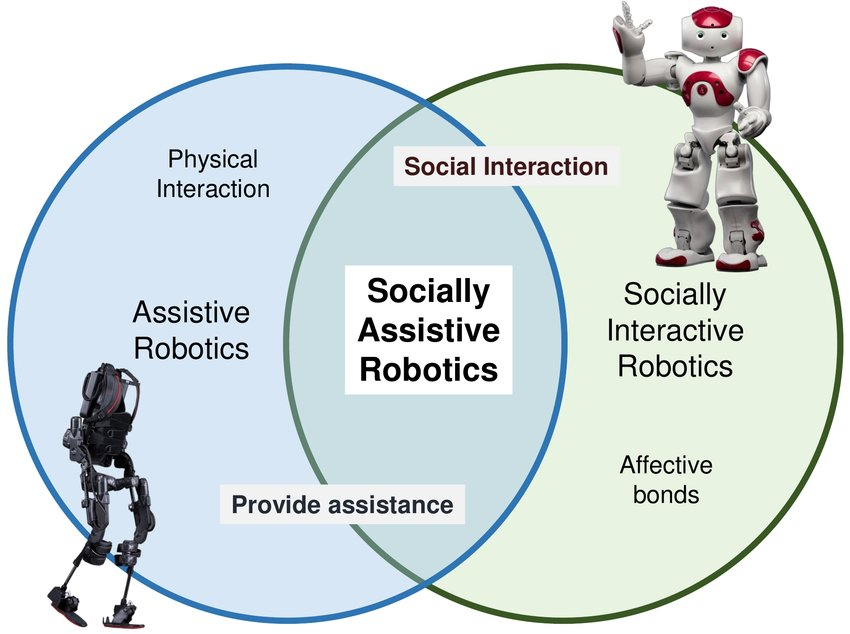
\includegraphics[scale=1]{images/robotics_end.jpg}
\caption{Σχηματική απεικόνιση των σκοπών της υποβοηθητικής ρομποτικής}.
\label{robot_end}
\end{figure}
\subsection{Αλγόριθμοι και υπολογιστικές τεχνικές}
Ο μεγάλος όγκος και ποικιλία των δεδομένων που συλλέγονται από τις διάφορες εφαρμογές των ΠΥΔ απαιτούν ειδικούς αλγορίθμους και υπολογιστικές τεχνικές για την κατανόηση και διαχείριση τους.
Παρακάτω θα παρουσιάσουμε μια περίληψη των πιο συχνών τεχνικών που χρησιμοποιούνται στις εφαρμογές των ΠΥΔ.

\subsubsection{Αναγνώριση δραστηριότητας}
Τα ΠΥΔ χρειάζονται να αναγνωρίσουν τι κάνουν οι χρήστες τους, βασισμένα σε μια ποικιλία δεδομένων, για να παρέχουν προληπτική βοήθεια.
Σημαντικές δραστηρίοτητες περιλαμβάνουν τον ύπνο, το περπάτημα, την εξάσκηση, την κατανάλωση φαγητού και ποτού και την λήψη της φαρμακευτικής αγωγής.
Η προσέγγιση για την αναγνώριση δραστηριότητας εξαρτάται από τους υποκείμενους αισθητήρες, τον αλγόριθμο μηχανικής μάθησης που μοντελοποιεί την δραστηριότητα και την πολυπλοκότητα της δραστηριότητας προς μάθηση.
\subsubsection{Αναγνώριση συμπεριφορικών μοτίβων}
Μια σχετική προσέγγιση είναι η αναγνώριση επαναλαμβανόμενων μοτίβων στα συγκεντρωμένα δεδομένα δραστηριότητας, μέσω τεχνικών μάθησης χωρίς επιτήρηση.
Τα μοτίβα αυτά συνεισφέρουν στην κατανόηση και ερμηνεία των δεδομένων που συλλέγονται από τους αισθητήρες και μπορούν να χρησιμοποιηθούν για την κατασκευή νέων μοντέλων για την αναγνώριση των μοτίβων αυτών στο μέλλον.
\subsubsection{Αναγνώριση ανωμαλιών}
Η αναγνώριση ανωμαλιών αναφέρεται στον εντοπισμό μοτίβων στα συγκεντρωμένα δεδομένα, τα οποία αποκλίνουν από την αναμενόμενη συμπεριφορά.
Αυτό είναι κομβικό για τα ΠΥΔ, για να μπορέσει να αναγνωρίσει αλλαγές στην καθημερινή ρουτίνα, μη συμμόρφωση με την φαρμακευτική αγωγή, πτώσεις ή άλλες επείγοντες καταστάσεις.
Η αναγνώριση ανωμαλιών είναι πιο ακριβής με συμπεριφορές, οι οποίες πραγματοποιούνται σε τακτική βάση.
\subsubsection{Μοντελοποίηση πλαισίου}
Τα συστήματα ΠΥΔ πρέπει να προσαρμόζονται σε δυναμικές πληροφορίες πλαισίου, σχετικά με το φυσικό περιβάλλον, τον χρήστη και το υπολογιστικό υπόβαθρο \cite{Bettini2010}.
Επομένως, τα συστήματα πρέπει να μπορούν να αναπαραστήσουν την συναφή πληροφορία, όπως η χωρική πληροφορία του περιβάλλοντος, το ιατρικό ιστορικό, το προφίλ και τις προτιμήσεις του χρήστη, την πληροφορία για τους υπάρχοντες αισθητήρες.
\subsubsection{Σχεδιασμός και οργάνωση}
Ο αυτοματοποιήμενος σχεδιασμός και οργάνωση μπορούν να έχουν μεγάλη αξία σε διάφορες ΠΥΔ εφαρμογές.
Παραδείγματα περιλαμβάνουν την υπενθύμιση των απαραίτητων δραστηριοτήτων σε άτομα με πνευματικές βλάβες και την αυτοματοποίηση της καθημερινής ρουτίνας ατόμων με φυσικά προβλήματα.
\subsubsection{Αναγνώριση ταυτότητας και τοποθεσίας}
Η ανάγκη για παρακολούθηση, ανίχνευση και παροχή προληπτικής και φυσικής βοήθειας στους χρήστες, εξυπηρετείται στα ΠΥΔ από συστήματα ταυτοποίησης και εντοπισμού των ηλικιωμένων ειδικά σε κατοικίες με πολλούς κατοίκους.

\section{Προκλήσεις}
Υπάρχουν αρκετές προκλήσεις στον τομέα των ΠΥΔ που δεν έχουν λυθεί ακόμα, παρά τις υποσχόμενες τεχνικές εξελίξεις.
\subsection{Τεχνική υλοποίηση}
Τα έξυπνα σπίτια και οι ένδυτες συσκευές συλλέγουν έναν πολύ μεγάλο όγκο δεδομένων.
Αυτά είναι η βάση της προσωποποιημένης, προληπτικής και περιβάλλουσας βοήθειας, ωστόσο συνεπάγονται σοβαρά ζητήματα ασφάλειας και ιδιωτικότητας.
Απαιτείται η χρήση πρωτοκόλλων ασφαλείας και η χρήση ειδικών τεχνικών προστασίας δεδομένων.
Αυτό είναι ιδιαίτερα σημαντικό για ευαίσθητα δεδομένα, όπως ιατρικά δεδομένα ή οπτικό υλικό.
Ο συνδυασμός των διάφορων διασυνδεδεμένων αισθητήρων και συσκευών περαιτέρω δυσχεραίνει την υλοποίηση ασφαλούς ανάλυσης και αποθήκευσης δεδομένων \cite{Acampora2013}\cite{Ghayvat2015}\cite{rashidi2012survey}.
Η διαλειτουργικότητα και η τυποποίηση των αισθητήρων και συσκευών, προκειμένου να μπορούν να επικοινωνήσουν μεταξύ τους, είναι ένα επιπλέον πρόβλημα το οποίο προσπαθούν να λύσουν οι ερευνητές \cite{Memon2014}\cite{Queiros2013}.
Επίσης, ένα συνολικό πρόβλημα που αντιμετωπίζουν τα ΠΥΔ είναι ο σχεδιασμός απλών και διαισθητικών διεπαφών, ώστε να διευκολυνθεί η φυσική αλληλεπίδραση με τα ηλικιωμένα άτομα \cite{Queiros2013}\cite{Sun2009}.
\par
Ένα ακόμα πρόβλημα των συστημάτων ΠΥΔ είναι η αξιοπιστία.
Η αξιόπιστη αναγνώριση της δραστηριότητας και της συμπεριφοράς του χρήστη σε ένα μη ελεγχόμενο οικιακό περιβάλλον είναι ένα απαιτητικό πρόβλημα.
Πολλές έρευνες αναφέρουν προβλήματα αξιοπιστίας, όπως λάθος συναγερμοί, χαμηλή ακρίβεια πρόβλεψης ή αδυναμία διαχείρισης πολλαπλών χρηστών, παρά την συνεχή εξέλιξη των αλγορίθμων και των αισθητήρων.
Τα ζητήματα αξιοπιστίας δεν οδηγούν μόνο σε δυσφορία και μειωμένη εμπιστοσύνη μεταξύ των χρηστών, αλλά μπορούν να έχουν σοβαρές επιπτώσεις στην υγεία και την ευμάρεια τους.
Επομένως, η βελτίωση της αξιοπιστίας των ΠΥΔ παραμένει κομβικό ζήτημα προς επίλυση \cite{Liu2016}\cite{rashidi2012survey}\cite{cardinaux}.
\par
Στην περίπτωση των ένδυτων λύσεων, υπάρχει η επιπλέον πρόκληση να σχεδιαστεί μια άνετη, ελαφριά και ασφαλής συσκευή με καλή αισθητική, σχεδιασμό και χαμηλή ενεργειακή κατανάλωση, ώστε να μπορεί και θέλει ο χρήστης να την φοράει 24 ώρες την μέρα.
Ταυτόχρονα, οι προγραμματιστές και οι σχεδιαστές αυτών των συσκευών χρειάζεται να ενσωματώσουν σε αυτές, το απαραίτητο υλικό και λογισμικό για αξιόπιστη, ασφαλή και συνεχή συλλογή δεδομένων \cite{Ghayvat2015}.
\par
Αντίστοιχα, η μεγαλύτερη πρόκληση της υποβοηθητικής ρομποτικής είναι η διευκόλυνση της φυσικής αλληλεπίδρασης και κοινωνικής σύμπλεξης μεταξύ ρομπότ και ηλικιωμένων.
Οι ερευνητές συνεχίζουν να δουλεύουν προς μια αποδεκτή φυσική εμφάνιση, τον σχεδιασμό χειρονομιών, εκφράσεων προσώπου και σωματικών κινήσεων που να προσεγγίζουν τις ανθρώπινες και την δημιουργία κοινωνικής νοημοσύνης και αυτόνομης συμπεριφοράς \cite{Robinson2014}\cite{Mataric2017}.
Επιπλέον, τα περισσότερα ρομπότ έχουν περιορισμένη λειτουργικότητα και δεν είναι σε θέση να βοηθήσουν σε πολλές και περίπλοκες δραστηριότητες της καθημερινότητας \cite{rashidi2012survey}.
Μια ακόμα ανησυχία για την υποβοηθητική ρομποτική είναι η εγγυημένη ασφαλής κίνηση και λειτουργία σε ένα οικιακό περιβάλλον \cite{Salem2015}.
\par
Παρά την εντυπωσιακή πρόοδο και τις πολλαπλές δυνατότητες που παρουσιάζονται, πρόσφατες συστηματικές έρευνες\cite{Liu2016}\cite{Memon2014} ανέδειξαν ότι η συνολική τεχνολογική ετοιμότητα των ΠΥΔ εφαρμογών παραμένει χαμηλή, με τις περισσότερες εφαρμογές να περιορίζονται σε πιλοτικό στάδιο και μόνο ένα μικρό μέρος να καταλήγει σε εμπορικά προϊόντα.
Ορισμένα από τα βασικά εμπόδια για την υλοποίηση και διάδοση των ΠΥΔ συστημάτων είναι η αβεβαιότητα του κόστους τους και η έλλειψη κανονισμών και ρυθμίσεων σχετικά με τον διαμοιρασμό και αποζημίωση του κόστους τους από τους αντίστοιχους ασφαλιστικούς φορείς \cite{rashidi2012survey}\cite{Reeder2013}\cite{Vimarlund2014}.
Ωστόσο, σύγχρονες έρευνες άρχισαν να προσεγγίζουν τα παραπάνω προβλήματα, αναλύοντας την αποδοτικότητα των συστημάτων ΠΥΔ με όρους κόστους και εξερευνώντας τρόπους να συνδέσουν τα ΠΥΔ συστήματα με τα διάφορα συστήματα υγείας \cite{Manetti2017}.
\subsection{Αποδοχή από τους χρήστες}
Η πιο σημαντική συνθήκη για την διάδοση των ΠΥΔ είναι η αποδοχή των χρηστών.
Αρκετές συστηματικές ανασκοπήσεις αναδεικνύουν την αποδοχή αυτή ως ένα από τα μεγάλα εμπόδια για την υλοποίηση και διάδοση των ΠΥΔ συστημάτων σε πραγματικές συνθήκες \cite{Peek2014}\cite{rashidi2012survey}\cite{Robinson2014}.
Όντως, η φύση και ο σκοπός των ΠΥΔ έχουν σημαντικές επιπτώσεις στην αποδοχή από τους χρήστες.
Αυτές οι συσκευές καταλαμβάνουν ιδιωτικό χώρο είτε στο οικιακό περιβάλλον είτε ακόμα και πάνω στο σώμα των χρηστών, συλλέγουν και αποθηκεύουν προσωπικά και ιατρικά δεδομένα, επηρεάζουν την συμπεριφορά και τις συνήθειες, ωθούν τους χρήστες τους να κοινωνικοποιηθούν μέσω ή με μια μηχανή και αναλαμβάνουν εργασίες οι οποίες προορίζονται για άνθρωπο, είτε τον ίδιο τον χρήστη ή κάποιο πάροχο φροντίδας.
\par
Η αποδοχή των χρηστών, λοιπόν, απασχολεί όλο και περισσότερες έρευνες \cite{Liu2016}.
Ωστόσο, ο τομέας παραμένει κινούμενος με γνώμονα την τεχνολογία και όχι τον χρήστη, καθώς οι ερευνητές και σχεδιαστές ΠΥΔ εφαρμογών δεν έχουν σαν προτεραιότητα την κάλυψη των αναγκών των χρηστών \cite{Queiros2013}.
Αυτό οδηγεί σε στερεοτυπικές συμπεριφορές, υπεραπλούστευση και ανεπαρκής κατανόηση των αναγκών του χρήστη, τα οποία συνεπώς, οδηγούν σε κακό σχεδιασμό και υλοποίηση προϊόντων τα οποία τείνουν να απορρίπτονται από τους χρήστες \cite{Eisma2004}\cite{Ostlund2005}\cite{Peine2014}\cite{Vines2015}.
\par
Επομένως, οι ηλικιωμένοι και οι πάροχοι υγείας πρέπει να εμπλακούν στην διαδικασία σχεδιασμού και ανάπτυξης έτσι ώστε να αποφευχθεί ένα κενό μεταξύ των αναγκών των χρηστών και τις πεποιθήσεις των ερευνητών \cite{rashidi2012survey}\cite{Piau2013}\cite{Queiros2013}.
Επιπλέον, ο κλάδος οφείλει να αναπτύξει μια περιεκτική κατανόηση, βασισμένη στην θεωρία, τον παραγόντων αυτών που προωθούν ή αποθαρρύνουν την αποδοχή των ΠΥΔ.
Τα συμπεράσματα αυτά μπορούν να αξιοποιηθούν στις διαδικασίες σχεδιασμού και ανάπτυξης νέων προϊόντων, αυξάνοντας έτσι την πιθανότητα αποδοχής τους από τους μελλοντικούς τους χρήστες.
\subsection{Εφαρμογές μεγάλης κλίμακας και θεωρητικός διάλογος}
Οι περισσότερες έρευνες σχετικά με τα ΠΥΔ υποστηρίζουν ότι οι τεχνολογίες αυτές έχουν την δυνατότητα υποστήριξης μιας υγιούς και αυτόνομης γήρανσης για τους ηλικιωμένους, ωστόσο οι κλινικές ενδείξεις είναι λίγες και αδύναμες.
Η κλινική αποδεικτική βάση των ΠΥΔ παρουσιάζει μικτά αποτελέσματα. Ενώ οι \en{Demiris} και \en{Hensel} σε πρώιμη μελέτη δεν εντόπισαν σαφείς ενδείξεις για τη βελτίωση της υγείας ή την αποφυγή θεσμικής φροντίδας \cite{Demiris2008}, μεταγενέστερες αναλύσεις, όπως αυτή του \en{Liu}, βρήκαν υποσχόμενες ενδείξεις για συγκεκριμένες εφαρμογές, όπως η παρακολούθηση καθημερινών δραστηριοτήτων, η υποστήριξη σε γνωστικές παθήσεις, η ψυχική υγεία και η καρδιολογική φροντίδα \cite{Liu2016}.
Οι ερευνητές δεν βρήκαν κάποια μελέτη που να παρουσιάζει κλινικά στοιχεία για την πρόβλεψη αναπηρίας, την αποφυγή πτώσεων και την βελτίωση της ποιότητας ζωής των χρηστών.
Ο \en{Robinson} κατέληξε ότι η υποβοηθητική ρομποτική χρειάζεται περισσότερες δοκιμές σε πραγματικά οικιακά περιβάλλοντα, ώστε να αποδειχθεί η δυνατότητα προσαρμογής τους στην καθημερινότητα ηλικιωμένων ατόμων και, στη συνέχεια, αποτελεσματικής υποστήριξης τους \cite{Robinson2014}.
\par
Η δεδομένη μεθοδολογική προσέγγιση για να μετρήσουν την αποδοχή των χρηστών είναι ποιοτική και όχι ποσοτική, ενώ ο αριθμός των δειγμάτων συνήθως είναι μικρός.
Είναι απαραίτητη η διεξαγωγή μεγαλύτερης κλίμακας ερευνών για να κατανοηθεί η σχετική σημασία των παραγόντων που επηρεάζουν την αποδοχή των ΠΥΔ από τους χρήστες, η αναγνώριση των υποκείμενων σχέσεων μεταξύ τους και η εξαγωγή συμπερασμάτων για την επίδραση τους στην διαδικασία αποδοχής.
Άλλες έρευνες αναφέρουν την ανησυχία ότι ο τομέας των ΠΥΔ είναι πλούσιος σε δεδομένα και όχι σε θεωρία \cite{Blackman2016}.
Αυτή η έλλειψη θεωρητικού πλαισίου επιβεβαιώνεται από τον \en{Liu}, ο οποίος διαπίστωσε ότι οι περισσότερες μελέτες αποδοχής των ΠΥΔ στερούνται θεωρητικής θεμελίωσης για την εξήγηση των ευρημάτων τους \cite{Liu2016}.
Η ανάπτυξη ενός θεωρητικού διαλόγου θα βοηθούσε τους ερευνητές των ΠΥΔ να κατανοήσουν τους υποκείμενους κοινωνικούς, ψυχολογικούς και συμπεριφορικούς μηχανισμούς της διαδικασίας αποδοχής.
\par
Συνολικά, είναι σαφές πως υπάρχει έλλειψη αποδεδειγμένων μεθοδολογικών προσεγγίσεων, όπως τυχαία ελεγχόμενες δοκιμές, μακροχρόνιες μελέτες, ποσοτικές μελέτες μεγάλης κλίμακας και θεωρητικές προσεγγίσεις, για την κατανόηση της διάδοσης και της αποδοτικότητας των εφαρμογών ΠΥΔ \cite{Martin2008}\cite{Morris2013}\cite{Peek2014}.
%\chapter{Θεωρία Ασαφών Συνόλων και Λογική}
\label{chap3}
Σε αυτό το κεφάλαιο παρουσιάζονται οι βασικές έννοιες της θεωρίας ασαφών συνόλων και της ασαφούς λογικής.
Οι \en{Klir} και \en{Yuan} \cite{KlirYuan} παρέχουν πιο αναλυτικές περιγραφές των αρχών της, ενώ οι \en{Nguyen} και \en{Walker} \cite{Nguyen} αναφέρονται σε πρακτικές εφαρμογές της. 
Η ασαφής λογική διευρύνει την κλασική θεωρία συνόλων και βοηθά στην ανάλυση δεδομένων που προέρχονται από βιοϊατρικές εφαρμογές στο πλαίσιο του Διαδικτύου των Πραγμάτων (\en{IoT}).

\section{Εισαγωγή}

Η μαθηματική λογική άρχισε να διαμορφώνεται στα μέσα του 19ου αιώνα, με σημαντικές συμβολές από τους \en{Boole} και \en{De Morgan}. Η προσπάθεια θεμελίωσης των Μαθηματικών ενσωμάτωσε τη φιλοσοφική λογική σε τυπικούς κανόνες. Μέσα σε αυτό το πλαίσιο, αναδείχθηκε η θεωρία συνόλων ως βασικό εργαλείο. Ορίζει σύνολα ως συλλογές αντικειμένων και στηρίζεται σε μια δυαδική σχέση μεταξύ ενός στοιχείου και ενός συνόλου: ανήκει ή δεν ανήκει.

Σύμφωνα με την κλασική θεωρία συνόλων, κάθε στοιχείο ενός συνόλου αναφοράς \(\Omega\) είτε βρίσκεται στο \(A\) είτε όχι. Η χαρακτηριστική συνάρτηση \(\chi_A\) διαχωρίζει ξεκάθαρα τα στοιχεία που ανήκουν στο \(A\) (τιμή 1) από αυτά που δεν ανήκουν (τιμή 0). Αυτό λειτουργεί καλά σε περιπτώσεις που οι έννοιες είναι σαφώς ορισμένες. Στη βιοϊατρική πράξη, όμως, συναντούμε ασάφεια. Συχνά, ένα στοιχείο ταιριάζει σε μια κατηγορία, αλλά όχι με απόλυτη βεβαιότητα.

Η θεωρία ασαφών συνόλων επεκτείνει τη δυαδική προσέγγιση και επιτρέπει ένα εύρος τιμών μεταξύ 0 και 1. Ο \en{Zadeh} \cite{Zadeh1965} παρατήρησε ότι πολλά σύνολα δεν έχουν καθαρά όρια και εισήγαγε την έννοια της συνάρτησης συμμετοχής. Με αυτόν τον τρόπο, αποτυπώνεται ο βαθμός στον οποίο κάθε στοιχείο συμμετέχει σε ένα ασαφές σύνολο, αντί για ένα απλό ``ναι'' ή ``όχι''.

Στα επόμενα τμήματα θα δούμε πώς αυτές οι συναρτήσεις συμμετοχής και οι πράξεις (συμπλήρωμα, τομή, ένωση) ορίζουν ένα πλαίσιο για την ασαφή λογική. Θα εστιάσουμε σε τρόπους με τους οποίους αυτή η προσέγγιση μπορεί να στηρίξει την επεξεργασία δεδομένων σε \en{IoT} εφαρμογές, κυρίως σε βιοϊατρικά περιβάλλοντα, όπου η αβεβαιότητα είναι συχνή.
Στα επόμενα κεφάλαια θα φανεί πώς αυτή η θεωρία μπορεί να εφαρμοστεί σε σύνθετες αναλύσεις δεδομένων, όπως οι μετρικές ομοιότητας ή απόστασης σε βιοϊατρικά σήματα από IoT συσκευές.

\section{Θεωρία Ασαφών Συνόλων}
Βασιζόμενοι στη συζήτηση για τους περιορισμούς των κλασικών (αυστηρών) συνόλων, προχωρούμε στον τυπικό ορισμό και την ερμηνεία των ασαφών συνόλων. Η βασική αρχή είναι ότι πολλές πραγματικές καταστάσεις περιλαμβάνουν ασάφεια και αβεβαιότητα, που δεν μπορούν να αποδοθούν ικανοποιητικά με ένα δυαδικό σχήμα ``ανήκει/δεν ανήκει'' \cite{Zadeh1965,KlirYuan}. Εντός αυτού του πλαισίου, ο \en{Zadeh} προέτεινε μια γενίκευση της κλασικής θεωρίας συνόλων, εισάγοντας την έννοια του βαθμού συμμετοχής κάθε στοιχείου.

\begin{figure}[h!] 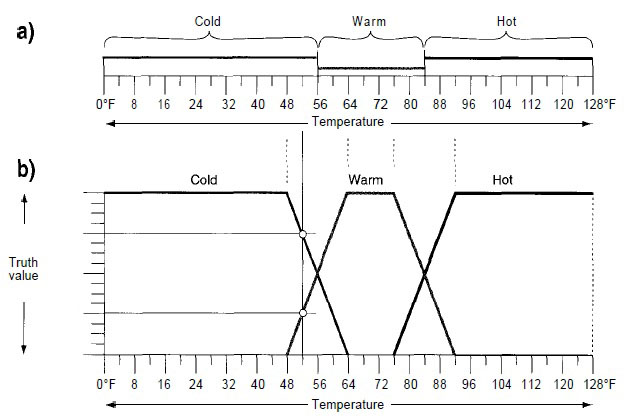
\includegraphics[scale=0.7]{images/fuzzy_logic1.jpg} \centering \caption{(\textlatin{a}) Παράδειγμα αυστηρού (\textlatin{crisp}) συνόλου, (\textlatin{b}) Παράδειγμα ασαφούς συνόλου.} \label{char_fun1} \end{figure}

\medskip

\begin{definition}
	\label{def:fuzzyset}
	\textbf{Ορισμός Ασαφούς Συνόλου.}\\
	Έστω \(\Omega\) ένα σύνολο αναφοράς. Ορίζουμε ένα \emph{ασαφές σύνολο} \(A \subseteq \Omega\) ως το διατεταγμένο ζεύγος
	\begin{equation}
	\label{eq:1}
	A = \{(x,\ \mu_{A}(x)) \mid x \in \Omega,\ \mu_{A}: \Omega \rightarrow [0,1]\},
	\end{equation}
	όπου \(\mu_{A}(x)\) είναι η \emph{συνάρτηση συμμετοχής} του \(x\) στο \(A\). Η τιμή \(\mu_{A}(x)\) μπορεί να λάβει οποιαδήποτε πραγματική τιμή στο διάστημα \([0,1]\), εκφράζοντας σε ποιον βαθμό το στοιχείο \(x\) ανήκει στο ασαφές σύνολο \(A\).
\end{definition}

Στο Σχήμα~\ref{char_fun1}\,(\textlatin{b}) παρουσιάζεται η γραφική απεικόνιση μιας τέτοιας συνάρτησης συμμετοχής, σε αντιδιαστολή με το αυστηρό (\(\{0,1\}\)) σχήμα του κλασικού συνόλου στο Σχήμα~\ref{char_fun1}\,(\textlatin{a}). 

\medskip
Σε περιπτώσεις όπου το ασαφές σύνολο \(A\) είναι \emph{διακριτό}, μπορούμε να το συμβολίσουμε ως:
\begin{equation}
\label{eq:2}
A = \sum_{i=1}^{n} \mu_{A}(x_{i})/x_{i},
\end{equation}
όπου το σύμβολο \(\sum\) υποδηλώνει την ``ένωση'' όλων των στοιχείων και \(\mu_{A}(x_{i})/x_{i}\) σημαίνει ότι το στοιχείο \(x_{i}\) ανήκει στο \(A\) με βαθμό συμμετοχής \(\mu_{A}(x_{i})\). Σημειώνεται ότι ο χαρακτήρας "/" δεν δηλώνει διαίρεση αλλά συμβατική σημείωση που απαντάται συχνά στη βιβλιογραφία \cite{DuboisPrade1980}.

\medskip
Αντίστοιχα, όταν το \(A\) είναι \emph{συνεχές}, γράφεται:
\begin{equation}
\label{eq:3}
\int_{x} \mu_{A}(x)/x,
\end{equation}
όπου το ολοκλήρωμα \(\int\) καταδεικνύει την ``ένωση'' σε έναν συνεχόμενο χώρο αναφοράς \(\Omega\).

\begin{definition}
	\label{def:normal}
	\textbf{Κανονικό Ασαφές Σύνολο.}\\
	Ένα ασαφές σύνολο \(A\) καλείται \emph{κανονικό} (\textlatin{normal}) εάν η συνάρτηση συμμετοχής του φτάνει το 1 για τουλάχιστον ένα στοιχείο:
	\begin{equation}
	\label{eq:4}
	\max_{x \in \Omega} \mu_{A}(x) = 1.
	\end{equation}
	Με άλλα λόγια, υπάρχει τουλάχιστον ένα \(x \in \Omega\) που ανήκει στο \(A\) με πλήρη βαθμό συμμετοχής.
\end{definition}

\begin{definition}
	\textbf{Πληθικότητα Ασαφούς Συνόλου (\en{Cardinality}).}\\
	Για ένα πεπερασμένο σύνολο αναφοράς \(\Omega\), ορίζουμε την \emph{πληθικότητα} του ασαφούς συνόλου \(A\) ως:
	\begin{equation}
	\label{eq:5}
	|A| = \sum_{x \in \Omega} \mu_{A}(x).
	\end{equation}
	Αντίστοιχα, η \emph{σχετική πληθικότητα} του \(A\) ως προς \(\Omega\) είναι:
	\begin{equation}
	\|A\| = \frac{|A|}{|\Omega|}.
	\end{equation}
	Οι έννοιες αυτές ποσοτικοποιούν το πόσο ``μεγάλο'' είναι το ασαφές σύνολο, λαμβάνοντας υπόψη τους μη-δυαδικούς βαθμούς συμμετοχής \cite{KlirYuan}.
\end{definition}

Στον Πίνακα~\ref{tab:part} συνοψίζονται μερικές από τις πιο διαδεδομένες μορφές συναρτήσεων συμμετοχής. Οι παραμετρικές εκφράσεις (π.χ. \(a, b, c, d, \sigma\)) καθορίζουν το σχήμα της συνάρτησης, καθιστώντας τη χρήσιμη για διαφορετικές εφαρμογές. Για παράδειγμα, η τριγωνική και η τραπεζοειδής μορφή προσφέρουν απλές, κομμάτι-γραμμικές προσεγγίσεις, ενώ η \textlatin{Gaussian} υποστηρίζει ομαλότερες μεταβάσεις \cite{Ross2010}.

\begin{table}[h!]
    \centering
    \begin{tabularx}{\textwidth}{>{\hsize=.4\hsize}X X >{\hsize=.5\hsize}X}
        \textbf{Συνάρτηση} & \textbf{Τύπος} & \textbf{Γραφική απεικόνιση} \\
        \hline
         \textbf{Τριγωνική} 
         & \(\displaystyle \mu_{A}(x) = \max\Bigl[\min\Bigl\{\tfrac{x-a}{b-a}, \tfrac{c-x}{c-b}\Bigr\}, 0\Bigr]\)
         & \begin{center}
             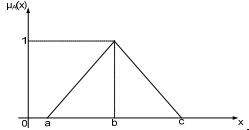
\includegraphics[scale=0.7]{images/trig.jpg}
           \end{center} \\
         \textbf{Τραπεζοειδής}
         & \(\displaystyle \mu_{A}(x) = \max\Bigl[\min\Bigl\{\tfrac{x-a}{b-a}, 1, \tfrac{d-x}{d-c}\Bigr\}, 0\Bigr]\)
         & \begin{center}
             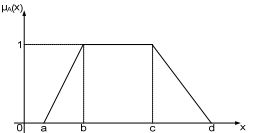
\includegraphics[scale=0.7]{images/trapez.jpg}
           \end{center}\\
         \textbf{\textlatin{Gaussian}}
         & \(\displaystyle \mu_{A}(x) = e^{-\bigl(\tfrac{x-b}{\sigma}\bigr)^2}\)
         & \begin{center}
             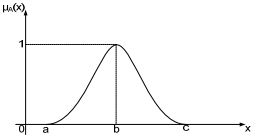
\includegraphics[scale=0.7]{images/gauss.jpg}
           \end{center}\\
         \textbf{Καμπανοειδής}
         & \(\displaystyle \mu_{A}(x) = \Bigl(1 + \Bigl|\tfrac{x-c}{a}\Bigr|^{2b}\Bigr)^{-1}\)
         & \begin{center}
             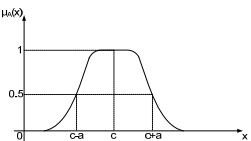
\includegraphics[scale=0.7]{images/bell.jpg}
           \end{center}\\
         \textbf{Σιγμοειδής}
         & \(\displaystyle \mu_{A}(x) = \bigl(1 + e^{-\,a\,(x-c)}\bigr)^{-1}\)
         & \begin{center}
             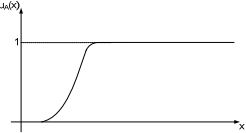
\includegraphics[scale=0.7]{images/sigm.jpg}
           \end{center}\\
    \end{tabularx}
    \caption{Παραδείγματα κοινών συναρτήσεων συμμετοχής (βάσει \cite{KlirYuan1995,Ross2010}).}
    \label{tab:part}
\end{table}

\medskip
Οι διαφορετικές μορφές παρουσιάζουν πλεονεκτήματα ανάλογα με την εκάστοτε εφαρμογή· για παράδειγμα, η τριγωνική συναρτήση συχνά χρησιμοποιείται για συστήματα με απλούς υπολογισμούς, ενώ η \textlatin{Gaussian} είναι κατάλληλη όταν οι μεταβάσεις πρέπει να είναι πιο ομαλές \cite{Zadeh1965,Ross2010}.

\medskip
Σε επόμενη ενότητα, θα ασχοληθούμε με τις πράξεις επί των ασαφών συνόλων (τομή, ένωση, συμπλήρωμα) και θα αναδείξουμε πώς αυτές γενικεύουν τις αντίστοιχες κλασικές πράξεις, καλύπτοντας μεγαλύτερη γκάμα εφαρμογών που χαρακτηρίζονται από αβεβαιότητα ή \emph{μερική αλήθεια}. Έτσι, το θεωρητικό υπόβαθρο που περιγράφεται σε αυτό το κεφάλαιο αποτελεί τη βάση για την περαιτέρω ανάπτυξη ασαφών συστημάτων και μεθόδων συμπερασμού.

\section{Τελεστές Ασαφούς Συνολοθεωρίας}

Στην κλασική θεωρία συνόλων, οι πράξεις της τομής, της ένωσης και του συμπληρώματος καθορίζουν πώς τα σύνολα αλληλεπιδρούν. Στο πλαίσιο των ασαφών συνόλων, οι ίδιες πράξεις γενικεύονται, ώστε να διαχειρίζονται βαθμούς συμμετοχής \cite{Zadeh1965,KlirYuan}. Η επιλογή της κατάλληλης ασαφούς πράξης εξαρτάται από τις απαιτήσεις της εφαρμογής.  

\subsection{Βασικές Σχέσεις: Κενό, Υποσύνολο, Ισότητα}

Όπως στην κλασική θεωρία, ορίζουμε το κενό ασαφές σύνολο \(\emptyset\) όταν η συνάρτηση συμμετοχής είναι μηδενική παντού:
\begin{equation}
    A = \emptyset \;\;\; \Longleftrightarrow \;\;\; \mu_{A}(x) = 0, \;\; \forall x\in \Omega.
\end{equation}
Δύο ασαφή σύνολα \(A\) και \(B\) θεωρούνται ίσα αν έχουν την ίδια συνάρτηση συμμετοχής:
\begin{equation}
    A = B \;\;\; \Longleftrightarrow \;\;\; \mu_{A}(x) = \mu_{B}(x), \;\; \forall x \in \Omega.
\end{equation}
Ο ορισμός του υποσυνόλου διαφοροποιείται από την κλασική περίπτωση ως εξής:
\begin{equation}
    A \subseteq B \;\;\; \Longleftrightarrow \;\;\; \mu_{A}(x) \leq \mu_{B}(x), \;\; \forall x \in \Omega,
\end{equation}
υποδηλώνοντας ότι ένα ασαφές σύνολο \(A\) είναι υποσύνολο ενός ασαφούς συνόλου \(B\) εάν η συνάρτηση συμμετοχής του είναι μικρότερη ή ίση αυτής του \(B\), για κάθε αντικείμενο του συνόλου αναφοράς \(\Omega\). Αυτό συχνά επιτρέπει στο \(A\) και το \(B\) να έχουν το ίδιο πλήθος στοιχείων, αλλά με διαφορετικούς βαθμούς συμμετοχής \cite{DuboisPrade1980}.

\subsection{Ασαφές Συμπλήρωμα}

Το συμπλήρωμα ενός ασαφούς συνόλου \(A\) ορίζεται από μια συνάρτηση 
\(
C : [0,1] \rightarrow [0,1],
\)
η οποία, για κάθε \(x \in \Omega\), αντιστοιχίζει τον βαθμό συμμετοχής \(\mu_A(x)\) στο βαθμό συμμετοχής του \(x\) στο συμπληρωματικό σύνολο \(\bar{A}\) \cite{Ross2010}. 
Οι συναρτήσεις αυτές οφείλουν να ικανοποιούν τα εξής αξιώματα:
\begin{enumerate}[label=(\textbf{\en{C}\arabic*)}, align=left, leftmargin=1em]
    \item Οριακές συνθήκες --- \(C(0) = 1\) και \(C(1) = 0\), δηλαδή ο ασαφής τελεστής \(C\) συμπεριφέρεται όπως το τυπικό συμπλήρωμα στις οριακές συνθήκες.
    \item Μονοτονία --- \(a<b \implies C(a) \geq C(b),\ \ \forall a,b \in [0,1]\), δηλαδή ο τελεστής \(C\) πρέπει να είναι μια φθίνουσα συνάρτηση.
\end{enumerate}
\par
Πέρα από τα παραπάνω, συνήθως λαμβάνονται υπόψη και άλλα 2 αξιώματα, τα οποία περιορίζουν την κλάση των συναρτήσεων που ικανοποιούν τα παραπάνω.
\begin{enumerate}[label=(\textbf{\en{C}\arabic*)}, align=left, leftmargin=1em]
    \setcounter{enumi}{2}
    \item Συνέχεια --- Ο τελεστής \(C\) να είναι συνεχής.
    \item Ενέλιξη --- \(C(C(a)) =a\)
\end{enumerate}

Οι πιο διαδεδομένες συναρτήσεις συμπληρώματος φαίνονται στον Πίνακα~\ref{tab:supp}, με κεντρικότερη:
\begin{equation}
    C(x) = 1 - x.
\end{equation}

\begin{table}[h!]
    \centering
    \begin{tabularx}{\textwidth}{X X}
        \textbf{Συνάρτηση} & \textbf{Τύπος}\\
        \hline
        \rule{0pt}{5ex}\textbf{Πρότυπο}
        & \(\displaystyle C(x) = 1 - x\) \\
        \rule{0pt}{5ex}\textbf{Κατώφλι}
        & \(\displaystyle C(x) = \begin{cases}
              1, & x \leq \tau \\
              0, & \text{αλλιώς}
           \end{cases}, \quad \tau \in [0,1]\)\\
        \rule{0pt}{5ex}\textbf{Συνημιτονοειδές}
        & \(\displaystyle C(x) = \frac{1 + \cos(\pi x)}{2}\)\\
        \textbf{\textlatin{Sugeno}}
        & \(\displaystyle C(x) = \frac{1 - x}{1 + \lambda x}, \quad \lambda > -1\)\\
        \textbf{\textlatin{Yagar}}
        & \(\displaystyle C(x) = (1 - x^w)^{\tfrac{1}{w}}, \quad w>0\)
    \end{tabularx}
    \caption{Συναρτήσεις ασαφούς συμπληρώματος \cite{Zadeh1965,DuboisPrade1980}.}
    \label{tab:supp}
\end{table}

\subsection{Ασαφής Τομή (\en{t-norm})}

Η ασαφής τομή δύο ασαφών συνόλων \(A\) και \(B\) δίνεται από έναν \textit{δυαδικό τελεστή} 
\[
T : [0,1]\times[0,1] \to [0,1],
\]
γνωστό και ως \textit{\en{triangular norm}} (\textit{\en{t-norm}}). 
Έχει καθιερωθεί πως οι συναρτήσεις, οι οποίες σχετίζονται με την πράξη της τομής, χρειάζεται να ικανοποιούν τα εξής αξιώματα, για \(a,b,c,d \in [0,1]\):
\begin{enumerate}[label=(\textbf{\en{T}\arabic*)}, align=left, leftmargin=1em]
    \item Οριακές συνθήκες --- \(T(1,a) = a\)
    \item Μονοτονία --- \(a \leq c\ \wedge\ b \leq d  \implies T(a,b) \leq T(c,d)\)
    \item Αντιμεταθετική ιδιότητα --- \( T(a,b) = T(b,a) \)
    \item Προσεταιριστική ιδιότητα --- \( T(a,T(b,c)) =T(T(a,b),c) \)
\end{enumerate}
Η απλούστερη και πιο διαδεδομένη συνάρτηση τομής είναι:
\begin{equation}
    T(a,b) = \min(a,b),
\end{equation}
όμως υπάρχουν εναλλακτικές, όπως το \(\textit{αλγεβρικό γινόμενο}\) ή η \(\textit{φραγμένη διαφορά}\) (Πίνακας~\ref{tab:inter}).
Στις πρακτικές εφαρμογές του IoT, η επιλογή της συνάρτησης \en{t-norm} είναι καθοριστική για τη συνδυαστική αξιολόγηση πολλών μετρικών από διαφορετικούς αισθητήρες (π.χ. συνδυάζοντας “ήπια” κατώφλια πίεσης και θερμοκρασίας).

\begin{table}[h!]
    \centering
    \begin{tabularx}{\textwidth}{X X}
        \textbf{Συνάρτηση} & \textbf{Τύπος}\\
        \hline
        \rule{0pt}{5ex}\textbf{Πρότυπο}
        & \(\displaystyle T(a,b) = \min(a,b)\)\\
        \rule{0pt}{5ex}\textbf{Δραστικό γινόμενο}
        & \(\displaystyle T(a,b) = \begin{cases}
              a, & b=1\\
              b, & a=1\\
              0, & \text{αλλιώς}
        \end{cases}\)\\
        \textbf{Αλγεβρικό γινόμενο}
        & \(\displaystyle T(a,b) = a\cdot b\)\\
        \textbf{Φραγμένη διαφορά}
        & \(\displaystyle T(a,b) = \max(0,a + b - 1)\)
    \end{tabularx}
    \caption{Παραδείγματα \en{t-norm} (ασαφούς τομής)}
    \label{tab:inter}
\end{table}

\subsection{Ασαφής Ένωση (\en{t-conorm})}

Ανάλογα, η ασαφής ένωση ορίζεται από έναν \textit{\en{t-conorm}} (\textit{\en{triangular conorm}}), 
\[
S : [0,1]\times[0,1] \to [0,1],
\]
που πληρεί αντίστοιχα αξιώματα (οριακές συνθήκες, μονοτονία, αντιμεταθετικότητα, προσεταιριστικότητα) \cite{DuboisPrade1980}. Ο τυπικός ορισμός είναι:
\begin{equation}
    S(a,b) = \max(a,b),
\end{equation}
αλλά και εδώ υπάρχουν διάφορες εναλλακτικές (Πίνακας~\ref{tab:un}). 
Συστήματα ελέγχου ή συστήματα υποστήριξης απόφασης συχνά χρησιμοποιούν ελαστικότερες \en{t-conorm} για να συνδυάσουν πολλαπλά κριτήρια με διαφορετικούς βαθμούς ικανοποίησης \cite{Zadeh1965,KlirYuan}. Για παράδειγμα, το αλγεβρικό άθροισμα επιτρέπει πιο ομαλή συνάθροιση των επιμέρους βαθμών συμμετοχής.

\begin{table}[h!]
    \centering
    \begin{tabularx}{\textwidth}{X X}
        \textbf{Συνάρτηση} & \textbf{Τύπος}\\
        \hline
        \rule{0pt}{5ex}\textbf{Πρότυπο}
        & \(\displaystyle S(a,b) = \max(a,b)\)\\
        \rule{0pt}{5ex}\textbf{Δραστικό άθροισμα}
        & \(\displaystyle S(a,b) = \begin{cases}
              a, & b=0\\
              b, & a=0\\
              1, & \text{αλλιώς}
        \end{cases}\)\\
        \textbf{Αλγεβρικό άθροισμα}
        & \(\displaystyle S(a,b) = a + b - ab\)\\
        \textbf{Φραγμένο άθροισμα}
        & \(\displaystyle S(a,b) = \min(1, a + b)\)
    \end{tabularx}
    \caption{Βασικοί τελεστές ασαφούς ένωσης (\en{t-conorm})}
    \label{tab:un}
\end{table}

\subsection{Ασαφής Συνεπαγωγή}

Η ασαφής συνεπαγωγή δίνεται από έναν \textit{δυαδικό τελεστή}
\[
J : [0,1]\times[0,1] \to [0,1],
\]
γνωστό και ως \textit{ασαφή συνεπαγωγή} (\textit{\en{fuzzy implication}}).
Έχει καθιερωθεί πως οι συναρτήσεις, οι οποίες σχετίζονται με την πράξη της συνεπαγωγής, χρειάζεται να ικανοποιούν τα εξής αξιώματα, για \(a,b,c,d \in [0,1]\):
\begin{enumerate}[label=(\textbf{\en{I}\arabic*)}, align=left, leftmargin=1em]
    \item Οριακές συνθήκες --- \(J(0,a) = 1\) και \(J(1,a) = a\)
    \item Μονοτονία στο δεύτερο όρισμα --- \(b \leq d \implies J(a,b) \leq J(a,d)\)
    \item Αντιμονοτονία στο πρώτο όρισμα --- \(a \leq c \implies J(c,b) \leq J(a,b)\)
\end{enumerate}

Η απλούστερη και πιο διαδεδομένη συνάρτηση συνεπαγωγής είναι:
\begin{equation}
    J(a,b) = \max(1-a,b),
\end{equation}
όμως υπάρχουν εναλλακτικές, όπως η \textit{συνεπαγωγή \en{Lukasiewicz}} ή η \textit{συνεπαγωγή \en{Mamdani}} (Πίνακας~\ref{tab:imply}) \cite{Zadeh1965,KlirYuan,Ross2010}.

\begin{table}[h!]
    \centering
    \begin{tabularx}{\textwidth}{X X}
       \textbf{Συνάρτηση} & \textbf{Τύπος}\\
       \hline
       \rule{0pt}{3ex} \textbf{\textlatin{Zadeh}}
       & \(a \rightarrow b = \max\,(1-a,\;\min\,(a,b))\) \\
       \rule{0pt}{3ex} \textbf{\textlatin{Lukasiewicz}}
       & \(a \rightarrow b = \min\,(1,\,1-a+b)\) \\
       \rule{0pt}{3ex} \textbf{\textlatin{Mamdani}}
       & \(a \rightarrow b = \min\,(a,b)\) \\
       \rule{0pt}{3ex} \textbf{\textlatin{Larsen}}
       & \(a \rightarrow b = a\,b \) \\
       \rule{0pt}{3ex} \textbf{\textlatin{Standard Strict}}
       & \(\displaystyle a \rightarrow b = \begin{cases}
           1, & a \leq b \\
           0, & \text{αλλιώς}
       \end{cases}\) \\
       \rule{0pt}{3ex} \textbf{\textlatin{G\"odel}}
       & \(\displaystyle a \rightarrow b = \begin{cases}
           1, & a \leq b \\
           b, & \text{αλλιώς}
       \end{cases}\) \\
       \rule{0pt}{3ex} \textbf{\textlatin{Goguen}}
       & \(\displaystyle a \rightarrow b = \begin{cases}
           1, & a \leq b \\
           \tfrac{b}{a}, & \text{αλλιώς}
       \end{cases}\) \\
       \rule{0pt}{3ex} \textbf{\textlatin{Yager}}
       & \(\displaystyle a \rightarrow b = \begin{cases}
           1, & a=b=0\\
           b^{\,a}, & \text{αλλιώς}
       \end{cases}\) \\
       \rule{0pt}{3ex} \textbf{\textlatin{Kleene-Dienes}}
       & \(a \rightarrow b = \max(1-a,\,b)\) \\
       \rule{0pt}{3ex} \textbf{\textlatin{Reichenbach}}
       & \(a \rightarrow b = 1 - a + ab\)
    \end{tabularx}
    \caption{Ενδεικτικοί τελεστές ασαφούς συνεπαγωγής \cite{KlirYuan1995,Ross2010}}
    \label{tab:imply}
\end{table}

\noindent
Συμπερασματικά, οι ασαφείς πράξεις και οι τελεστές συνεπαγωγής παρέχουν τη θεωρητική βάση για την επεξεργασία βαθμών συμμετοχής σε σύνθετα προβλήματα συλλογιστικής, ελέγχου και λήψης αποφάσεων. Στα επόμενα κεφάλαια, θα εξετάσουμε πώς οι διάφορες επιλογές (π.χ. τύπος συμπληρώματος, μορφή \en{t-norm}, είδος συνεπαγωγής) επηρεάζουν συγκεκριμένες εφαρμογές, από ασαφή ερωτήματα αναζήτησης σε περιβάλλοντα \en{IoT} έως ασαφή συστήματα ελέγχου σε βιοϊατρικές εφαρμογές.
\subsection{Συνδυασμοί Ασαφών Πράξεων}

Στην θεωρία συνόλων, οι πράξεις της τομής και της ένωσης είναι δυικές ως προς την πράξη του συμπληρώματος. Αυτή η σχέση εκφράζεται με τους νόμους \en{De Morgan}, οι οποίοι δηλώνουν ότι το συμπλήρωμα της τομής δύο συνόλων είναι ίσο με την ένωση των συμπληρωμάτων τους, και αντίστροφα:
\begin{align}
\begin{split}
    \overline{A \cap B} = \overline{A} \cup \overline{B} \\
    \overline{A \cup B} = \overline{A} \cap \overline{B} \\
\end{split}
\end{align}

Προφανώς, μόνο ορισμένοι συνδυασμοί των αντίστοιχων πράξεων στην ασαφή συνολοθεωρία ικανοποιούν την δυικότητα αυτή.
\begin{definition}
Μια \en{t-norm} και μια \en{t-conorm} είναι δυικές ως προς το ασαφές συμπλήρωμα \(C\) αν και μόνο εάν:
\begin{align}
\begin{split}
C(T(a,b)) = S(C(a),C(b)) \\
C(S(a,b)) = T(C(a),C(b))
\end{split}
\end{align}
\end{definition}

Στον Πίνακα \ref{tab:comb}, δίνονται τριάδες ασαφών πράξεων, στις οποίες η τομή και η ένωση είναι δυικές ως προς το συμπλήρωμα. Οι συνδυασμοί αυτοί χρησιμοποιούνται για να διατηρούν την ιδιότητα της δυικότητας σε ασαφή συστήματα.

\begin{table}[h!]
    \centering
    \begin{tabularx}{\textwidth}{X X X}
        \textbf{Τομή} & \textbf{Ένωση} & \textbf{Συμπλήρωμα} \\
        \hline
         \rule{0pt}{3ex}\(\min(a,b)\) & \(\max(a,b)\) & \(1-x\) \\
         \rule{0pt}{3ex}\(ab\) & \(a + b - ab\) & \(1-x\) \\
         \rule{0pt}{3ex}\(\max(0, a+b-1)\) & \(\min(1, a + b)\) & \(1-x\) \\
         \rule{0pt}{5ex}\(\left\{
            \begin{array}{ll}
                  a & b = 1 \\
                  b & a = 1 \\
                  0 & \textit{αλλιώς}\\
            \end{array} 
            \right.\) & \(\left\{
            \begin{array}{ll}
                  a & b = 0 \\
                  b & a = 0 \\
                  1 & \textit{αλλιώς}\\
            \end{array} 
            \right.\) & \(1-x\)
    \end{tabularx}
    \caption{Συνδυασμοί ασαφών πράξεων που διατηρούν τη δυικότητα}
    \label{tab:comb}
\end{table}

  Η θεωρία ασαφών συνόλων και λογική, όπως παρουσιάστηκε σε αυτό το κεφάλαιο, παρέχουν το απαραίτητο θεωρητικό υπόβαθρο για εφαρμογές που απαιτούν σταδιακούς βαθμούς συμμετοχής και αντιμετώπιση αβεβαιότητας.
  Οι ορισμοί των ασαφών συνόλων, οι συναρτήσεις συμμετοχής και οι τελεστές (συμπλήρωμα, τομή, ένωση, συνεπαγωγή) επιτρέπουν την αποτελεσματική μοντελοποίηση περίπλοκων συνθηκών,
  τη συνένωση πληροφοριών από πολλαπλούς αισθητήρες και την εκτέλεση κανόνων μερικής αλήθειας. 
  Στο επόμενο κεφάλαιο θα δούμε πώς αυτές οι αρχές μπορούν να επεκταθούν στη διαμόρφωση εξειδικευμένων \emph{\textlatin{fuzzy metrics}} με προσαρμοσμένες συναρτήσεις συμμετοχής,
  διευκολύνοντας ασαφή αναζήτηση σε δεδομένα \textlatin{IoT}, ιδίως σε βιοϊατρικές εφαρμογές όπου η αβεβαιότητα είναι συχνή.
%\chapter{Ασαφείς μετρικές ομοιότητας για δεδομένα αισθητήρων}
\label{chap4}
\section{Προκλήσεις}
Όπως είδαμε στο Κεφάλαιο \ref{chap1}, ένας συνεχώς αυξανόμενος αριθμός αισθητήρων ενσωματώνεται στο περιβάλλον του ανθρώπου, συνδέοντας αυτό με το διαδίκτυο.
Ανάλογα με το Διαδίκτυο της Πληροφορίας, και στο \en{IoT} η αναζήτηση αποτελεί μια κομβική λειτουργία, παρέχοντας στους χρήστες τη δυνατότητα εύρεσης αισθητήρων με συγκεκριμένες ιδιότητες.
Οι υπάρχουσες προσεγγίσεις \cite{Nath2007} στηρίζονται κυρίως στην αναζήτηση με βάση κειμενικά μεταδεδομένα, τα οποία χαρακτηρίζουν κάθε μεμονωμένο αισθητήρα (όπως το είδος του, η τοποθεσία εγκατάστασης, η μονάδα μέτρησης, κ.λπ.).
Η συγκεκριμένη μέθοδος παρουσιάζει προβλήματα στην πρακτική εφαρμογή, καθώς συχνά τα μεταδεδομένα των αισθητήρων είναι ελλιπή ή λανθασμένα και απουσιάζει κοινή ορολογία.
\par
Σε αντίθεση με τις παραδοσιακές μεθόδους, μια εναλλακτική προσέγγιση αναζήτησης στο Διαδίκτυο των Πραγμάτων βασίζεται στην ασαφή λογική \cite{Truong2012}. 
Οι κύριοι λόγοι που οδήγησαν στην υιοθέτηση της ασαφούς λογικής στην αναζήτηση στο \en{IoT} είναι:
\begin{itemize}
    \item Η ασαφής λογική αντιμετωπίζει την θορυβώδη και αβέβαιη φύση των δεδομένων των αισθητήρων, οπότε μπορεί να λύσει πιο αξιόπιστα το πρόβλημα της σύγκρισης της ομοιότητας 2 αισθητήρων.
    \item Οι παραδοσιακές μέθοδοι ανάλυσης και σύγκρισης δεδομένων είναι απαιτητικές σε υπολογιστικούς και επικοινωνιακούς πόρους σε αντίθεση με τις μεθόδους της ασαφούς λογικής. Οι πόροι αυτοί, όπως έχουμε αναφέρει στο Κεφάλαιο \ref{chap1}, είναι περιορισμένοι στους κατανεμημένους κόμβους και αισθητήρες που αποτελούν το \en{IoT}.
\end{itemize}
\section{Σχεδιαστικές απαιτήσεις}
Προκειμένου να αντιμετωπιστούν οι παραπάνω προκλήσεις, το βασικό κριτήριο αξιολόγησης ενός συστήματος αναζήτησης στο \en{IoT} είναι η δυνατότητα του να διαχειριστεί μεγάλο αριθμό αισθητήρων.
Αυτός ο αριθμός είναι συχνά άγνωστος κατά τη φάση σχεδιασμού του συστήματος και μπορεί να κυμαίνεται σε πολλαπλές τάξεις μεγέθους.
Αυτό σημαίνει ότι η απόδοση του συνολικού συστήματος αναζήτησης εξαρτάται άμεσα από την υπολογιστική πολυπλοκότητα της βασικής επιχείρησης, δηλαδή της σύγκρισης δύο αισθητήρων.
Ειδικότερα, το κόστος επικοινωνίας μεταξύ των αισθητήρων και της κεντρικής μονάδας επεξεργασίας πρέπει να ελαχιστοποιείται, καθώς οι αισθητήρες χαρακτηρίζονται από σημαντικούς περιορισμούς στους ενεργειακούς και υπολογιστικούς πόρους.
Ο υπολογισμός και η αποθήκευση μιας σύνοψης των δεδομένων που έχει συλλέξει ο αισθητήρας μειώνει σημαντικά τους πόρους που απαιτούνται για τη μεταφορά τους. Παράλληλα, επιταχύνει τον διαμοιρασμό και τη καταχώρησή τους σε βάσεις δεδομένων.
Οι συμβατικές μέθοδοι σύγκρισης ροών δεδομένων δεν είναι ενδεδειγμένες για χρήση σε κατανεμημένα περιβάλλοντα αισθητήρων, καθώς η ενεργειακή κατανάλωση αυτών των αλγορίθμων υπερβαίνει κατά πολύ τις διαθέσιμες δυνατότητες των αισθητήρων χαμηλής ενεργειακής κατανάλωσης.
Τέλος, η σύγκριση δύο αισθητήρων οφείλει να είναι ανθεκτική (ροβούστ), ώστε να ίναι ικανή να αναγνωρίζει παρόμοια μοτίβα και τάσεις στις χρονοσειρές δεδομένων τους, ακόμη και όταν υπάρχουν διαφορές στις απόλυτες τιμές των μετρήσεων.
\section{Συναφείς εργασίες} \label{Related works}
Στη συνέχεια, θα παρουσιαστεί το σύστημα ασαφούς αναζήτησης\cite{Truong2012}\cite{Truong2013}, το οποίο αποτέλεσε την βάση και έμπνευση αυτής της διπλωματικής εργασίας.
\par
\subsection{Βασικές αρχές ασαφούς αναζήτησης}
Μια βασική λειτουργία της προσέγγισης είναι η κατασκευή ενός ασαφούς συνόλου από μια ροή δεδομένων.
Έστω \(S\) ένας οποιοσδήποτε αισθητήρας, \(U_S\) το σύνολο των μετρήσεων του, \(S(t_i), i=0..|U_S|\) οι επιμέρους μετρήσεις του αισθητήρα \(S\) και \(F_S\) το κατασκευαζόμενο ασαφές σύνολο. Στόχος είναι να καθορισθεί μία συνάρτηση συμμετοχής \( \mu_S(x): U_S \rightarrow [0,1]\) που να αναπαριστά επαρκώς τη χρονοσειρά δεδομένων που παρήγαγε ο αισθητήρας.
\par
Ο στόχος είναι να αποκτήσουμε μια προσέγγιση της κατανομής των τιμών του αισθητήρα.
Αυτή η προσέγγιση θα προκύψει από τον υπολογισμό της πυκνότητας των τιμών του αισθητήρα γύρω από κάθε τιμή.
Έστω \(x\SPSB{\en{S}}{\en{min}}\) και \(x\SPSB{\en{S}}{\en{max}}\) η μικρότερη και μεγαλύτερη τιμή των μετρήσεων του αισθητήρα \(S\), αντίστοιχα.
Δεδομένου ενός διαστήματος \(\Delta{x} = [x-r, x+r] \subset [x\SPSB{\en{S}}{\en{min}}, x\SPSB{\en{S}}{\en{max}}]\) για \(r > 0\), η πυκνότητα του πληθυσμού των μετρήσεων του αισθητήρα είναι ανάλογη με το πόσες μετρήσεις \(x \in U_{\en{S}}\) ανήκουν στο \(\Delta{x}\) σε ένα χρονικό διάστημα \(\Delta{t}\), όταν \(r \rightarrow 0 \) και το διάστημα \(\Delta{x}\) σαρώνει ολόκληρο το πεδίο τιμών \([x\SPSB{\en{S}}{\en{min}}, x\SPSB{\en{S}}{\en{max}}]\).
Συγκεκριμένα, ορίζουμε ως πυκνότητα γειτονιάς του \en{x}:
\begin{equation} \label{eq:4.1}
    ndg^S(x) = \sum_{i=1}^{|U_S|} e^{-\left[ \frac{2d_E(x, S(t_i))}{r} \right]^2}
\end{equation}
, όπου \(d_E\) η Ευκλείδεια απόσταση μεταξύ 2 τιμών.
Εντέλει, η συνάρτηση συμμετοχής \(\mu_S(x)\) ισούται με την \({ndg^S(x)}\) κανονικοποιημένη στο διάστημα (0,1) και το τελικό ασαφές σύνολο είναι 
\( F_S = \{(x, \mu_S(x)) | x \in U_S\}\). 
\par
Στη συνέχεια, με βάση τις κατασκευασμένες συναρτήσεις συμμετοχής, θέλουμε να υπολογίσουμε μια μετρική ομοιότητας των αισθητήρων βασισμένο στις τιμές των δεδομένων που παράγουν. 
Έστω, λοιπόν, 2 αισθητήρες τοποθετημένοι σε 2 διαφορετικές τοποθεσίες, \(Α\) και \(Β\). 
Για κάθε αισθητήρα, έχουμε υπολογίσει το ασαφές σύνολο από τις μετρήσεις του, δηλαδή έχουμε τα \(F_{A}=\{(x,\mu_{A}(x))|x\in\mathbb{R}\}\) και \(F_{Β}=\{(x,\mu_{Β}(x))|x\in\mathbb{R}\}\).
Έστω ότι έχουμε έναν τρίτο αισθητήρα \(S\) και θέλουμε να υπολογίσουμε μια μετρική ομοιότητας μεταξύ του \(S\) και των \(Α\) και \(Β\).
Εάν πάρουμε δειγματοληπτικά μια μέτρηση \(x\in{U_S}\), οι συναρτήσεις συμμετοχής των \(F_A\) και \(F_B\) θα μας δώσουν τον βαθμό συμμετοχής του \(x\) στα 2 ασαφή σύνολα.
Με βάση τα παραπάνω ορίζουμε ως μετρική ομοιότητας του αισθητήρα \(S\) σε σχέση με τον αισθητήρα \(V\) ως εξής:
\begin{equation} \label{eq:4.2}
    \Phi_{S}(V) = \frac{1}{\delta(S,V)}\frac{1}{|U_S|}\sum_{x\in{U_S}}\mu_{V}(x)
\end{equation}
όπου \(\delta(S, V)\) ονομάζουμε την διαφορά των ευρών των αισθητήρων \(S\) και \(V\).
Υπολογίζεται ως εξής:
\begin{equation}
    \delta(S, V) = |q\SPSB{\en{S}}{1} - q\SPSB{\en{V}}{1}| + |q\SPSB{\en{S}}{3} - q\SPSB{\en{V}}{3}|
\end{equation}
όπου \( q\SPSB{\en{S}}{1}, q\SPSB{\en{S}}{3} \in U_S \) και  \( q\SPSB{\en{V}}{1}, q\SPSB{\en{V}}{3} \in U_V \) είναι τα πρώτα και τρίτα τεταρτημόρια της κατανομής των τιμών των αισθητήρων \(S\) και \(V\).
Τα τεταρτημόρια ενός συνόλου ταξινομημένων τιμών είναι τα 3 σημεία που χωρίζουν το σύνολο σε 4 ίσα σύνολα, καθένα εκ των οποίων αντιπροσωπεύει το 25\% του πληθυσμού των τιμών.
Η χρήση της διαφοράς των ευρών των αισθητήρων γίνεται για 2 λόγους: (1) για να αποκλείσει αισθητήρες διαφορετικού τύπου ή αισθητήρες ενσωματωμένους σε εντελώς διαφορετικό περιβάλλον ή αντικείμενο; και (2) για να ενισχύσει την ομοιότητα μεταξύ αισθητήρων οι οποίοι παράγουν μετρήσεις σε παρόμοια εύρη.
\par
Ωστόσο, η παραπάνω τεχνική παρουσιάζει μια σημαντική έλλειψη: αμελεί πλήρως την χρονική σχέση μεταξύ των μετρήσεων και κάνει την παραδοχή πως δεν έχει σημασία η αλληλουχία των τιμών στην περιγραφή της κατάστασης του περιβάλλοντος ή του αντικειμένου.
Αυτό, προφανώς, δεν ισχύει, καθώς απότομες και ήπιες αλλαγές των τιμών του αισθητήρα σηματοδοτούν διαφορετικές καταστάσεις.
Η χρονική μεταβολή των μετρήσεων αποτυπώνεται από την διακριτή χρονική παράγωγο των τιμών, η οποία ορίζεται στο χρονικό σημείο \(t_i\) ως:
\begin{equation}
    S'(t_i) = \frac{S(t_{i+1})-S(t_i)}{t_{i+1}-t_i}
\end{equation}

Στη συνέχεια, ορίζουμε το σύνολο των διακριτών παραγώγων του \(S\) ως \(U_{S'} = \{x'= S'(t_i)|i=1..|U_S|-1\}\).
Χρησιμοποιώντας τα παραπάνω και την εξίσωση \ref{eq:4.1}, το ασαφές σύνολο των διακριτών παραγώγων του \(S\) ορίζεται ως \(F_{S'}=\{(x',\mu_{S'}(x'))|x'\in U_{S'}\}\).
Λαμβάνοντας υπόψη και τις χρονικές παραγώγους, η μετρική ομοιότητας μεταξύ 2 αισθητήρων \(S\) και \(V\) πλέον ορίζεται ως εξής:
\begin{equation}
    \Phi_S(V) = \frac{1}{\delta(S,V)}\frac{1}{|U_S|}\sum^{|U_S|}_{i=1}\mu_V(S(t_i)) \times \mu_{V'}(S'(t_i))
\end{equation}
\subsection{Μετρικές ομοιότητας ασαφών συνόλων}

\section{Μεθοδολογία}
Όπως δείξαμε παραπάνω, η χρήση της ασαφούς λογικής λύνει πολλά από τα ζητούμενα της αναζήτησης στο \en{IoT}.
Εντούτοις, ο συνδυασμός αυτός δεν έχει μελετηθεί εκτενώς και υπάρχουν σημαντικά περιθώρια βελτίωσης των εφαρμογών.
Η συνεισφορά αυτής της διπλωματικής εργασίας αφορά επεκτάσεις στο σύστημα που περιγράφηκε στο υποκεφάλαιο \ref{Related works}, και συγκεκριμένα στην κατασκευή του ασαφούς συνόλου και στις μετρικές ομοιότητας.

\subsection{Δημιουργία Ασαφούς Συνόλου}

Η διαδικασία κατασκευής ενός ασαφούς συνόλου, όπως περιγράφεται από την εξίσωση \ref{eq:4.1}, είναι μια προσέγγιση της πυκνότητας ενός σήματος.
Παρόλα τα πλεονεκτήματα της προσέγγισης αυτής, το υπολογιστικό κόστος είναι μεγάλο, ειδικά όταν \(r \rightarrow 0\) και το εύρος του σήματος είναι μεγάλο.
Για αυτόν τον λόγο, ως προσέγγιση της πυκνότητας ενός σήματος χρησιμοποιήθηκε το ιστόγραμμα των τιμών του, είτε στην απόλυτη μορφή του ως καταμέτρηση των τιμών, είτε κανονικοποιημένο ως πυκνότητα πιθανότητας. 

\subsection{Μετρικές Ομοιότητας}
Με βάση το θεωρητικό υπόβαθρο του Κεφαλαίου \ref{chap3} και την παραπάνω παρουσίαση της χρήσης της ασαφούς λογικής στο πρόβλημα της αναζήτησης αισθητήρων στο \en{IoT}, η σύγκριση 2 ασαφών συνόλων που αποτυπώνουν ροές δεδομένων μπορεί να γίνει με πολλαπλούς τρόπους.
Συγκεκριμένα, η βιβλιογραφία καταγράφει πληθώρα μετρικών ομοιότητας 2 ασαφών συνόλων, οι οποίες έχουν χρησιμοποιηθεί επιτυχώς σε παρόμοιες εφαρμογές.
\par
Οι κυριότερες μετρικές που εξετάζονται στην παρούσα εργασία κατηγοριοποιούνται ως εξής:

\subsubsection{Συνολοθεωρητικές Μετρικές}

Οι συνολοθεωρητικές μετρικές βασίζονται στις κλασικές πράξεις συνόλων επεκταμένες για ασαφή σύνολα. Για δύο ασαφή σύνολα \(A\) και \(B\) με συναρτήσεις συμμετοχής \(\mu_A(x)\) και \(\mu_B(x)\):

\begin{itemize}
    \item \textbf{Δείκτης \en{Jaccard} (Συντελεστής \en{Tanimoto})}:
    \[J(A,B) = \frac{\sum_{i} \min(\mu_A(x_i), \mu_B(x_i))}{\sum_{i} \max(\mu_A(x_i), \mu_B(x_i))}\]
    Μετρά τον λόγο της ασαφούς τομής προς την ασαφή ένωση των συνόλων.
    
    \item \textbf{Συντελεστής \en{Dice} (\en{Sørensen-Dice})}:
    \[D(A,B) = \frac{2\sum_{i} \min(\mu_A(x_i), \mu_B(x_i))}{\sum_{i} \mu_A(x_i) + \sum_{i} \mu_B(x_i)}\]
    Δίνει διπλή βαρύτητα στην τομή σε σχέση με το άθροισμα των πληθικοτήτων.
    
    \item \textbf{Συντελεστής Επικάλυψης (\en{Szymkiewicz-Simpson})}:
    \[O(A,B) = \frac{\sum_{i} \min(\mu_A(x_i), \mu_B(x_i))}{\min(\sum_{i} \mu_A(x_i), \sum_{i} \mu_B(x_i))}\]
    Κανονικοποιεί την τομή με την πληθικότητα του μικρότερου συνόλου.
\end{itemize}

\subsubsection{Μετρικές Απόστασης}

Οι μετρικές απόστασης υπολογίζουν την διαφορά μεταξύ των συναρτήσεων συμμετοχής και μετατρέπονται σε ομοιότητες:

\begin{itemize}
    \item \textbf{Ευκλείδεια Απόσταση}:
    \[d_{Eucl}(A,B) = \sqrt{\sum_{i} (\mu_A(x_i) - \mu_B(x_i))^2}\]
    \[S_{Eucl}(A,B) = \frac{1}{1 + d_{Eucl}(A,B)}\]
    
    \item \textbf{Απόσταση \en{Hamming}}:
    \[d_{Ham}(A,B) = \sum_{i} |\mu_A(x_i) - \mu_B(x_i)|\]
    \[S_{Ham}(A,B) = 1 - \frac{d_{Ham}(A,B)}{n}\]
    όπου \(n\) ο αριθμός των στοιχείων.
    
    \item \textbf{Απόσταση \en{Chebyshev}}:
    \[d_{Cheb}(A,B) = \max_{i} |\mu_A(x_i) - \mu_B(x_i)|\]
    \[S_{Cheb}(A,B) = 1 - d_{Cheb}(A,B)\]
    Χρησιμοποιεί τη μέγιστη διαφορά σε οποιοδήποτε σημείο.
\end{itemize}

\subsubsection{Μετρικές Συσχέτισης}

Οι μετρικές συσχέτισης αξιολογούν την γραμμική και γεωμετρική σχέση των συναρτήσεων συμμετοχής:

\begin{itemize}
    \item \textbf{Ομοιότητα \en{Cosine}}:
    \[C(A,B) = \frac{\sum_{i} \mu_A(x_i) \cdot \mu_B(x_i)}{\|\mu_A\| \cdot \|\mu_B\|}\]
    όπου \(\|\mu_A\| = \sqrt{\sum_{i} \mu_A(x_i)^2}\) η ευκλείδεια νόρμα.
    
    \item \textbf{Συντελεστής \en{Pearson}}:
    \[\rho(A,B) = \frac{\sum_{i} (\mu_A(x_i) - \overline{\mu_A})(\mu_B(x_i) - \overline{\mu_B})}{\sqrt{\sum_{i} (\mu_A(x_i) - \overline{\mu_A})^2} \sqrt{\sum_{i} (\mu_B(x_i) - \overline{\mu_B})^2}}\]
    όπου \(\overline{\mu_A}\) και \(\overline{\mu_B}\) οι μέσες τιμές των συναρτήσεων συμμετοχής.
    
    \item \textbf{Διασταυρούμενη Συσχέτιση (\en{Cross-Correlation})}:
    \[CC(A,B) = \max_{\tau} \sum_{i} \mu_A(x_i) \cdot \mu_B(x_{i+\tau})\]
    Βρίσκει τη βέλτιστη χρονική μετατόπιση για μέγιστη συσχέτιση.
\end{itemize}

\subsubsection{Πληροφοριοθεωρητικές Μετρικές}

Οι πληροφοριοθεωρητικές μετρικές αντιμετωπίζουν τις συναρτήσεις συμμετοχής ως κανονικοποιημένες κατανομές πιθανοτήτων:

\begin{itemize}
    \item \textbf{Απόκλιση \en{Jensen-Shannon}}:
    \[JS(P||Q) = \frac{1}{2}D_{KL}(P||M) + \frac{1}{2}D_{KL}(Q||M)\]
    όπου \(M = \frac{P+Q}{2}\) και \(D_{KL}(P||Q) = \sum_{i} P(x_i) \log \frac{P(x_i)}{Q(x_i)}\).
    \[S_{JS}(A,B) = 1 - \sqrt{JS(P_A||P_B)}\]
    
    \item \textbf{Συντελεστής \en{Bhattacharyya}}:
    \[BC(P,Q) = \sum_{i} \sqrt{P(x_i) \cdot Q(x_i)}\]
    Μετρά την επικάλυψη δύο κανονικοποιημένων κατανομών.
    
    \item \textbf{Απόσταση \en{Hellinger}}:
    \[d_{Hell}(P,Q) = \frac{1}{\sqrt{2}} \sqrt{\sum_{i} (\sqrt{P(x_i)} - \sqrt{Q(x_i)})^2}\]
    \[S_{Hell}(A,B) = 1 - d_{Hell}(P_A,P_B)\]
\end{itemize}

\subsubsection{Προηγμένες Μετρικές}

Πιο σύνθετες μετρικές που λαμβάνουν υπόψη την δομική και στατιστική φύση των κατανομών:

\begin{itemize}
    \item \textbf{Απόσταση Μεταφοράς Μάζας (\en{Earth Mover's Distance})}:
    Προσεγγίζεται ως απόσταση \(L1\) μεταξύ αθροιστικών κατανομών:
    \[EMD(A,B) \approx \sum_{i} |CDF_A(x_i) - CDF_B(x_i)|\]
    \[S_{EMD}(A,B) = \frac{1}{1 + EMD(A,B)}\]
    
    \item \textbf{Ενεργειακή Απόσταση (\en{Energy Distance})}:
    Βασίζεται στη στατιστική ενέργεια μεταξύ κατανομών:
    \[E(A,B) = 2E[\|X-Y\|] - E[\|X-X'\|] - E[\|Y-Y'\|]\]
    όπου \(X,X' \sim A\) και \(Y,Y' \sim B\) είναι ανεξάρτητα.
    
    \item \textbf{Αρμονικός Μέσος Όρος}:
    \[H(A,B) = \frac{2}{\frac{1}{\sum_i \mu_A(x_i)} + \frac{1}{\sum_i \mu_B(x_i)}} \cdot \frac{\sum_i \min(\mu_A(x_i), \mu_B(x_i))}{\sum_i \max(\mu_A(x_i), \mu_B(x_i))}\]
    Συνδυάζει αρμονικό μέσο των πληθικοτήτων με δείκτη Jaccard.
\end{itemize}

\section{Σύνοψη και Συμπεράσματα}

Στο παρόν κεφάλαιο παρουσιάστηκε η εφαρμογή της ασαφούς λογικής στην αντιμετώπιση του προβλήματος της αναζήτησης αισθητήρων στο Διαδίκτυο των Πραγμάτων. 
Η προσέγγιση αυτή αντιμετωπίζει αποτελεσματικά τις προκλήσεις που θέτει η θορυβώδης και αβέβαιη φύση των δεδομένων αισθητήρων, καθώς και οι περιορισμένοι υπολογιστικοί πόροι των κατανεμημένων συστημάτων \en{IoT}.

Η βασική συνεισφορά του κεφαλαίου είναι η παρουσίαση του αλγορίθμου \en{Normalized Density Gaussian (NDG)} για την κατασκευή ασαφών συναρτήσεων συμμετοχής από ροές δεδομένων, ο οποίος προσφέρει υπολογιστική αποδοτικότητα διατηρώντας παράλληλα την ακρίβεια της αναπαράστασης.
Επιπλέον, αναλύθηκαν διάφορες μετρικές ομοιότητας ασαφών συνόλων, από τις κλασικές συνολοθεωρητικές μέχρι τις πιο σύνθετες πληροφοριοθεωρητικές, παρέχοντας ένα ολοκληρωμένο πλαίσιο για τη σύγκριση αισθητήρων.

Η προσέγγιση αυτή αποτέλεσε την έμπνευση και τη θεωρητική βάση για την ανάπτυξη πιο εξειδικευμένων τεχνικών που εφαρμόζονται στην αναγνώριση ανθρώπινων δραστηριοτήτων από δεδομένα υγείας, όπως θα αναλυθεί λεπτομερώς στο επόμενο κεφάλαιο.
Η μετάβαση από τη γενική αναζήτηση αισθητήρων στο \en{IoT} στην εξειδικευμένη ανάλυση δεδομένων υγείας αποδεικνύει τη ευελιξία και την ευρύτερη εφαρμοσιμότητα των ασαφών μεθόδων στην επεξεργασία δεδομένων αισθητήρων. 

%\chapter{Μεθοδολογία}

\section{Εισαγωγή στη Μεθοδολογία}

Το παρόν κεφάλαιο παρουσιάζει τον πειραματικό σχεδιασμό που αναπτύχθηκε για τη διερεύνηση τριών θεμελιωδών ερευνητικών υποθέσεων σχετικά με την εφαρμογή ασαφών μεθόδων στην ανάλυση δεδομένων αισθητήρων.
Η μεθοδολογία που ακολουθείται στοχεύει στη συστηματική αξιολόγηση της προτεινόμενης προσέγγισης μέσω ελεγχόμενων πειραμάτων, στατιστικής επικύρωσης και συγκριτικής ανάλυσης με υπάρχουσες τεχνικές.
Ο σχεδιασμός εστιάζει στην αναπαραγωγιμότητα των αποτελεσμάτων και την εξασφάλιση της επιστημονικής εγκυρότητας μέσω αυστηρών πρωτοκόλλων αξιολόγησης.

Η συνολική προσέγγιση ξεκινά από την επεξεργασία ακατέργαστων σημάτων πολλαπλών αισθητήρων και καταλήγει στον υπολογισμό ασαφών μετρικών ομοιότητας μεταξύ χρονικών παραθύρων δραστηριοτήτων.
Η μετάβαση από τα αριθμητικά δεδομένα αισθητήρων σε ασαφείς συναρτήσεις συμμετοχής επιτυγχάνεται κυρίως μέσω του αλγορίθμου \en{Normalized Difference Gaussian Streaming (NDG-S)}\cite{Truong2012}, ο οποίος αποδεικνύεται υπολογιστικά αποδοτικός, ενώ διατηρεί παράλληλα την ακρίβεια της αναπαράστασης.
Πέρα από την κατασκευή των ασαφών συναρτήσεων συμμετοχής, τα σήματα αισθητήρων υποβάλλονται σε προεπεξεργασία ώστε να εξαλειφθούν πιθανά περιβάλλοντα θορύβου, να κανονικοποιηθούν και να χωριστούν σε επικαλυπτόμενα χρονικά παράθυρα.

Η μεθοδολογία συνδέεται άμεσα με τα τρία βασικά ερευνητικά ερωτήματα που καθοδηγούν την έρευνα.
Το πρώτο ερευνητικό ερώτημα (ΕΕ1) εξετάζει την υπολογιστική αποδοτικότητα και ακρίβεια του αλγορίθμου \en{NDG-S} σε σύγκριση με την κλασική μέθοδο \en{Kernel Density Estimation (KDE)}, εστιάζοντας σε μετρικές απόδοσης όπως ο χρόνος εκτέλεσης και η κατανάλωση μνήμης.
Το δεύτερο ερώτημα (ΕΕ2) διερευνά την αποτελεσματικότητα ανάκτησης δραστηριοτήτων με βάση μετρικές ομοιότητας ασαφών συνόλων.
Το τρίτο ερώτημα (ΕΕ3) εξετάζει την ευστάθεια και γενικευσιμότητα των προτεινόμενων μετρικών μεταξύ ετερογενών συνόλων δεδομένων με διαφορετικά χαρακτηριστικά δειγματοληψίας και διατάξεις αισθητήρων.

Το κεφάλαιο δομείται σε διακριτές ενότητες που καλύπτουν όλες τις πτυχές του πειραματικού σχεδιασμού.
Αρχικά παρουσιάζεται το θεωρητικό πλαίσιο και οι βασικές αρχές που διέπουν τη μεθοδολογία, ακολουθούμενες από λεπτομερή περιγραφή των συνόλων δεδομένων και των διαδικασιών προεπεξεργασίας.
Στη συνέχεια αναλύονται οι τεχνικές λεπτομέρειες της δημιουργίας ασαφών συναρτήσεων συμμετοχής και η τεχνική σύγκρισης των ασαφών μετρικών ομοιότητας.
Το κεφάλαιο ολοκληρώνεται με την παρουσίαση του πλαισίου αξιολόγησης, των στατιστικών μεθόδων επικύρωσης και των μετρικών αξιολόγησης.
Η μετάβαση από τις θεωρητικές βάσεις στις τεχνικές υλοποίησης γίνεται σταδιακά, εξασφαλίζοντας την πλήρη κατανόηση κάθε συνιστώσας της μεθοδολογίας.

\section{Ερευνητικός Σχεδιασμός και Προσέγγιση}
Η παρούσα έρευνα υιοθετεί μια αυστηρά ποσοτική και υπολογιστική προσέγγιση για τη διερεύνηση
της αποτελεσματικότητας των ασαφών μετρικών ομοιότητας στην αναγνώριση ανθρώπινων
δραστηριοτήτων από δεδομένα αισθητήρων.
Η μεθοδολογία βασίζεται σε ελεγχόμενα πειράματα με επαναλαμβανόμενες μετρήσεις, στατιστική
επικύρωση αποτελεσμάτων και συστηματική σύγκριση εναλλακτικών προσεγγίσεων.
Κάθε πειραματική υπόθεση αξιολογείται μέσω αντικειμενικών μετρικών απόδοσης, εξασφαλίζοντας
την αναπαραγωγιμότητα και την επιστημονική εγκυρότητα των συμπερασμάτων.

Ο σχεδιασμός δίνει έμφαση στην εμπειρική επαλήθευση μέσω εκτεταμένων πειραμάτων σε δύο
καθιερωμένα σύνολα δεδομένων (\en{Opportunity} και \en{PAMAP2}).
Η επιλογή πολλαπλών συνόλων δεδομένων επιτρέπει τον έλεγχο της γενικευσιμότητας των
προτεινόμενων μεθόδων σε διαφορετικές συνθήκες δειγματοληψίας, τύπους αισθητήρων και
κατηγορίες δραστηριοτήτων, και θέτει τον ιδανικό στόχο για την διπλωματική εργασία.

Η εφαρμογή ασαφούς λογικής στην αναγνώριση ανθρώπινων δραστηριοτήτων προσφέρει σημαντικά
πλεονεκτήματα έναντι των παραδοσιακών προσεγγίσεων, ιδιαίτερα στη διαχείριση της εγγενούς
αβεβαιότητας και μεταβλητότητας των δεδομένων αισθητήρων.
Οι ανθρώπινες δραστηριότητες δεν εκτελούνται με απόλυτη ακρίβεια και επαναληψιμότητα, αλλά
παρουσιάζουν φυσικές διακυμάνσεις στην ταχύτητα, την ένταση και τον τρόπο εκτέλεσης μεταξύ
διαφορετικών ατόμων ή ακόμα και του ίδιου ατόμου σε διαφορετικές χρονικές στιγμές.
Η ασαφής λογική επιτρέπει τη μοντελοποίηση αυτής της στοχαστικότητας μέσω συναρτήσεων
συμμετοχής που αποδίδουν βαθμούς συμμετοχής αντί για δυαδικές κατηγοριοποιήσεις.

Επιπλέον, τα δεδομένα αισθητήρων χαρακτηρίζονται από θόρυβο, παρεμβολές και
περιστασιακές αστοχίες αισθητήρων που καθιστούν προβληματική την εφαρμογή αυστηρών κατωφλίων
και ντετερμινιστικών κανόνων.
Οι ασαφείς μετρικές ομοιότητας προσφέρουν ανθεκτικότητα σε τέτοιες διαταραχές, καθώς η
σύγκριση γίνεται σε επίπεδο κατανομών πιθανότητας και όχι σημειακών τιμών.
Η προτεινόμενη μέθοδος σύγκρισης ανά αισθητήρα ενισχύει περαιτέρω αυτή την ανθεκτικότητα,
διατηρώντας τα ιδιαίτερα χαρακτηριστικά κάθε αισθητήρα και αποφεύγοντας την απώλεια
πληροφορίας που συμβαίνει κατά τη συγχώνευση δεδομένων σε ενιαίες αναπαραστάσεις.

Η προτεινόμενη μεθοδολογία διαφοροποιείται ουσιαστικά από τις κλασικές προσεγγίσεις μηχανικής
μάθησης που κυριαρχούν στον τομέα της αναγνώρισης δραστηριοτήτων.
Οι παραδοσιακοί ταξινομητές όπως τα \en{Support Vector Machines (SVM)}, τα \en{Random
Forests} και τα νευρωνικά δίκτυα απαιτούν εκτεταμένη εξαγωγή χαρακτηριστικών (\en{feature
engineering}) και βασίζονται σε διακριτές κατηγοριοποιήσεις που δεν αποτυπώνουν τη συνεχή
φύση των μεταβάσεων μεταξύ δραστηριοτήτων.
Αντίθετα, η προσέγγιση με ασαφείς μετρικές ομοιότητας λειτουργεί απευθείας στο χώρο των
κατανομών, επιτρέποντας πιο ευέλικτες και ερμηνεύσιμες συγκρίσεις.

Οι πιθανοτικές μέθοδοι, όπως τα \en{Hidden Markov Models (HMM)} και τα \en{Conditional Random
Fields (CRF)}, ενώ μοντελοποιούν την αβεβαιότητα, απαιτούν ισχυρές υποθέσεις για τις
κατανομές των δεδομένων και τις μεταβάσεις καταστάσεων που συχνά δεν ισχύουν στην πράξη.
Η προτεινόμενη προσέγγιση με \en{NDG-S} και ασαφείς συναρτήσεις συμμετοχής δεν απαιτεί
τέτοιες \en{a priori} υποθέσεις, προσαρμόζεται δυναμικά στα χαρακτηριστικά των δεδομένων και
προσφέρει υπολογιστική αποδοτικότητα κατάλληλη για εφαρμογές πραγματικού χρόνου.
Η επίτευξη επιτάχυνσης 13.04× σε σχέση με την κλασική \en{KDE} και η βελτίωση απόδοσης στο
92.7\% \en{F1-score} αποδεικνύουν την πρακτική χρησιμότητα της προτεινόμενης μεθοδολογίας σε σχέση
με τις υπάρχουσες τεχνικές.


\section{Σύνολα Δεδομένων}
Η παρούσα έρευνα βασίζεται σε δύο καθιερωμένα και δημοσίως διαθέσιμα σύνολα δεδομένων αναγνώρισης ανθρώπινων δραστηριοτήτων, τα \en{Opportunity Activity Recognition Dataset}
\cite{roggen2010,Chavarriaga2013} και \en{PAMAP2 Physical Activity Monitoring Dataset} \cite{Reiss2012,Reiss2012creating}.
Η επιλογή αυτών των συνόλων δεδομένων βασίστηκε στην ευρεία αποδοχή τους από την ερευνητική κοινότητα, την πολυπλοκότητα των καταγεγραμμένων δραστηριοτήτων και τη διαθεσιμότητα πλήρων
αισθητηριακών δεδομένων από πολλαπλές πηγές \cite{Chen2012sensor}.
Τα δύο σύνολα δεδομένων παρουσιάζουν συμπληρωματικά χαρακτηριστικά που επιτρέπουν την αξιολόγηση της προτεινόμενης μεθοδολογίας σε διαφορετικές συνθήκες πολυπλοκότητας και ρεαλισμού.

\subsection{Το Σύνολο Δεδομένων \en{Opportunity}}

Το \en{Opportunity Dataset} \cite{roggen2010,Chavarriaga2013} αποτελεί ένα από τα πιο σύνθετα και ρεαλιστικά σύνολα δεδομένων στον τομέα της αναγνώρισης δραστηριοτήτων, καταγράφοντας
δραστηριότητες καθημερινής ζωής (\en{Activities of Daily Living - ADL}) σε ένα προσομοιωμένο περιβάλλον διαμερίσματος.
Το σύνολο δεδομένων περιλαμβάνει καταγραφές από τέσσερις συμμετέχοντες (ηλικίας 23-33 ετών, 3 άνδρες και 1 γυναίκα) που εκτέλεσαν πέντε διαφορετικά σενάρια πρωινής ρουτίνας, με κάθε συμμετέχοντα
να επαναλαμβάνει τα σενάρια έξι φορές.
Οι δραστηριότητες περιλαμβάνουν σύνθετες ενέργειες όπως η προετοιμασία πρωινού, το σερβίρισμα καφέ, το καθάρισμα του τραπεζιού και η χρήση διαφόρων οικιακών συσκευών.

Το σύστημα αισθητήρων του \en{Opportunity} παρέχει 242 κανάλια δεδομένων συνολικά, προερχόμενα από 145 κανάλια από 23 φορητούς αισθητήρες, 60 κανάλια από 12 αντικείμενα του περιβάλλοντος και 37 κανάλια από 21 περιβαλλοντικούς αισθητήρες.
Οι φορητοί αισθητήρες περιλαμβάνουν επτά μονάδες αδράνειας (\en{Inertial Measurement Units - IMU}) τοποθετημένες στα άκρα και τον κορμό, καθεμία εξοπλισμένη με τριαξονικό επιταχυνσιόμετρο, τριαξονικό γυροσκόπιο και τριαξονικό μαγνητόμετρο \cite{Chavarriaga2013}.
Επιπλέον, δώδεκα τριαξονικά επιταχυνσιόμετρα και τέσσερις αισθητήρες εντοπισμού \en{ultra-wideband} είναι τοποθετημένα στα χέρια και τα πόδια για λεπτομερέστερη καταγραφή των κινήσεων των άκρων.
Η συχνότητα δειγματοληψίας είναι 30 \en{Hz} για όλους τους αισθητήρες, παρέχοντας συγχρονισμένα δεδομένα υψηλής ανάλυσης.

\subsection{Το Σύνολο Δεδομένων \en{PAMAP2}}
Το \en{PAMAP2 Dataset} \cite{Reiss2012,Reiss2012creating} εστιάζει σε φυσικές δραστηριότητες και αθλητικές ασκήσεις, καταγράφοντας δεδομένα από εννέα συμμετέχοντες (ηλικίας 27±3.3 ετών, 8 άνδρες
και 1 γυναίκα) κατά την εκτέλεση 18 διαφορετικών δραστηριοτήτων.
Οι δραστηριότητες περιλαμβάνουν βασικές κινήσεις όπως περπάτημα, τρέξιμο και ποδηλασία, καθώς και πιο σύνθετες ασκήσεις όπως σκάλες, άλματα και διάφορες θέσεις του σώματος.
Κάθε συμμετέχων εκτέλεσε ένα προκαθορισμένο πρωτόκολλο 12 βασικών δραστηριοτήτων, με κάποιους να εκτελούν επιπλέον προαιρετικές δραστηριότητες.

Το σύστημα αισθητήρων του \en{PAMAP2} αποτελείται από τέσσερις αισθητήρες συνολικά: τρεις \en{IMU} τοποθετημένες στον καρπό του κυρίαρχου χεριού, στο στήθος και στον αστράγαλο του κυρίαρχου ποδιού, και έναν παλμογράφο καρδιάς \cite{Reiss2012,Reiss2012creating}.
Κάθε \en{IMU} περιλαμβάνει τριαξονικό επιταχυνσιόμετρο, τριαξονικό γυροσκόπιο, τριαξονικό μαγνητόμετρο και αισθητήρα θερμοκρασίας.
Η συχνότητα δειγματοληψίας είναι 100 \en{Hz} για τις \en{IMU}, ενώ ο παλμογράφος καταγράφει τον καρδιακό ρυθμό, παρέχοντας συνολικά 54 στήλες δεδομένων.

\subsection{Διαδικασίες Συλλογής και Πρωτόκολλα}

Και τα δύο σύνολα δεδομένων ακολούθησαν αυστηρά πρωτόκολλα συλλογής για την εξασφάλιση της ποιότητας και της συνέπειας των δεδομένων \cite{Chen2012sensor}.
Στο \en{Opportunity}, οι συμμετέχοντες εκτέλεσαν τις δραστηριότητες με φυσικό τρόπο, χωρίς αυστηρούς χρονικούς περιορισμούς, επιτρέποντας ρεαλιστικές παραλλαγές στον τρόπο εκτέλεσης.
Η επισημείωση των δραστηριοτήτων έγινε σε πολλαπλά επίπεδα αφαίρεσης, από χαμηλού επιπέδου κινήσεις (\en{locomotion}) έως σύνθετες δραστηριότητες υψηλού επιπέδου (\en{high-level activities}).

Στο \en{PAMAP2}, οι συμμετέχοντες ακολούθησαν ένα δομημένο πρωτόκολλο με προκαθορισμένη σειρά και διάρκεια δραστηριοτήτων, εξασφαλίζοντας ισορροπημένη κατανομή των κλάσεων.
Η επισημείωση έγινε σε πραγματικό χρόνο από τον επιβλέποντα ερευνητή, με χρονική ακρίβεια επιπέδου δευτερολέπτου.

\subsection{Ζητήματα Ηθικής και Ανωνυμοποίησης}

Και τα δύο σύνολα δεδομένων συλλέχθηκαν σύμφωνα με τις κατευθυντήριες γραμμές ηθικής έρευνας των αντίστοιχων ιδρυμάτων και με την ενημερωμένη συγκατάθεση όλων των συμμετεχόντων \cite{Kaye2015}.
Τα δεδομένα έχουν πλήρως ανωνυμοποιηθεί, με κάθε συμμετέχοντα να αναγνωρίζεται μόνο μέσω αριθμητικού αναγνωριστικού, χωρίς καταγραφή προσωπικών πληροφοριών που θα μπορούσαν να οδηγήσουν σε
ταυτοποίηση.
Οι συμμετέχοντες είχαν το δικαίωμα να αποσυρθούν από τη μελέτη οποιαδήποτε στιγμή και ενημερώθηκαν για τη σκοπούμενη χρήση των δεδομένων για ερευνητικούς σκοπούς.

Η δημόσια διάθεση των συνόλων δεδομένων έγινε υπό άδειες που επιτρέπουν την ακαδημαϊκή χρήση αλλά περιορίζουν την εμπορική εκμετάλλευση, διασφαλίζοντας ότι τα δεδομένα θα χρησιμοποιηθούν
αποκλειστικά για την προώθηση της επιστημονικής γνώσης \cite{Kaye2015}.
Στην παρούσα έρευνα, τα δεδομένα χρησιμοποιούνται αποκλειστικά για την αξιολόγηση αλγορίθμων αναγνώρισης δραστηριοτήτων, χωρίς καμία προσπάθεια επανα-ταυτοποίησης των συμμετεχόντων ή εξαγωγής
προσωπικών πληροφοριών.
Όλες οι αναλύσεις πραγματοποιούνται σε συγκεντρωτικό επίπεδο, με τα αποτελέσματα να παρουσιάζονται ως στατιστικά συγκεντρωτικά μεγέθη χωρίς αναφορά σε μεμονωμένους συμμετέχοντες.

\section{Προεπεξεργασία Δεδομένων}
\label{sec:data-preprocessing}

Μετά τη συλλογή των δεδομένων από τα σύνολα \en{Opportunity} και \en{PAMAP2}, τα ακατέργαστα σήματα των αισθητήρων υποβάλλονται σε δύο βασικά στάδια προεπεξεργασίας.
Αρχικά, όλα τα σήματα κανονικοποιούνται σε κοινό πεδίο τιμών για να εξασφαλιστεί η συγκρισιμότητα μεταξύ διαφορετικών αισθητήρων.
Στη συνέχεια, οι χρονοσειρές χωρίζονται σε επικαλυπτόμενα παράθυρα σταθερής διάρκειας για την εκτίμηση των ασαφών συναρτήσεων συμμετοχής.

\subsection{Κανονικοποίηση Δεδομένων}
\label{subsec:normalization}

Πριν από την εφαρμογή των ασαφών μεθόδων, όλα τα κανάλια των αισθητήρων υποβάλλονται σε \en{min-max} κανονικοποίηση στο διάστημα [0,1].
Η κανονικοποίηση εφαρμόζεται ανεξάρτητα για κάθε κανάλι αισθητήρα σύμφωνα με τον τύπο:

\begin{equation}
x_{norm} = \frac{x - x_{min}}{x_{max} - x_{min}}
\end{equation}

όπου $x_{min}$ και $x_{max}$ υπολογίζονται από το σύνολο του \en{dataset} για κάθε κανάλι ξεχωριστά.

\subsection{Παραθυροποίηση Χρονοσειρών}
\label{subsec:windowing}

Μετά την κανονικοποίηση, οι χρονοσειρές των αισθητήρων χωρίζονται σε επικαλυπτόμενα παράθυρα σταθερής χρονικής διάρκειας χρησιμοποιώντας την τεχνική \en{sliding window}.
Κάθε παράθυρο αντιστοιχεί σε συγκεκριμένη χρονική διάρκεια (π.χ. 4 δευτερόλεπτα), η οποία μεταφράζεται σε διαφορετικό αριθμό δειγμάτων ανάλογα με τη συχνότητα δειγματοληψίας κάθε \en{dataset} (120 δείγματα στο \en{Opportunity} με 30 \en{Hz}, 400 δείγματα στο \en{PAMAP2} με 100 \en{Hz}).

Τα παράθυρα δημιουργούνται με επικάλυψη που ελέγχεται από τον παράμετρο \en{overlap ratio}.
Για παράδειγμα, με επικάλυψη 50\%, κάθε νέο παράθυρο ξεκινά στο μέσο του προηγούμενου, ενώ με επικάλυψη 70\%, κάθε νέο παράθυρο ξεκινά στο 30\% του προηγούμενου.
Η επικάλυψη επιτρέπει την αποτύπωση των μεταβατικών φάσεων μεταξύ διαφορετικών δραστηριοτήτων και αυξάνει τον αριθμό των διαθέσιμων παραθύρων για ανάλυση.

Για κάθε παράθυρο ανατίθεται μία ετικέτα δραστηριότητας βάσει του κανόνα πλειοψηφίας (\en{majority voting}).
Εάν το παράθυρο περιέχει δείγματα από πολλαπλές δραστηριότητες, επιλέγεται η δραστηριότητα που εμφανίζεται στον μεγαλύτερο αριθμό δειγμάτων εντός του παραθύρου.
Παράθυρα χωρίς σαφή πλειοψηφία αποκλείονται από την ανάλυση για να διατηρηθεί η ακρίβεια των ετικετών.

Στο Σχήμα~\ref{fig:preprocessing_pipeline} παραθέτουμε την οπτική απεικόνιση της παραπάνω διαδικασίας.

\begin{figure}[htbp]
    \centering
    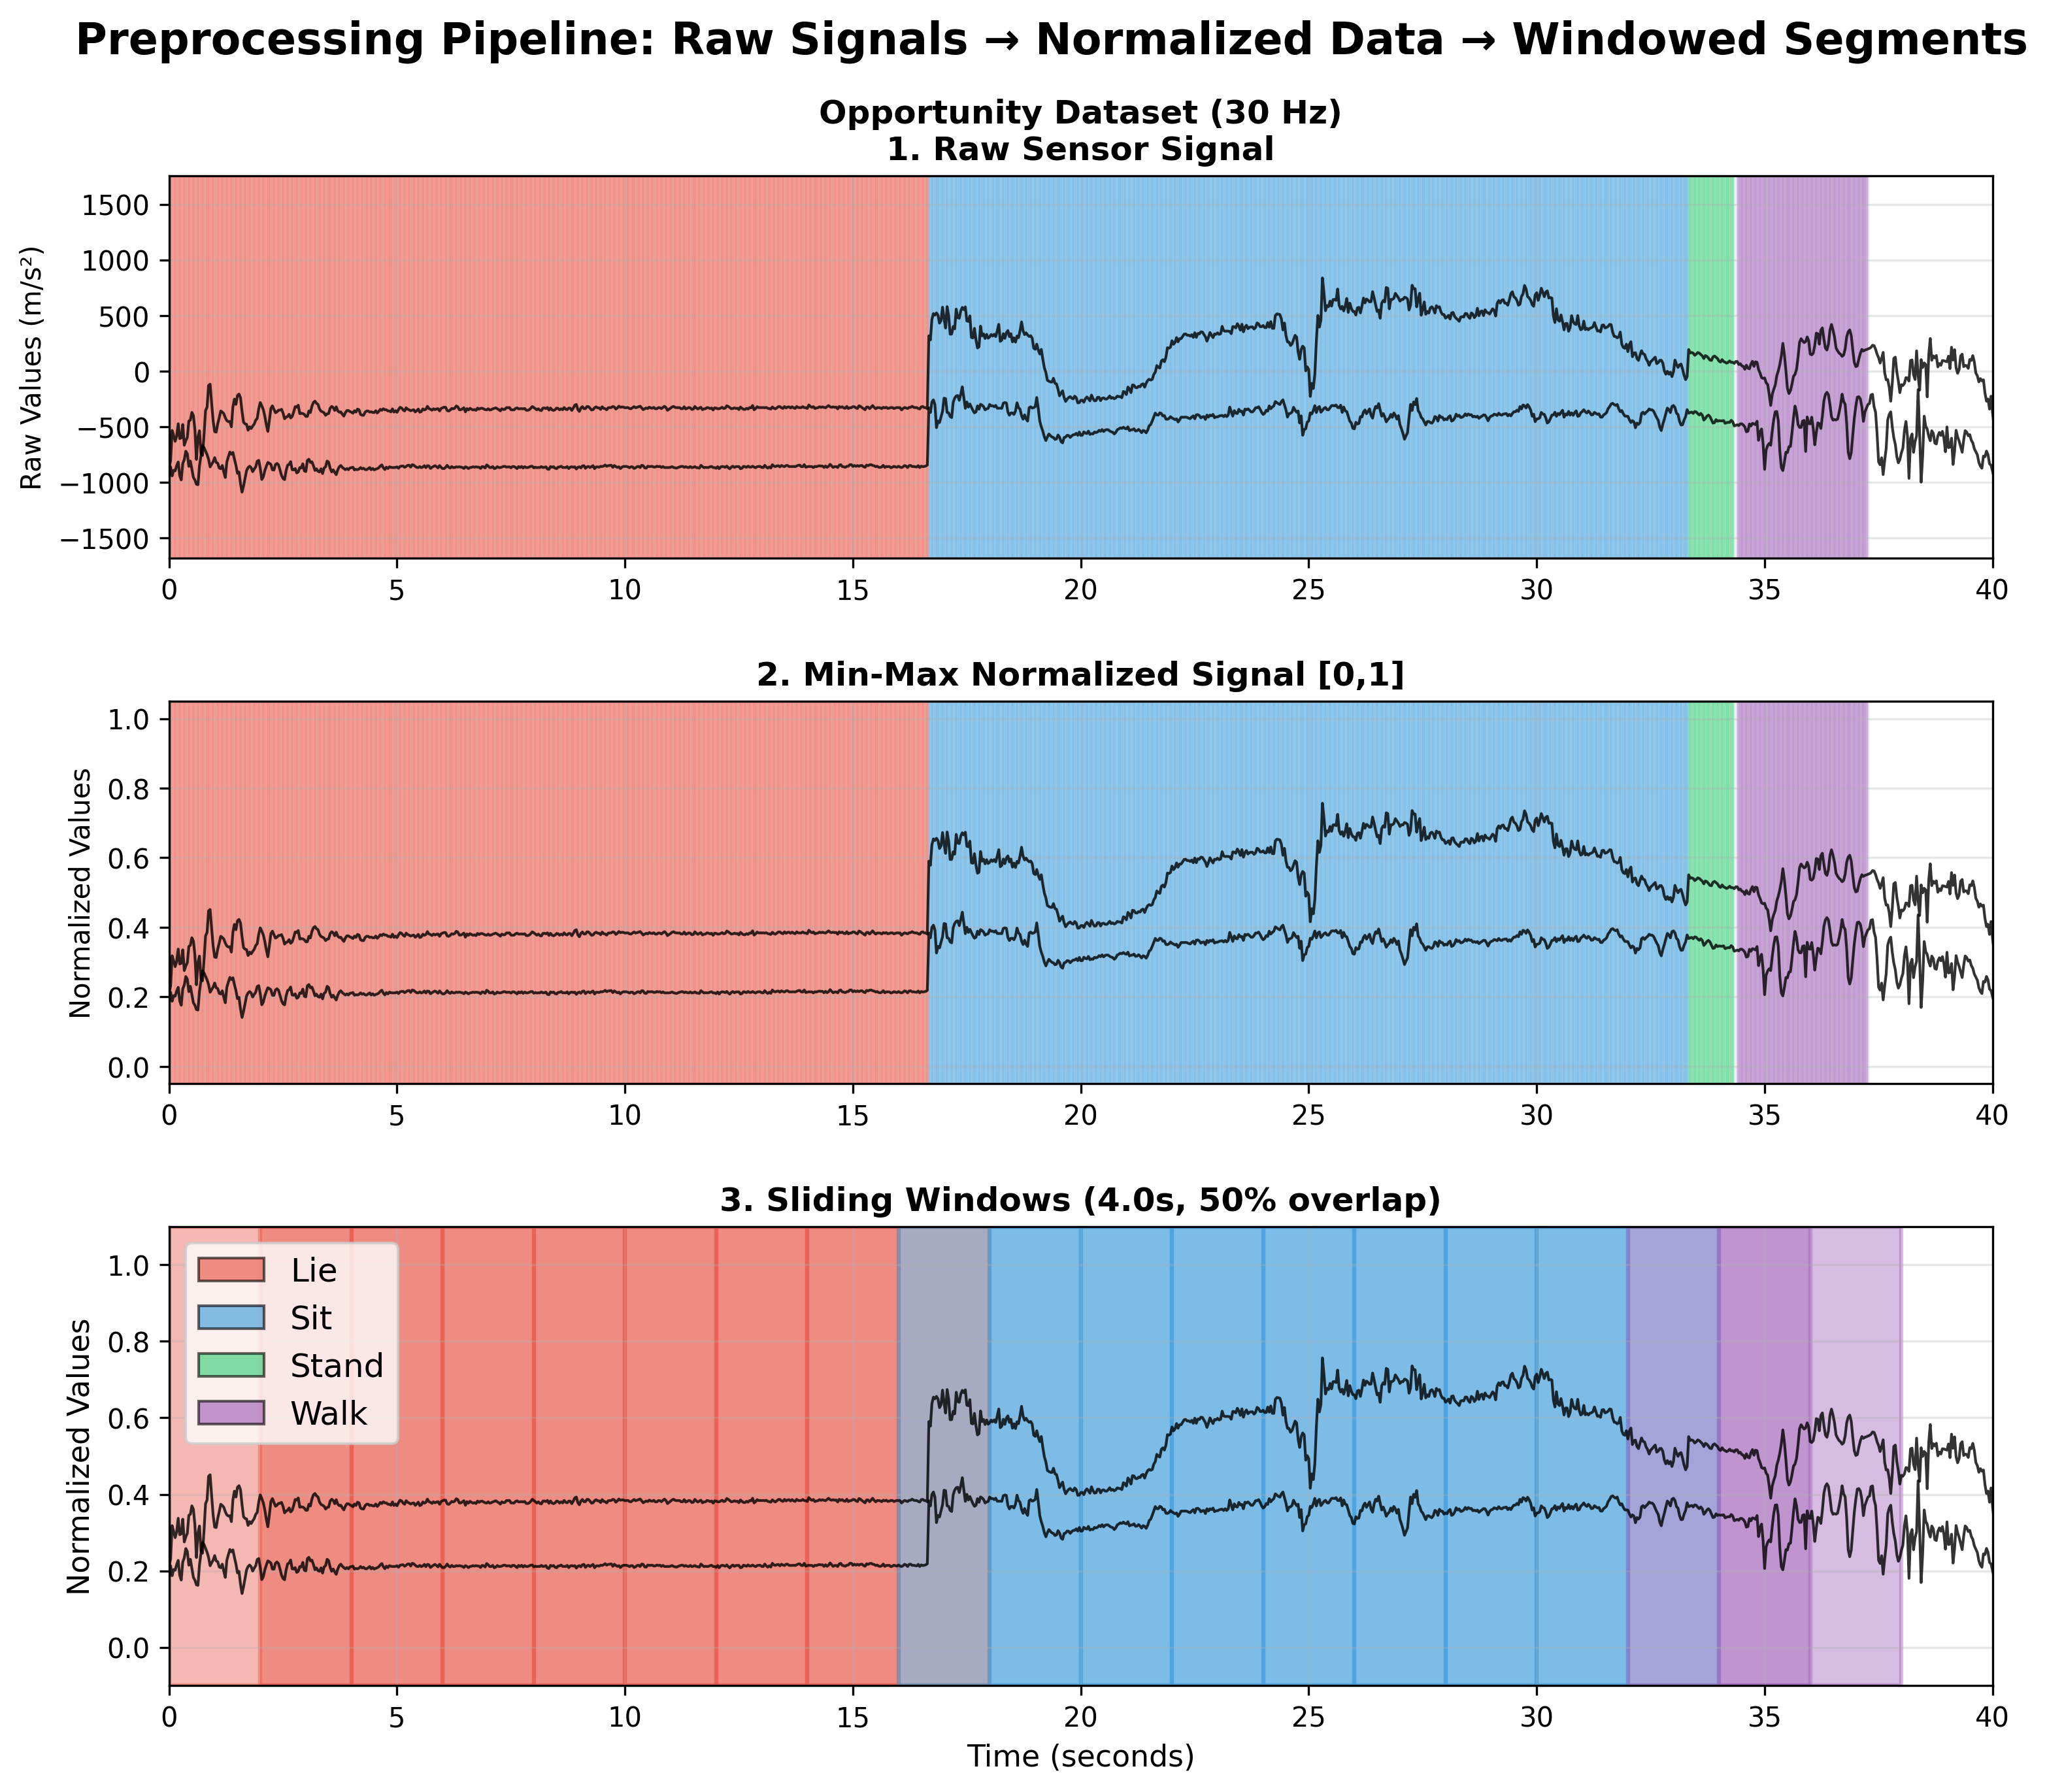
\includegraphics[width=0.9\textwidth]{images/chapter4_preprocessing_pipeline_opportunity.png}
    \caption{Διαδικασία προεπεξεργασίας χρονοσειρών αισθητήρων. Απεικονίζεται η πλήρης αλυσίδα από τα ακατέργαστα σήματα του συνόλου \en{OPPORTUNITY} μέσω κανονικοποίησης \en{min-max} στην επικαλυπτόμενη παραθυροποίηση με απόδοση ετικετών βάσει πλειοψηφικού κανόνα.}
    \label{fig:preprocessing_pipeline}
\end{figure}

\section{Παραγωγή Ασαφών Συναρτήσεων Συμμετοχής}

Η μετάβαση από τα κανονικοποιημένα παράθυρα στις ασαφείς αναπαραστάσεις αποτελεί το κεντρικό βήμα της μεθοδολογίας.
Η παρούσα εργασία συγκρίνει τρεις προσεγγίσεις:

\subsection{\en{Kernel Density Estimation (KDE)}}
Η \en{state of the art} μέθοδος \en{KDE} εκτιμά τη συνάρτηση πυκνότητας $f(x)$ ως:
\[
f(x) = \frac{1}{nh} \sum_{i=1}^{n} K\left(\frac{x - x_i}{h}\right)
\]
όπου $K$ είναι ο πυρήνας (συνήθως \en{Gaussian}), $h$ το εύρος ζώνης (\en{bandwidth}), και $n$ το πλήθος των σημείων. Παρά την υψηλή ακρίβεια, η \en{KDE} απαιτεί σημαντικούς πόρους μνήμης για την αποθήκευση όλων των δεδομένων εκπαίδευσης.

\subsection{\en{Normal Distribution Generator (NDG)}}
Ο αλγόριθμος \en{NDG} εκτιμά τη συνάρτηση πυκνότητας χρησιμοποιώντας άθροισμα πυρήνων. Η γενική μορφή είναι:

\[
\mu(x) = \frac{1}{n} \sum_{i=1}^{n} K(x, x_i, \sigma)
\]

όπου $x_i$ τα σημεία δεδομένων, $n$ το πλήθος των δειγμάτων, $\sigma$ η παράμετρος εύρους ζώνης και $K$ ο πυρήνας.

Η υλοποίηση υποστηρίζει διάφορους τύπους πυρήνων:
\begin{itemize}
    \item \textbf{\en{Gaussian}:} Ο πιο συνηθισμένος πυρήνας με ομαλή μείωση
    \item \textbf{\en{Epanechnikov}:} Βέλτιστος πυρήνας ως προς το μέσο τετραγωνικό σφάλμα
    \item \textbf{\en{Triangular}:} Γραμμική μείωση της επιρροής με την απόσταση
    \item \textbf{\en{Uniform}:} Ορθογωνικός πυρήνας με σταθερή τιμή εντός παραθύρου
    \item \textbf{\en{Quartic}:} Πυρήνας με πιο ομαλή μείωση από τον \en{Epanechnikov}
\end{itemize}

Μετά από πειράματα τα οποία θα αναλυθούν εκτενώς στο επόμενο κεφάλαιο, επιλέχθηκε να χρησιμοποιηθεί ο \en{Gaussian} πυρήνας με $\sigma = 0.1$. Οι επιλογές αυτές παρέχουν την καλύτερη ισορροπία μεταξύ ακρίβειας και υπολογιστικής αποδοτικότητας για τα δεδομένα αισθητήρων.

\subsection{\en{Streaming NDG (NDG-S)}}
Ο αλγόριθμος \en{NDG-S} προσαρμόζει τον \en{NDG} για επεξεργασία μεγάλων δεδομένων μέσω τμηματικής (\en{chunked}) επεξεργασίας:

\begin{enumerate}
    \item \textbf{Τμηματοποίηση δεδομένων:} Τα δεδομένα διαιρούνται σε τμήματα (\en{chunks}), με μέγεθος προσαρμόσιμο ανάλογα με τη διαθέσιμη μνήμη.
    
    \item \textbf{Επεξεργασία ανά τμήμα:} Για κάθε τμήμα $C_k$ υπολογίζεται μερική συνάρτηση συμμετοχής:
    \[
    \mu_k(x) = \frac{1}{|C_k| \sigma \sqrt{2\pi}} \sum_{x_i \in C_k} \exp\left(-\frac{(x - x_i)^2}{2\sigma^2}\right)
    \]
    
    \item \textbf{Συνδυασμός αποτελεσμάτων:} Η τελική συνάρτηση συμμετοχής προκύπτει από το μέσο όρο των μερικών συναρτήσεων:
    \[
    \mu(x) = \frac{1}{K} \sum_{k=1}^{K} \mu_k(x)
    \]
    όπου $K$ ο αριθμός των τμημάτων.
\end{enumerate}

Η διαφορά με τον κλασικό \en{NDG} είναι ότι ο \en{NDG-S} μπορεί να επεξεργαστεί δεδομένα που δεν χωρούν στη μνήμη, με το κόστος ελαφρώς μειωμένης ακρίβειας λόγω της τμηματικής επεξεργασίας.

\subsection{Προσέγγιση Ανά Αισθητήρα}

Στη μετάβαση από τον χρονικό χώρο των δεδομένων αισθητήρων στον χώρο των ασαφών συναρτήσεων συμμετοχής, υπήρχαν πολλές επιλογές για το πώς να συνδυάσουμε τα δεδομένα των διαφορετικών αισθητήρων.
Η επιλογή του υπολογισμού μιας συνάρτησης συμμετοχής ανά αισθητήρα έγινε συνειδητά για να εξυπηρετήσει τον διπλό στόχο της έρευνας: όχι μόνο την αναγνώριση δραστηριοτήτων αλλά και την αναγνώριση του τύπου και της θέσης των αισθητήρων.

Η προσέγγιση αυτή παράγει μία ξεχωριστή συνάρτηση συμμετοχής για κάθε αισθητήρα, διατηρώντας έτσι τα μοναδικά χαρακτηριστικά και την πληροφορία που φέρει ο καθένας. Αυτό επιτρέπει την ταυτόχρονη ανάλυση τόσο του περιεχομένου (τι δραστηριότητα εκτελείται) όσο και της πηγής (ποιος αισθητήρας την κατέγραψε).

\begin{figure}[ht]
    \centering
    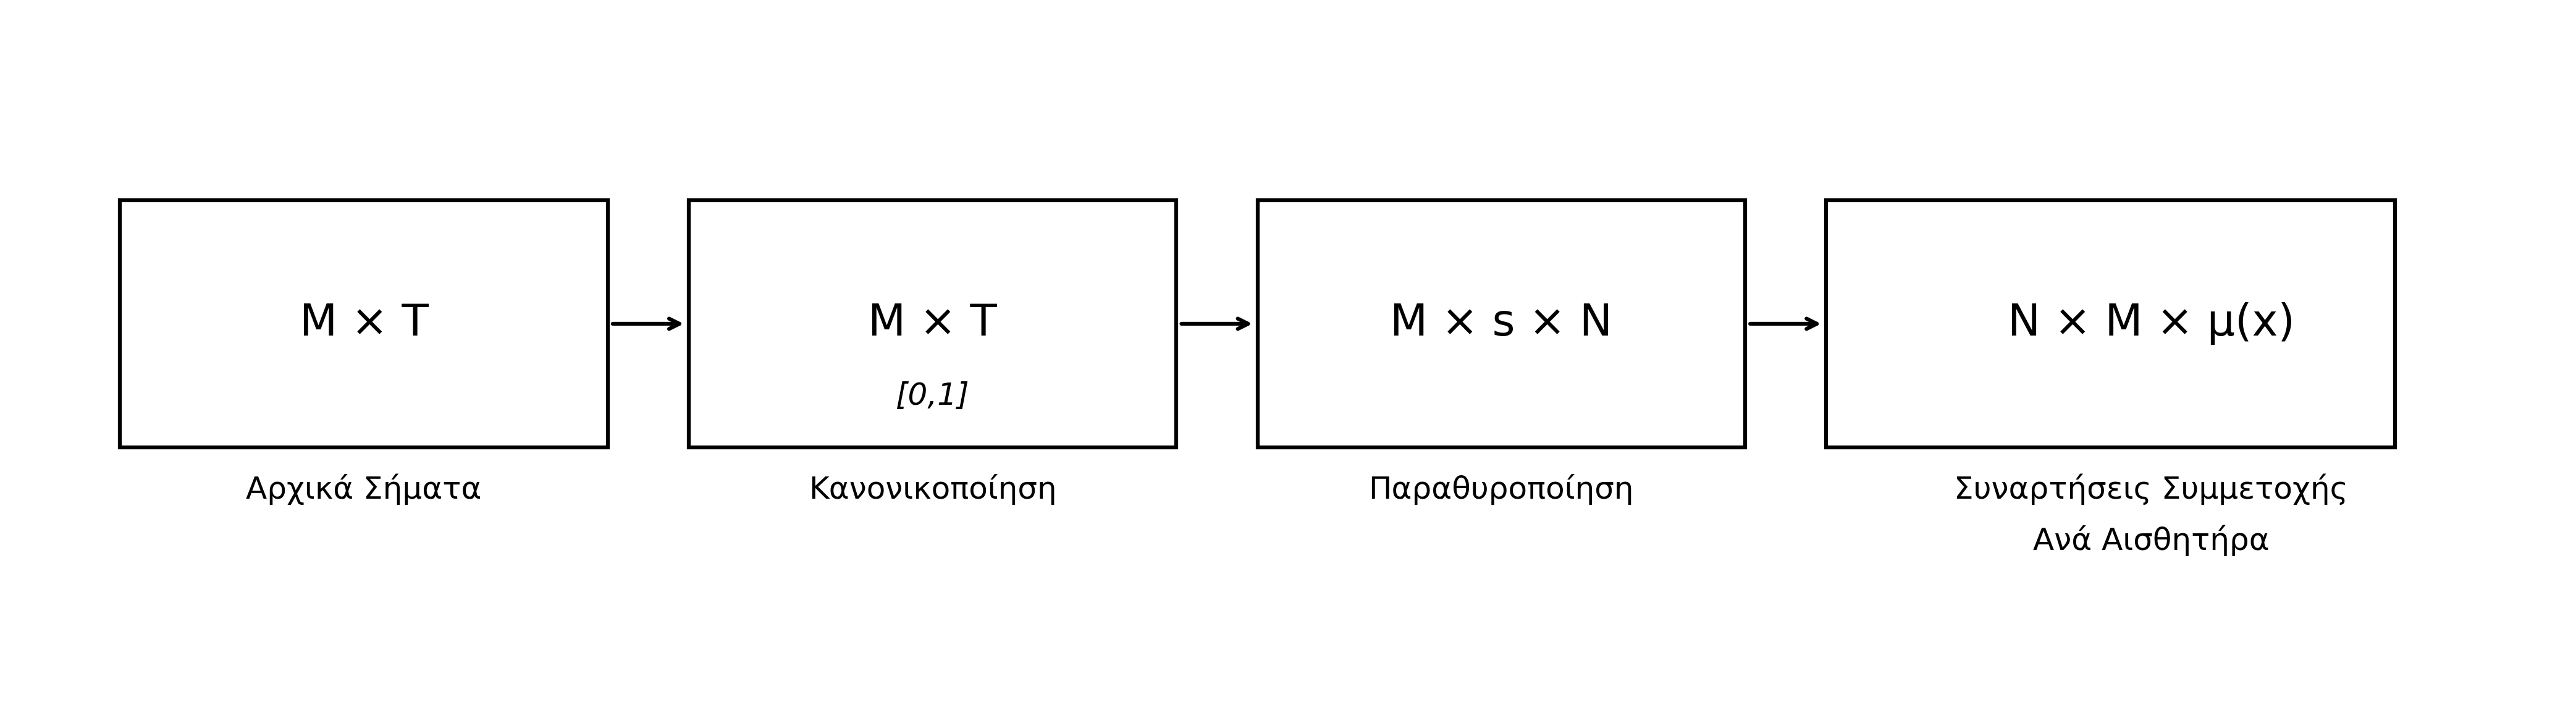
\includegraphics[width=0.9\textwidth]{images/minimal_per_sensor_flow.png}
    \caption{Διαστάσεις δεδομένων στην προσέγγιση ανά αισθητήρα, από τα αρχικά σήματα (\en{M×T}) έως τις τελικές \en{membership functions} (\en{N×M×μ(x)}). Όπου \en{M}: αριθμός αισθητήρων, \en{T}: χρονικά δείγματα, \en{s}: μέγεθος παραθύρου, \en{N}: αριθμός παραθύρων, \en{μ(x)}: \en{membership function values}}
    \label{fig:per_sensor_flow}
\end{figure}

\section{Πλαίσιο Μετρικών Ομοιότητας}

Η σύγκριση των ασαφών συναρτήσεων συμμετοχής απαιτεί εξειδικευμένες μετρικές που λαμβάνουν υπόψη τη συνεχή φύση των τιμών συμμετοχής στο διάστημα $[0,1]$. Η παρούσα εργασία υλοποιεί και αξιολογεί 16 μετρικές ομοιότητας που κατηγοριοποιούνται σε πέντε βασικές οικογένειες.

\subsection{Συνολοθεωρητικές Μετρικές}
Βασισμένες στη θεωρία ασαφών συνόλων, οι μετρικές αυτές εκμεταλλεύονται τις έννοιες της τομής και της ένωσης:

\begin{itemize}
    \item \textbf{\en{Jaccard Similarity}}: $J(\mu_1, \mu_2) = \frac{\int \min(\mu_1(x), \mu_2(x)) dx}{\int \max(\mu_1(x), \mu_2(x)) dx}$
    \item \textbf{\en{Dice Coefficient}}: $D(\mu_1, \mu_2) = \frac{2 \int \min(\mu_1(x), \mu_2(x)) dx}{\int \mu_1(x) dx + \int \mu_2(x) dx}$
    \item \textbf{\en{Overlap Coefficient}}: $O(\mu_1, \mu_2) = \frac{\int \min(\mu_1(x), \mu_2(x)) dx}{\min(\int \mu_1(x) dx, \int \mu_2(x) dx)}$
\end{itemize}

\subsection{Μετρικές Βασισμένες σε Απόσταση}
Μετατρέπουν μετρικές απόστασης σε μέτρα ομοιότητας:

\begin{itemize}
    \item \textbf{\en{Euclidean Similarity}}: $s_E = \frac{1}{1 + \sqrt{\sum_i (\mu_1(x_i) - \mu_2(x_i))^2}}$
    \item \textbf{\en{Hamming Similarity}}: Βασισμένη σε $s_H = \frac{1}{1 + \sum_i |\mu_1(x_i) - \mu_2(x_i)|}$
    \item \textbf{\en{Chebyshev Similarity}}: $s_C = 1 - \max_i |\mu_1(x_i) - \mu_2(x_i)|$ (για $[0,1]$ τιμές)
\end{itemize}

\subsection{Μετρικές Συσχέτισης}
Μετρούν γραμμικές και μη-γραμμικές σχέσεις μεταξύ των συναρτήσεων συμμετοχής:

\begin{itemize}
    \item \textbf{\en{Cosine Similarity}}: $\cos(\mu_1, \mu_2) = \frac{\sum_i \mu_1(x_i) \mu_2(x_i)}{\sqrt{\sum_i \mu_1^2(x_i)} \sqrt{\sum_i \mu_2^2(x_i)}}$
    \item \textbf{\en{Pearson Correlation}}: $r = \frac{\sum_i (\mu_1(x_i) - \bar{\mu_1})(\mu_2(x_i) - \bar{\mu_2})}{\sqrt{\sum_i (\mu_1(x_i) - \bar{\mu_1})^2} \sqrt{\sum_i (\mu_2(x_i) - \bar{\mu_2})^2}}$
    \item \textbf{\en{Cross-Correlation}}: Μέγιστη συσχέτιση με χρονικές μετατοπίσεις
\end{itemize}

\subsection{Πληροφοριοθεωρητικές Μετρικές}
Βασισμένες σε έννοιες από τη θεωρία πληροφοριών και την εντροπία:

\begin{itemize}
    \item \textbf{\en{Jensen-Shannon Similarity}}: $s_{JS} = 1 - \sqrt{JS(P||Q)}$, όπου $JS = \frac{1}{2}KL(P||M) + \frac{1}{2}KL(Q||M)$
    \item \textbf{\en{Bhattacharyya Coefficient}}: $BC = \sum_i \sqrt{p_i q_i}$
    \item \textbf{\en{Hellinger Similarity}}: $s_H = 1 - \frac{1}{\sqrt{2}}\sqrt{\sum_i (\sqrt{p_i} - \sqrt{q_i})^2}$
    \item \textbf{\en{Mutual Information}}: Βασισμένη σε εκτίμηση \en{histogram}
\end{itemize}

\subsection{Προχωρημένες Μετρικές}
Εξειδικευμένες μετρικές για συγκεκριμένες εφαρμογές:

\begin{itemize}
    \item \textbf{\en{Earth Mover's Distance Similarity}}: $s_{EMD} = \frac{1}{1 + EMD(\mu_1, \mu_2)}$ (βέλτιστη μεταφορά)
    \item \textbf{\en{Energy Distance Similarity}}: $s_E = \frac{1}{1 + |E_{12} - E_{11} - E_{22}|}$ 
    \item \textbf{\en{Harmonic Mean Similarity}}: $s_{HM} = \frac{1}{n}\sum_i \frac{2\mu_1(x_i)\mu_2(x_i)}{\mu_1(x_i) + \mu_2(x_i)}$
\end{itemize}

\subsection{Υπολογιστική Υλοποίηση}
Όλες οι μετρικές υλοποιούνται με διανυσματικές λειτουργίες \en{NumPy} για βέλτιστη απόδοση. Η αριθμητική ολοκλήρωση πραγματοποιείται με τον κανόνα του τραπεζίου, ενώ εφαρμόζεται κανονικοποίηση στο $[0,1]$ όπου απαιτείται.


\section{Πειραματικός Σχεδιασμός}
Η αξιολόγηση ακολουθεί προσέγγιση βασισμένη σε ανάκτηση όπου παράθυρα ερωτημάτων συγκρίνονται με βιβλιοθήκη επισημασμένων παραθύρων χρησιμοποιώντας μετρικές \en{Hit@k} και \en{Mean Reciprocal Rank (MRR)}.

\section{Πρωτόκολλο Αξιολόγησης RQ1}
Οι αλγόριθμοι \en{NDG-S} και \en{KDE} συγκρίνονται σε συνθετικά, \en{Opportunity}, και \en{PAMAP2} σύνολα δεδομένων μετρώντας υπολογιστικό χρόνο, χρήση μνήμης, και ακρίβεια προσέγγισης χρησιμοποιώντας \en{KL-divergence}.

\section{Πρωτόκολλο Αξιολόγησης RQ2}
Όλες οι μετρικές ομοιότητας αξιολογούνται σε εργασίες αναγνώρισης δραστηριοτήτων χρησιμοποιώντας ισορροπημένα σύνολα δεδομένων με στρωματοποιημένη δειγματοληψία, μετρώντας ακρίβεια ανάκτησης για διαφορετικούς τύπους ετικετών (\en{Locomotion}, \en{ML\_Both\_Arms}, \en{HL\_Activity}).

\section{Πρωτόκολλο Αξιολόγησης RQ3}
Η ευστάθεια μεταξύ συνόλων δεδομένων εκτιμάται υπολογίζοντας συσχετίσεις \en{Spearman rank} μεταξύ κατατάξεων απόδοσης μετρικών στα σύνολα δεδομένων \en{Opportunity} και \en{PAMAP2}.

\section{Πλαίσιο Στατιστικής Ανάλυσης}
Η στατιστική σημαντικότητα καθορίζεται χρησιμοποιώντας τεστ \en{Wilcoxon signed-rank} για ζευγαρωτές συγκρίσεις και τεστ \en{Friedman} για συγκρίσεις πολλαπλών μετρικών, με ανάλυση \en{Nemenyi post-hoc} για διαφορές ομάδων.

\section{Βελτιστοποίηση Απόδοσης}
Η ενοποιημένη προσέγγιση παραθύρων προυπολογίζει συναρτήσεις συμμετοχής μία φορά και τις επαναχρησιμοποιεί σε πολλαπλούς τύπους ετικετών, επιτυγχάνοντας σημαντική υπολογιστική επιτάχυνση για πειράματα πολλαπλών ετικετών.

\section{Στρατηγική Επικύρωσης}
Η διασταυρούμενη επικύρωση εκτελείται χρησιμοποιώντας στρωματοποιημένες διαιρέσεις για εξασφάλιση ισορροπημένης αναπαράστασης δραστηριοτήτων και τύπων αισθητήρων, με ξεχωριστές κατανομές εκπαίδευσης/ελέγχου για αποφυγή διαρροής δεδομένων.

\section{Λεπτομέρειες Υλοποίησης}
Όλοι οι αλγόριθμοι υλοποιούνται σε \en{Python} χρησιμοποιώντας \en{NumPy} για διανυσματικές λειτουργίες, με μηχανισμούς προσωρινής αποθήκευσης για συναρτήσεις συμμετοχής και παράλληλη επεξεργασία για υπολογισμούς ομοιότητας.

\section{Μετρικές Αξιολόγησης}
Οι κύριες μετρικές περιλαμβάνουν \en{Hit@1}, \en{Hit@5}, \en{MRR} για εργασίες ανάκτησης, συν μέτρα υπολογιστικής αποδοτικότητας (χρόνος εκτέλεσης, χρήση μνήμης) και δείκτες στατιστικής σημαντικότητας (τιμές \en{p}, μεγέθη επίδρασης).


\section{Σύνοψη κεφαλαίου}
% TODO: Ανακεφαλαίωση και σύνδεση με επόμενο κεφάλαιο.

%\chapter{Αποτελέσματα}

Σε αυτό το κεφάλαιο, θα παρουσιασθούν και θα αναλυθούν τα αποτελέσματα των πειραμάτων, όπως πρόκυψαν από τα βασικά ερευνητικά ερωτήματα και παρουσιάστηκαν στο Κεφάλαιο 5.

\section{Ερευνητικό Ερώτημα 1}

# Να μπει σε italic και ελληνικά:
# #### **RQ1: Can we make membership function computation efficient enough for real-time use?**
# **The Question:** Traditional KDE is too slow for IoT applications. Can our NDG-S algorithm achieve significant speedup while maintaining accuracy?

\subsection{Αναγνώριση βέλτιστων παραμέτρων για την πειραματική μέθοδο \en{NDG-S}}

\subsection{Συγκρίση αποδοτικότητας πειραματικής μεθόδου \en{NDG-S} με την \en{state-of-art} μέθοδο \en{KDE}}

\section{Ερευνητικό Ερώτημα 2}

# Να μπει σε italic και ελληνικά:
# ### **RQ2: Can per-sensor fuzzy membership functions improve activity recognition?**
# **The Question:** Traditional approaches treat all sensors equally. Can preserving individual sensor characteristics improve performance?

/subsection{Πειράμα αναγνωρίσης δραστηριότητας στο \en{Opportunity dataset} }

/subsection{Πειράμα πειραμάτος αναγνωρίσης δραστηριότητας στο \en{PAMAP2 dataset} }

\section{Ερευνητικό ερώτημσ 3}

#### **RQ3: Do our similarity metrics work consistently across different datasets?**
**The Question:** Will metrics that work well on one dataset also work on datasets with different sensors and sampling rates?

/subsection{Πειράμα αναγνωρίσης δραστηριότητας μεταξύ των \en{Opportunity} και \en{PAMAP2 datasets} }
%\chapter{Συμπεράσματα και μελλοντικές κατευθύνσεις}
%\include{chapter8}
Hello
\end